\documentclass{article}
\usepackage{geometry,amsmath,amssymb,graphicx,bbm,theorem,xr}
\usepackage[american]{babel}
\geometry{letterpaper}

%%%%%%%%%% Start TeXmacs macros
\newcommand{\Nu}{\mathrm{N}}
\newcommand{\assign}{:=}
\newcommand{\comma}{{,}}
\newcommand{\longhookrightarrow}{{\lhook\joinrel\relbar\joinrel\rightarrow}}
\newcommand{\nequiv}{\not\equiv}
\newcommand{\nin}{\not\in}
\newcommand{\nni}{\not\ni}
\newcommand{\nobracket}{}
\newcommand{\nocomma}{}
\newcommand{\nosymbol}{}
\newcommand{\tmmathbf}[1]{\ensuremath{\boldsymbol{#1}}}
\newcommand{\tmop}[1]{\ensuremath{\operatorname{#1}}}
\newcommand{\tmtextbf}[1]{{\bfseries{#1}}}
\newcommand{\tmtextit}[1]{{\itshape{#1}}}
\newcommand{\tmtextrm}[1]{{\rmfamily{#1}}}
\newcommand{\tmtextup}[1]{{\upshape{#1}}}
\newcommand{\um}{-}
\newcommand{\upl}{+}
\newenvironment{itemizedot}{\begin{itemize} \renewcommand{\labelitemi}{$\bullet$}\renewcommand{\labelitemii}{$\bullet$}\renewcommand{\labelitemiii}{$\bullet$}\renewcommand{\labelitemiv}{$\bullet$}}{\end{itemize}}
\newenvironment{proof}{\noindent\textbf{Proof\ }}{\hspace*{\fill}$\Box$\medskip}
\newtheorem{definition}{Definition}
\numberwithin{definition}{section}
\newtheorem{lemma}{Lemma}
\numberwithin{lemma}{section}
\newtheorem{proposition}{Proposition}
\numberwithin{proposition}{section}
{\theorembodyfont{\rmfamily}\newtheorem{remark}{Remark}
\numberwithin{remark}{section}
}
%%%%%%%%%% End TeXmacs macros

\newcommand{\D}{\mathcal{D}} \newcommand{\supp}{supp}
\newcommand{\proofexplanation}[1]{(#1)}
\newcommand{\C}{{\mathbbm{C}}}\newcommand{\Z}{{\mathbbm{Z}}}
\newcommand{\Sp}{{\mathbbm{S}}} \newcommand{\R}{{\mathbbm{R}}}
\newcommand{\mybra}[1]{(#1)} \newcommand{\mysbra}[1]{\left[#1\right]}
\newcommand{\mycbra}[1]{\left\{#1\right\}}
\externaldocument{master_master2}
\externaldocument{master_master3}

\begin{document}

\title{Study of symmetry breaking operators of indefinite orthogonal groups $O( p, q)$.\\ 
I. Geometry.}
\author{T. Kobayashi, O. Leontiev}
\maketitle

{\tableofcontents}

\section{Introduction}

\subsection{Motivation and Background}

Given $G$ a Lie group and $G'$ its closed subgroup, a large amount of research
in representation theory can very roughly be said to be associated with the
problem of relating representations of $G$ with representations of $G'$. It is
interesting that this problem is ``two-sided'': that is, one can be interested
in constructing representations of $G$ starting with that of $G'$, or one can
be interested in decomposing given representation of $G$ into representations
of $G'$.

Regarding the former, the standard way of obtaining representations of $G$
from that of $G'$ is a so-called induction. In particular, if one starts with
the trivial representation of $G'$, proceeding in this way he arrives at the
representation of $G$ on $L^2 ( G / G')$. Trying to understand the latter
space, one essentially finds himself in the realm of harmonic analysis,
deriving Plancherel formulas etc. Another important special case that
attracted considerable attention is the case when one start with the trivial
representation of $G'$ and inducts to $G' \times G'$ (we see $G'$ as a
subgroup of $G' \times G'$ via the diagonal embedding). It was worked upon by
Gelfand and his students {\cite{gelfand1966generalized}} in '50s ,
Harish-Chandra {\cite{harishchandra1978harmonic}} \ in '70s, T. Oshima
{\cite{oshima1984description}}, P. Delorme {\cite{delorme1998plancherel}}, T.
Kobayashi
{\cite{kobayashi1994discrete1}},{\cite{kobayashi1998discrete2}},{\cite{kobayashi1998discrete3}}
and many others in '80s-'90s.

On the other hand, the latter problem (decomposing given
infinitely-dimensional representation $\pi$ of $G$ into representations $\tau$
of noncompact $G'$) appears to be more formidable with systematic study
beginning no earlier than in '90s. The simplest setting is that of
representation $\pi$ of $G$ decomposing as a discrete sum of irreducible
representations $\tau$ of $G'$. One is then interested in computing
multiplicities (i.e. number of times given $\tau$ appears in a sum) and this
can be done via combinatorial techniques. In general, however, infinitely
dimensional representation of $G$ \tmtextit{cannot} be decomposed into the
direct sum of irreducible representations of $G'$ and one should restrict
himself to a particularly ``nice'' settings (see {\cite{kobayashi2015program}}
for a thorough discussion). What is more, one finds himself in a situation
when he has several definitions for ``multiplicity'' and these in general are
\tmtextit{not} equal. One particularly well-behaved is $m ( \pi, \tau) \assign
\dim \tmop{Hom}_{G'} ( \pi |_{G'}, \tau)$ the dimension of $G'$-intertwining
operators or, as one sometimes calls them, \tmtextit{symmetry breaking
operators}. Finally, it \tmtextit{does not} happen in general that $\dim
\tmop{Hom}_{G'} ( \pi |_{G'}, \tau)$ are all finite, so one should further
restrict himself (see {\cite{kobayashi2014classification}} for classification
of pairs $( G, G')$ when multiplicities \tmtextit{are} always finite).

One particularly nice setting is that of $( G, G') = ( O ( p + 1, q), O ( p,
q))$. On the one hand, this setting is well-behaved in the sense that one does
not face none of the anomalies mentioned in the previous paragraph. In
particular, for $O ( n + 1, 1) \supset O ( n, 1)$ the complete classification
and explicit construction of all symmetry breaking operators between
degenerate principal series was accomplished in {\cite{kobayashi2015symmetry}}
by T. Kobayashi and B. Speh recently.

On the other hand, this setting is important to number theory (cf.
Gross-Prasad conjecture {\cite{gan2011symplectic}}, Rankin-Cohen bracket
{\cite{kobayashi2015differential1}},{\cite{kobayashi2015differential2}}),
conformal geometry (cf. Juhl conformal differential operators
{\cite{juhl2009families}}) and, of course, representation theory. Already the
special cases are very important. In particular, the latter sections of
{\cite{kobayashi2015symmetry}} contain some of the applications for $O ( n +
1, 1) \supset O ( n, 1)$ case. Another particular case $O ( 2, 2) \supset O (
2, 1)$ (see {\cite{clerc2011generalized}}) is equivalent to the problem of
finding invariant trilinear forms on representations of $\tmop{SL}_2 (
\mathbbm{R})$.

Based on the (quite general) techniques introduced in
{\cite{kobayashi2015symmetry}}, we attempt to investigate the symmetry
breaking for $( G, G') = ( O ( p + 1, q), O ( p, q))$ case.

\subsection{Main results}

Letting $p, q \geqslant 1$ and $( G, G') : = ( O ( p + 1, q + 1), O ( p, q +
1))$, the purpose of this paper is to answer the following

{\noindent}\tmtextbf{Question. }\tmtextit{For given $( \lambda, \nu) \in
\mathbbm{C}^2$ explicitly describe the vector space of $\tmop{Hom}_{G'} ( I (
\lambda), J ( \nu))$ of $G'$-intertwining operators between degenerate
principal series $I ( \lambda)$ and $J ( \nu)$ of $G$ and $G'$ respectively.
In particular, find the explicit form of a basis.}{\hspace*{\fill}}{\medskip}

{\noindent}This task is made possible by the following result, which is
essentially {\cite[thm. 3.16]{kobayashi2015symmetry}}

{\noindent}\tmtextbf{Proposition. }\tmtextit{(prop. \ref{sol:prop-sol} below)
For every $( \lambda, \nu) \in \mathbbm{C}^2$ we have $\tmop{Hom}_{G'} ( I (
\lambda), J ( \nu)) \simeq \mathcal{S} \tmop{ol} ( \mathbbm{R}^{p, q} ;
\lambda, \nu)$, where $\mathcal{S} \tmop{ol} ( \mathbbm{R}^{p, q} ; \lambda,
\nu)$ denotes the space of generalized function $F \in \mathcal{D}' (
\mathbbm{R}^{p, q})$, that:
\begin{enumerate}
  \item are homogeneous of degree $\lambda - \nu - n$;
  
  \item even on $\mathbbm{R}^{p, q}$;
  
  \item satisfy $F ( m \cdot) = F ( \cdot)$ for every $m \in O ( p, q)_{e_p}
  \assign \{ m \in O ( p, q) | m \cdot e_p = e_p \}$;
  
  \item for every $b, x_0 \in \mathbbm{R}^{p, q}$ such that $b_p = 0$ and $c_b
  ( x_0) : = 1 - 2 Q ( b, x_0) + Q ( x_0) Q ( b) \neq 0$ we have
  \begin{eqnarray}
    & | c_b ( \cdot) |^{\lambda - n} F ( \psi_b ( \cdot)) = F (\cdot)
    \hspace{1em} \tmop{near} \hspace{1em} x_0, &  \nonumber\\
    & \psi_b ( x) \assign \frac{x - Q (x) b}{c_b ( x)} . &  \nonumber
  \end{eqnarray}
\end{enumerate}}{\hspace*{\fill}}{\medskip}

{\noindent}Now, the main results of the paper are as follows:

{\noindent}\tmtextbf{Proposition. }\tmtextit{(see sec. \ref{sec:doublePGP})
Let $Q$ be $( p, q)$-quadratic form and $P, P'$ denote the maximal parabolic
subgroups of $G, G'$ respectively. Then,
\begin{enumerate}
  \item one can explicitly list the $P' \backslash G / P$ coset (see prop.
  \ref{doublePGP:prop-orbitdeco});
  
  \item pullback of $P' \backslash G / P$ cosets under the $\mathbbm{R}^{p, q}
  \simeq N_- \hookrightarrow G / P$ embedding are as follows:
  \[ \left\{ \begin{array}{ll}
       \{ x_p \neq 0, Q \neq 0 \} \sqcup \{ x_p \neq 0, Q = 0 \} \sqcup \{ x_p
       = 0, Q \neq 0 \} \sqcup \{ 0 \}, & p = 1\\
       \{ x_p \neq 0, Q \neq 0 \} \sqcup \{ x_p \neq 0, Q = 0 \} \sqcup \{ x_p
       = 0, Q \neq 0 \} \sqcup \{ x_p = 0, Q = 0 \} \backslash \{ 0 \} \sqcup
       \{ 0 \}, & p > 1
     \end{array} \right. \]
  where, say $\{ x_p \neq 0, Q \neq 0 \} \assign \{ x \in \mathbbm{R}^{p, q} |
  Q ( x) \neq 0, x_p \neq 0 \}$;
  
  \item $P' N_- P = G$.
\end{enumerate}}{\hspace*{\fill}}{\medskip}

{\noindent}\tmtextbf{Remark. }In particular, the third item supplies necessary
hypothesis for the proof of $\tmop{Hom}_{G'} ( I ( \lambda), J ( \nu)) \simeq
\mathcal{S} \tmop{ol} ( \mathbbm{R}^{p, q} ; \lambda, \nu)$ isomorphism, while
the second item implies that an element of $\mathcal{S} \tmop{ol} (
\mathbbm{R}^{p, q} ; \lambda, \nu)$ can have its support equal only to: $\{ 0
\}$, $P \assign \{ x \in \mathbbm{R}^{p, q} | x_p = 0 \}$, $C \assign \{ x \in
\mathbbm{R}^{p, q} | Q ( x) = 0 \}$, $P \cap C$, $C \cup P$ or
$\mathbbm{R}^{p, q}$.

We will therefore use the notation $\mathcal{S} \tmop{ol}_S ( \mathbbm{R}^{p,
q} ; \lambda, \nu)$ to denote elements of $\mathcal{S} \tmop{ol} (
\mathbbm{R}^{p, q} ; \lambda, \nu)$ which are supported inside some fixed
$S$.{\hspace*{\fill}}{\medskip}

{\noindent}\tmtextbf{Proposition. }\tmtextit{We have the following:
\begin{enumerate}
  \item (prop. \ref{supp-R:prop-3}) for $\lambda, \nu \in \mathbbm{C}$ with
  $\lambda - \nu \nin -\mathbbm{Z}_{\geqslant 0}$ one can extend the
  well-defined product of generalized functions
  \[ \frac{| x_p |^{\lambda + \nu - n}}{\Gamma ( ( \lambda + \nu - n + 1) /
     2)} \cdot \frac{| Q |^{- \nu}}{\Gamma ( ( 1 - \nu) / 2)} \in \mathcal{D}'
     ( \mathbbm{R}^{p, q} \backslash \{ 0 \}) \]
  to an element $K_{\lambda, \nu}^{\mathbbm{R}^n}$ of $\mathcal{S} \tmop{ol} (
  \mathbbm{R}^{p, q} ; \lambda, \nu)$. One can also explicitly determine its
  support (see prop. \ref{KR-normalization-recur:prop-supp}), which is
  generically equal to $\mathbbm{R}^{p, q}$;
  
  \item (prop. \ref{supp-Q:prop-sol-extending}) For $\nu \nin
  2\mathbbm{Z}_{\geqslant 0} + 1$ $\mathcal{S} \tmop{ol}_{\{ 0 \}} (
  \mathbbm{R}^{p, q} ; \lambda, \nu) =\mathcal{S} \tmop{ol}_C (
  \mathbbm{R}^{p, q} ; \lambda, \nu)$, while for $\nu \in
  2\mathbbm{Z}_{\geqslant 0} + 1$ fixed and $\lambda \in \{ \lambda \in
  \mathbbm{C} | \lambda - \nu \in -\mathbbm{Z}_{\geqslant 0} \}$ one can
  extend the well-defined product of generalized functions
  \[ \left\{ \begin{array}{ll}
       \delta^{( \nu - 1)} ( Q) \cdot | x_p |^{\lambda + \nu - n}, & p = 1\\
       \delta^{( \nu - 1)} ( Q) \cdot \frac{| x_p |^{\lambda + \nu -
       n}}{\Gamma ( ( \lambda + \nu - n + 1) / 2)}, & p > 1
     \end{array} \right. \]
  to an element $K_{\lambda, \nu}^C$ of $\mathcal{S} \tmop{ol}_C (
  \mathbbm{R}^{p, q} ; \lambda, \nu) \backslash\mathcal{S} \tmop{ol}_{\{ 0 \}}
  ( \mathbbm{R}^{p, q} ; \lambda, \nu)$. One can also explicitly determine its
  support (see prop. \ref{supp-Q:prop-supp-xnoq0}), which is generically equal
  to $C$;
  
  \item (sec. \ref{sec:supp-P}) For $\lambda + \nu - n = - 1 - 2 k, \; k \in
  \mathbbm{Z}_{\geqslant 0}$ the distribution
  \begin{eqnarray}
    & K^P_{\lambda, \nu} \assign \sum_{i = 0}^k \frac{(- 1)^i (2 k) !
    (\nu)^{}_i}{(2 k - 2 i) !i!} \delta^{(2 k - 2 i)} (x_p) \otimes
    \tilde{Q}_i \in \mathcal{D}' ( \mathbbm{R}^{p, q} ; \lambda, \nu), & 
    \nonumber\\
    & (\nu)^{}_i \assign \nu (\nu + 1) \ldots (\nu + i - 1), &  \nonumber\\
    & \tilde{Q}_i \assign \left\{ \begin{array}{ll}
      \tilde{Q}_+^{- \nu - i} + \tilde{Q}_-^{- \nu - i}, & i \in 2 \Z_{\ge 0},
      p \geqslant 2\\
      \tilde{Q}_+^{- \nu - i} - \tilde{Q}_-^{- \nu - i}, & i \in 2 \Z_{\ge 0}
      + 1, p \geqslant 2\\
      | \tilde{Q} |^{- \nu - i}, & i \in 2 \Z_{\ge 0}, p = 1\\
      - | \tilde{Q} |^{- \nu - i}, & i \in 2 \Z_{\ge 0} + 1, p = 1
    \end{array} \right. &  \nonumber
  \end{eqnarray}
  (with $\tilde{Q}$ being $( p - 1, q)$-quadratic form) is an element of
  $\mathcal{S} \tmop{ol}_P ( \mathbbm{R}^{p, q} ; \lambda, \nu)$ well-defined
  for $\nu \in \mathbbm{C}$ outside some discrete subset. Again, support is
  generically equal to $P$ and can be explicitly determined (see sec.
  \ref{sec:KP-normalization}).
\end{enumerate}}{\hspace*{\fill}}{\medskip}

{\noindent}\tmtextbf{Remark. }Three families $K_{\lambda,
\nu}^{\mathbbm{R}^n}$, $K_{\lambda, \nu}^C$ and $K_{\lambda, \nu}^P$ are thus
constructed for parameters outside some codimension one subsets of
$\mathbbm{C}^2$, $\mathbbm{C}$ and $\mathbbm{C}$ respectively. It turns out
that they have poles at these subsets, hence in order to extend these families
to the whole $\mathbbm{C}^2$, $\mathbbm{C}$ and $\mathbbm{C}$ respectively,
one should ``normalize'' them, that is, divide by some meromorphic function in
order to eliminate poles. This situation is much similar to the way one
normalizes generalized function $x_+^{\lambda}$ to show that $x_+^{\lambda} /
\Gamma ( \lambda + 1)$ is holomorphic (see {\cite[sec.
1.3.5]{gelfand1980distribution}}).{\hspace*{\fill}}{\medskip}

{\noindent}\tmtextbf{Proposition. }\tmtextit{We have the following:
\begin{enumerate}
  \item (sec. \ref{sec:KC-normalization}) Depending on $p, q \in
  \mathbbm{Z}_{\geqslant 1}$ and $\nu \in 2\mathbbm{Z}_{\geqslant 0} + 1$, one
  can find meromorphic function $N$ so that $K_{\lambda, \nu}^C / N$
  holomorphically extends to all $\lambda \in \mathbbm{C}$ to give a nonzero
  element of $\mathcal{S} \tmop{ol}_C ( \mathbbm{R}^{p, q} ; \lambda, \nu)$.
  Its support is explicitly determined.
  
  \item (sec. \ref{sec:KP-normalization}) Depending on $p, q \in
  \mathbbm{Z}_{\geqslant 1}$ and $k \assign - ( \lambda + \nu - n + 1) / 2$,
  one can find meromorphic function $N$ so that $K_{\lambda, \nu}^P / N$
  holomorphically extends to all $\nu \in \mathbbm{C}$ ($\lambda$ is
  determined by $\nu$ subject to $\lambda + \nu - n = - 1 - 2 k$ condition) to
  give a nonzero element of $\mathcal{S} \tmop{ol}_P ( \mathbbm{R}^{p, q} ;
  \lambda, \nu)$. Its support is explicitly determined.
  
  \item (sec. \ref{sec:KR-normalization-even}) For $q \in 2\mathbbm{Z}$ and
  depending on $p, q \in \mathbbm{Z}_{\geqslant 1}$, one can find meromorphic
  function $N$ so that $K_{\lambda, \nu}^{\mathbbm{R}^n} / N$ holomorphically
  extends to all $ ( \lambda, \nu) \in \mathbbm{C}^2$ to give an element of
  $\mathcal{S} \tmop{ol}_{} ( \mathbbm{R}^{p, q} ; \lambda, \nu)$ which is
  nonzero outside the discrete subset of $\mathbbm{C}^2$.
\end{enumerate}}{\hspace*{\fill}}{\medskip}

\subsection{Organization of the paper}

Following the style of {\cite{kobayashi2015symmetry}} it was attempted to make
the exposition detailed, elementary and as self-contained as possible.
Regarding the latter, the effort was made to clearly state all the statements
that we use without proof as ``facts'' and give clear references. The notable
exception to this are the statements from {\cite{kobayashi2015symmetry}}: we
use these within our proofs, still, hopefully, with clear indication of which
statements and where were used.

Now, the remaining sections are organized as follows:
\begin{itemizedot}
  \item in sections \ref{sec:holomorphicity-preserving} to
  \ref{sec:pull-tensor-mult} miscellaneous results are collected. These will
  be used in latter sections, mostly in and after the section \ref{sec:lem67};
  they are independent of other sections and (largely) of each other; we
  suggest to omit them on the first reading and return to them later as
  necessary;
  
  \item in section \ref{sec:def-n-nots} objects that we are dealing with are
  defined (the most importantly, groups $G \supset G'$ and their degenerate
  principal series $I ( \lambda)$ and $J ( \nu)$ respectively), the main goal
  of the paper is also stated;
  
  \item in section \ref{sec:doublePGP} two crucial results are stated and
  proven. Of these the first one is that $P' N_- P = G$ equality holds. It
  provides necessary hypothesis to apply {\cite[thm
  3.16]{kobayashi2015symmetry}} which sets up the isomorphism \
  $\tmop{Hom}_{G'} ( I ( \lambda), J ( \nu)) \simeq \mathcal{S} \tmop{ol} (
  \mathbbm{R}^{p, q} ; \lambda, \nu)$. The second one is the description of
  $P' \backslash G / P$ double coset space and description of pullback of
  these cosets under the $N_- \hookrightarrow G / P$ embedding. It allows us
  to predict what supports elements of $\mathcal{S} \tmop{ol} (
  \mathbbm{R}^{p, q} ; \lambda, \nu)$ may have;
  
  \item in section \ref{sec:sol} $\mathcal{S} \tmop{ol} ( \mathbbm{R}^{p, q} ;
  \lambda, \nu)$ is formally defined and it is shown to be isomorphic with the
  space of SBOs $\tmop{Hom}_{G'} ( I ( \lambda), J ( \nu))$ for every fixed
  pair of parameters $( \lambda \comma \nu) \in \mathbbm{C}^2$;
  
  \item in section \ref{sec:n-nonequiv} a counter-example related to the
  notions introduced in section \ref{sec:sol} is constructed; it can be
  omitted without the loss of continuity;
  
  \item in \ref{sec:lem67} system of equations that define $\mathcal{S}
  \tmop{ol} ( \mathbbm{R}^{p, q} ; \lambda, \nu)$ is explicitly solved, but on
  a smaller set $\{ x \in \mathbbm{R}^{p, q} | Q ( x) \neq 0 \}$ (where $Q$ is
  a $( p, q)$-quadratic form);
  
  \item in sections \ref{sec:supp-R}, \ref{sec:supp-P} and \ref{sec:supp-Q}
  elements of $\mathcal{S} \tmop{ol} ( \mathbbm{R}^{p, q} ; \lambda, \nu)$ are
  constructed, that are supported within $\mathbbm{R}^{p, q}$, $\{ x \in
  \mathbbm{R}^{p, q} | x_p = 0 \}$ and $\{ x \in \mathbbm{R}^{p, q} | Q ( x) =
  0 \}$ respectively for $( \lambda, \nu)$ lying in some open subsets of
  $\mathbbm{C}^2$ (different for all three cases). These elements are
  constructed, so that they depend on $( \lambda, \nu)$ holomorphically;
  
  \item in section \ref{sec:diffSBO} for all $( \lambda, \nu) \in
  \mathbbm{C}^2$ elements of $\mathcal{S} \tmop{ol} ( \mathbbm{R}^{p, q} ;
  \lambda, \nu)$ that are supported within $\{ 0 \}$ are classified; these
  correspond to differential SBO under the correspondence $\tmop{Hom}_{G'} ( I
  ( \lambda), J ( \nu)) \simeq \mathcal{S} \tmop{ol} ( \mathbbm{R}^{p, q} ;
  \lambda, \nu)$;
  
  \item in section \ref{sec:k-finite} a method to analytically continuate
  families of elements of $\mathcal{S} \tmop{ol} ( \mathbbm{R}^{p, q} ;
  \lambda, \nu)$ to a larger parameter sets is introduced;
  
  \item in sections \ref{sec:KC-normalization}, \ref{sec:KP-normalization} and
  \ref{sec:KR-normalization-even} definitions of $K_{\lambda, \nu}^C$,
  $K_{\lambda, \nu}^P$ and $K_{\lambda, \nu}^{\mathbbm{R}^n}$ made in sections
  \ref{sec:supp-Q}, \ref{sec:supp-P} and \ref{sec:supp-R} respectively are
  extended to all parameters $( \lambda, \nu) \in \mathbbm{C}^2$, so that
  holomorphic dependence is preserved. For $K_{\lambda, \nu}^{\mathbbm{R}^n}$
  this is done under the assumption $q \in 2\mathbbm{Z}$;
  
  \item section \ref{sec:knappstein} is an application of techniques
  introduced in {\cite{kobayashi2015symmetry}} and used in this paper, to the
  problem of finding a concrete form of $G$-invariant $I ( \lambda)
  \rightarrow I ( n - \lambda)$ operator in a relatively elementary and
  straightforward way; the obtained results parallel some of that of
  {\cite{KO1}}.
\end{itemizedot}
Starting from section \ref{sec:doublePGP} all sections have the same
structure: first, every section opens with a brief introduction. Next, three
subsections follow. The first one, ``Main results'' contains the statements of
main propositions and definitions this section contains. Next, subsection
``Auxiliary lemmas'' follow, containing stated and immediately proven lemmas
that we use to prove the main results of the section. Finally, in the
subsection ``Proofs'' main results of the section are proven.

\subsection{Acknowledgments}

I'd like to thank my supervisor Toshiyuki Kobayashi who brought this topic to
my attention and taught me all the techniques necessary.

\section{Holomorphicity preserving}\label{sec:holomorphicity-preserving}

In this note we attempt to inspect a few operations on distributions defined
in {\cite{hormander1983analysis}} and investigate them in terms of preserving
holomorphicity.

\subsection{Facts}

We shall be interested in investigating the following statements shown in
{\cite{hormander1983analysis}}:

{\noindent}\tmtextbf{Fact \tmtextup{1}.
}\tmtextit{\label{holomorphicity-preserving:fact-homog}{\cite[thm.
3.2.3]{hormander1983analysis}} If $u \in \mathcal{D}' ( \mathbbm{R}^n - \{ 0
\})$ is homogeneous of degree $a \in \mathbbm{C}\backslash ( - n
-\mathbbm{Z}_{\geqslant 0})$, it's homogeneous extension $\dot{u} \in
\mathcal{D}' ( \mathbbm{R}^n)$ exists and is unique subject to homogeneity
requirement. Moreover, for arbitrary $\psi \in C_0^{\infty} ( \mathbbm{R}^n
\backslash \{ 0 \})$ satisfying $\forall x \neq 0, \; \int_0^{\infty} \psi ( t
x) d t / t = 1$ we have
\[ \langle \dot{u}, \varphi \rangle = \langle u, x \mapsto \psi ( x) \cdot
   \langle t_+^{a + n - 1}, t \mapsto \varphi ( t x) \rangle \rangle
\]}{\hspace*{\fill}}{\medskip}

\begin{definition}
  {\cite[sec. 8.2]{hormander1983analysis}} For $X \subset \mathbbm{R}^n$ open
  and $\Gamma \subset X \times ( \mathbbm{R}^n \backslash \{ 0 \})$ closed
  cone we let $\mathcal{D}'_{\Gamma} ( X) \assign \{ u \in \mathcal{D}' ( X) |
  \tmop{WF} ( u) \subset \Gamma \}$. We say that sequence
  $\mathcal{D}'_{\Gamma} ( X) \ni u_j$ \tmtextbf{converges to }$u_0 \in
  \mathcal{D}'_{\Gamma} ( X)$ \tmtextbf{in} $\mathcal{D}'_{\Gamma} ( X)$ if
  $u_j \rightarrow u_0$ weakly in $\mathcal{D}' ( X)$ and $\forall \varphi \in
  C_0^{\infty} ( X)$ and $\forall V \subset \mathbbm{R}^n$ closed cone such
  that $( \tmop{supp} ( \varphi) \times V) \cap \Gamma = \varnothing$ we have
  \[ \forall N \in \mathbbm{Z}_{\geqslant 0}, \hspace{1em} \sup_{\xi \in V} |
     \xi |^N | \widehat{\varphi u} ( \xi) - \widehat{\varphi u_j} ( \xi) |
     \rightarrow 0, \hspace{1em} \tmop{as} \; j \rightarrow \infty . \]
\end{definition}

\begin{remark}
  Concept of wavefront of distribution (denoted by $\tmop{WF} ( u)$ is
  introduced in {\cite{hormander1983analysis}}. $\hat{u}$ denotes
  Fourier-Laplace transform ({\cite[sec. 7.1]{hormander1983analysis}}) of $u
  \in \mathcal{D}' ( X)$ having compact support.
\end{remark}

\begin{remark}
  Strictly speaking the definition above \tmtextbf{does not} define topology
  on $\mathcal{D}'_{\Gamma} ( X)$
\end{remark}

{\noindent}\tmtextbf{Fact \tmtextup{2}.
}\tmtextit{\label{holomorphicity-preserving:fact-pullback}({\cite[thm.
8.2.4]{hormander1983analysis}}) Let $X, Y \subset \mathbbm{R}^m,
\mathbbm{R}^n$ be open subsets and $f \in C^{\infty} ( X \rightarrow Y)$. Let
\[ N_f \assign \{ ( f ( x), \eta) \in Y \times \mathbbm{R}^n | ( D f)^T ( x)
   \cdot \eta = 0, x \in X \} . \]
Then for $\Gamma \subset Y \times ( \mathbbm{R}^n \backslash \{ 0 \})$ closed
conic subset with $\Gamma \cap N_f = \varnothing$, let $f^{\ast} \Gamma
\assign \{ ( x, ( D f)^T ( x) \cdot \eta) | ( f ( x), \eta) \in \Gamma \}
\subset X \times ( \mathbbm{R}^m \backslash \{ 0 \})$: closed conic subset.
Then there exists $f^{\ast} : \mathcal{D}'_{\Gamma} ( Y) \rightarrow
\mathcal{D}'_{f^{\ast} \Gamma} ( X)$ such that if $u_n \rightarrow u_0$ in
$\mathcal{D}'_{\Gamma} ( X)$, then $f^{\ast} u_n \rightarrow f^{\ast} u_0$ in
$\mathcal{D}'_{f^{\ast} \Gamma} ( X)$ and for $u \in C^{\infty} ( X)$ we have
$f^{\ast} u = u \circ f$. Moreover, $f^{\ast}$ is unique subject to these two
requirements.}{\hspace*{\fill}}{\medskip}

\begin{remark}
  It is shown in {\cite[sec. 8.2]{hormander1983analysis}} that for $X \subset
  \mathbbm{R}^n$ open and every $\Gamma \subset X \times ( \mathbbm{R}^n
  \backslash \{ 0 \})$ closed conice we have $C^{\infty} ( X) \subset
  \mathcal{D}'_{\Gamma} ( X)$ and every element of $\mathcal{D}'_{\Gamma} (
  X)$ has sequence of elements of $C^{\infty} ( X)$ converging to it in
  $\mathcal{D}'_{\Gamma} ( X)$ sense. This shows the unqueness part of the
  statement above.
\end{remark}

\begin{remark}
  It is impossible to define $f^{\ast} : \mathcal{D}'_{\Gamma} ( Y)
  \rightarrow \mathcal{D}'_{f^{\ast} \Gamma} ( X)$, which would be continuous
  with respect to usual $\mathcal{D}'$ topology.
  
  Indeed, take $\psi \in C^{\infty}_0 ( \mathbbm{R})$ such that $\psi ( 0) =
  1$, $\psi \geqslant 0$. Take also divergent sequence $\{ a_n \} \subset
  \mathbbm{R}$ and define $\phi_n ( x, y) \assign a_n \psi ( n x) \psi ( y)
  \in C^{\infty}_{} ( \mathbbm{R}^2)$. Then $\phi_n \rightarrow 0$ in
  $\mathcal{D}' ( \mathbbm{R}^2)$, while for $f : \mathbbm{R} \ni y \mapsto (
  0, y) \in \mathbbm{R}^2$ we have $f^{\ast} \phi_n = a_n$ divergent in
  $\mathcal{D}' ( \mathbbm{R})$.
\end{remark}

{\noindent}\tmtextbf{Fact \tmtextup{3}.
}\tmtextit{\label{holomorphicity-preserving:fact-tensor}({\cite[thm.
5.1.1]{hormander1983analysis}}) For $X_i \subset \mathbbm{R}^{n_i}$ being open
subsets for $i = 1, 2$ and $u_i \in \mathcal{D}' ( X_i)$ there exists
distribution $u_1 \otimes u_2 \in \mathcal{D}' ( X_1 \times X_2)$ unique
subject to $\forall \varphi_i \in C^{\infty}_0 ( X_i), \; ( u_1 \otimes u_2) (
\varphi_1 \otimes \varphi_2) = u_1 ( \varphi_1) u_2 ( \varphi_2)$. Moreover,
for every $\varphi \in C_0^{\infty} ( X_1 \times X_2)$ we have
\[ ( u_1 \otimes u_2) ( \varphi) = u_1 ( x \mapsto u_2 ( y \mapsto \varphi (
   x, y))) = u_2 ( y \mapsto u_1 ( x \mapsto \varphi ( x, y))) .
\]}{\hspace*{\fill}}{\medskip}

Besides, some further facts will be of help, but these will be introduced as
it becomes necessary.

\subsection{Main results}

\begin{definition}
  \label{holomorphicity-preserving:def-holo-in-DG}For $X \subset
  \mathbbm{R}^n$ open and $\Gamma \subset X \times ( \mathbbm{R}^n \backslash
  \{ 0 \})$ closed conic, let $F_{\nu} \in \mathcal{D}'_{\Gamma} ( X)$ be
  holomorphic. We say $F_{\nu}$ is \tmtextbf{holomorphic in
  $\mathcal{D}'_{\Gamma} ( X)$} if
  \begin{enumerate}
    \item if $\nu_n \rightarrow \nu_0 \in O$, then $F_{\nu_n} \rightarrow
    F_{\nu_n}$ in $\mathcal{D}'_{\Gamma} ( Y)$, and
    
    \item if $\nu_n \rightarrow \nu_0 \in O$, then $\frac{d}{d \nu} |_{\nu =
    \nu_0} F_{\nu} \in \mathcal{D}'_{\Gamma} ( Y)$ and $( F_{\nu_n} -
    F_{\nu_0}) / ( \nu_n - \nu_0) \rightarrow \frac{d}{d \nu} |_{\nu = \nu_0}
    F_{\nu}$ in $\mathcal{D}'_{\Gamma} ( Y)$.
  \end{enumerate}
\end{definition}

\begin{proposition}
  \label{holomorphicity-preserving:prop-homog-holo}If $F_{\nu} \in
  \mathcal{D}' ( \mathbbm{R}^n \backslash \{ 0 \})$ is holomorphically
  dependent on $\nu \in O \subset \mathbbm{C}^n$ ($O$:open) with $F_{\nu}$
  being homogeneous of degree $a ( \nu)$ holomorphically dependent on $\nu$
  and $a ( O) \subset \mathbbm{C}\backslash ( - n -\mathbbm{Z}_{\geqslant
  0})$, then $\dot{F_{}}_{\nu}$ holomorphically depends on $\nu \in O$.
\end{proposition}

\begin{proposition}
  \label{holomorphicity-preserving:prop-homog-cts}If $u \in C ( \mathbbm{R}^n
  \backslash \{ 0 \})$ is homogeneous of degree $a \in \mathbbm{C}$ with
  $\tmop{Re} ( a) > 0$, then $\dot{u}$ is continuous and coincides with
  extension by continuity.
\end{proposition}

\begin{proposition}
  \label{holomorphicity-preserving:prop-pullback-holo}With $\Gamma$ and $f$
  being as in fact \ref{holomorphicity-preserving:fact-pullback}, if $F_{\nu}
  \in \mathcal{D}'_{\Gamma} ( Y)$ is holomorphic in $\mathcal{D}'_{\Gamma} (
  Y)$, then $f^{\ast} F_{\nu}$ is holomorphic in $\mathcal{D}'_{f^{\ast}
  \Gamma} ( X)$.
\end{proposition}

\begin{proposition}
  \label{holomorphicity-preserving:prop-pullback-cts}With notation as in fact
  \ref{holomorphicity-preserving:fact-pullback}, if $u \in C ( Y)$ and
  $\tmop{WF} ( u) \cap N_f = \varnothing$, we have $f^{\ast} u = u \circ f$.
\end{proposition}

\begin{proposition}
  \label{holomorphicity-preserving:prop-tensor-holo}If $X_i \subset
  \mathbbm{R}^{n_i}$ are open subsets for $i = 1, 2$, $\Gamma_i \subset X_i
  \times ( \mathbbm{R}^{n_i} \backslash \{ 0 \})$ are closed conic sets and
  $u^{( i)}_{\nu} \in \mathcal{D}_{\Gamma}\prime_i ( X_i)$ are holomorphically in
  $\mathcal{D}'_{\Gamma_i} ( X_i)$ for $\nu \in O \subset \mathbbm{C}^n$ \
  ($O$:open), then $u_{\nu}^{( 1)} \otimes u^{( 2)}_{\nu}$ is holomorphic in
  $\mathcal{D}'_{\Gamma_1 \otimes \Gamma_2} ( X_1 \times X_2)$, where
  $\Gamma_1 \otimes \Gamma_2 \assign \Gamma_1 \times \Gamma_2 \cup ( ( X_1
  \times \{ 0 \}) \times \Gamma_2) \cup ( \Gamma_1 \times ( X_2 \times \{ 0
  \})) \subset ( X_1 \times X_2) \times ( \mathbbm{R}^{m + n} \backslash \{ 0
  \})$ is closed conic.
\end{proposition}

\begin{proposition}
  \label{holomorphicity-preserving:prop-tensor-cts}If $X_i \subset
  \mathbbm{R}^{n_i}$ are open subsets for $i = 1, 2$ and $u_i \in C ( X_i)$,
  then $u_1 \otimes u_2$ defined in fact
  \ref{holomorphicity-preserving:fact-tensor} coincides with continuous
  function $( x, y) \mapsto u_1 ( x) u_2 ( y)$ on $X_1 \times X_2$.
\end{proposition}

\subsection{Auxilliary results and facts}

{\noindent}\tmtextbf{Fact \tmtextup{4}.
}\tmtextit{\label{holomorphicity-preserving:fact-holo}Multivariable complex
function $f : \mathbbm{C}^n \supset O \rightarrow \mathbbm{C}$ ($O$:open) is
holomorphic if it is continuous and for every variable $z_i$ we have $\partial
f / \partial \overline{z_i} = 0$ on $O$ (this includes requirement that
left-hand side is well-defined).}{\hspace*{\fill}}{\medskip}

{\noindent}\tmtextbf{Fact \tmtextup{5}.
}\tmtextit{\label{holomorphicity-preserving:fact-completeness}({\cite[thm.
2.1.8]{hormander1983analysis}}) For $u_j \in \mathcal{D}' ( X)$ with $X
\subset \mathbbm{R}^n$ open we have:
\begin{enumerate}
  \item If $\forall \varphi \in C_0^{\infty} ( X)$ we have $\{ \langle u_j,
  \varphi \rangle \}_j$ being convergent sequence, then mapping $\varphi
  \mapsto \lim_j \langle u_j, \varphi \rangle$ defines element of
  $\mathcal{D}' ( X)$;
  
  \item If $u_j \rightarrow u_0 \in \mathcal{D}' ( X)$ and $\varphi_j
  \rightarrow \varphi_0 \in C^{\infty}_0 ( X)$, then $\langle u_j, \varphi_j
  \rangle \rightarrow \langle u_0, \varphi_0 \rangle$;
  
  \item If $u_j \rightarrow u_0 \in \mathcal{D}' ( X)$ and $K \subset X$ is
  compact there exist $C, k > 0$ such that for all $\varphi \in C_0^{\infty} (
  X)$ supported inside $K$ we have
  \[ | \langle u_j, \varphi \rangle | \leqslant \sum_{| \alpha | \leqslant k}
     \sup | \partial^{\alpha} \varphi | \]
\end{enumerate}}{\hspace*{\fill}}{\medskip}

{\noindent}\tmtextbf{Fact \tmtextup{6}.
}\tmtextit{\label{holomorphicity-preserving:fact-basic}({\cite[thm.
2.1.3]{hormander1983analysis}}) If $\varphi \in C^{\infty} ( X \times Y)$ with
$X, Y$ open subsets of Euclidean spaces, $u \in \mathcal{D}' ( X)$ and there
exists $K \subset X$ compact such that $\forall ( x, y) \in X \times Y, \; x
\nin K \Rightarrow \varphi ( x, y) = 0$, we have $y \mapsto u ( x \mapsto
\varphi ( x, y))$ being smooth map and $( \partial^{\alpha} / \partial
y^{\alpha}) u ( x \mapsto \varphi ( x, y)) = u ( x \mapsto ( (
\partial^{\alpha} / \partial y^{\alpha}) \varphi) ( x,
y))$.}{\hspace*{\fill}}{\medskip}

\begin{lemma}
  \label{holomorphicity-preserving:lem-phi-satisfies}For $\varphi \in
  C^{\infty}_0 ( \mathbbm{R}_n)$ and $U \subset \mathbbm{R}^n \backslash \{ 0
  \}$: open, such that $\bar{U} \subset \mathbbm{R}^n \backslash \{ 0 \}$,
  there exists $R$ such that $\forall ( t, x) \in \mathbbm{R}_{> 0} \times U,
  t > R \Rightarrow \varphi ( t \cdot x) = 0$.
\end{lemma}

\begin{proof}
  As $\bar{U} \subset \mathbbm{R}^n \backslash \{ 0 \}$, there exists $r > 0$
  small such that $x \in U \Rightarrow | x | > r$. Similarly, as $\varphi \in
  C^{\infty}_0$, exists $\rho > 0$ big, such that $\tmop{supp} ( \varphi)
  \subset \{ | x | < r \}$. Then, we can take $R \assign \rho / r$.
\end{proof}

\begin{lemma}
  \label{holomorphicity-preserving:lem-t+-cts}If $\mathbbm{C} \ni a_i
  \rightarrow a_0 \nin -\mathbbm{Z}_{\geqslant 1}$ and $\varphi \in
  C_0^{\infty} ( \mathbbm{R}^n)$, then for $R_a \varphi \in C^{\infty} (
  \mathbbm{R}^n \backslash \{ 0 \})$ defined as $( R_a \varphi) ( x) \assign
  \langle t_+^a, t \mapsto \varphi ( t x) \rangle$ we have $R_{a_i} \varphi
  \rightarrow R_{a_0} \varphi$ with all partial derivatives uniformly on
  compact subsets of $\mathbbm{R}^n \backslash \{ 0 \}$.
\end{lemma}

\begin{proof}
  We have to show that for every fixed $\alpha \in \mathbbm{Z}_{\geqslant
  0}^n$ and compact $K \subset \mathbbm{R}^n \backslash \{ 0 \}$ we have $(
  \partial^{\alpha} / \partial x^{\alpha}) R_{a_i} \varphi \rightarrow (
  \partial^{\alpha} / \partial x^{\alpha}) R_{a_0} \varphi$ uniformly on $K$.
  
  Let's take an open neighborhood $U \supset K$, such that $\bar{U} \subset
  \mathbbm{R}^n \backslash \{ 0 \}$ and $\psi : \mathbbm{R}_{> 0} \times U \ni
  ( t, x) \mapsto \varphi ( t \cdot x)$. Lemma
  \ref{holomorphicity-preserving:lem-phi-satisfies} shows that $\psi$
  satisfies hypothesis of fact \ref{holomorphicity-preserving:fact-basic}.
  Thus, $R_a \varphi$ is smooth on $U$ for $a = a_i, a_0$ and moreover by fact
  \ref{holomorphicity-preserving:fact-basic}
  \[ \frac{\partial^{\alpha}}{\partial x^{\alpha}} R_a \varphi = \left\langle
     t_+^{a_{}}, t \mapsto \frac{\partial^{\alpha}}{\partial x^{\alpha}}
     \varphi ( t x_{}) \right\rangle = \left\langle t_+^{a_{}}, t \mapsto t^{|
     \alpha |} \cdot \left( \frac{\partial^{\alpha}}{\partial x^{\alpha}}
     \varphi \right) ( t x_{}) \right\rangle \]
  and hence by taking $( \partial / \partial x^{\alpha}) \varphi$ in place of
  $\varphi$, $a_i + | \alpha |$ in place of $a_i$ and $a_0 + | \alpha |$ in
  place of $a_0$, we may assume that $| \alpha | = 0$ and we just need to show
  that
  \[ \langle t_+^{a_i}, t \mapsto \varphi ( t x_{}) \rangle \rightarrow
     \langle t_+^{a_0}, t \mapsto \varphi ( t x_{}) \rangle \]
  uniformly in $x \in K$, if $a_i \rightarrow a_0$. Moreover, in the light of
  recurrence $( d / d t) t_+^{a + 1} = ( a + 1) t_+^a$, we may assume
  $\tmop{Re} ( a_0), \tmop{Re} ( a_i) > 0$.
  
  Finally, as was shown before $\varphi ( t x) = 0$ for $t > R$ for some
  particular $R$ independent of $x \in K$. Moreover, we can find $M$ such that
  for $( t, x) \in [ 0, R] \times K$ we have $| \varphi ( t x) | < M$ and
  hence
  \[ | \langle t_+^{a_i} - t_+^{a_0}, t \mapsto \varphi ( t x_{}) \rangle | =
     \left| \int_0^R ( t^{a_i} - t^{a_0}) \varphi ( t x) \right| \leqslant M
     \int_0^R | t^{a_i} - t^{a_0} | \rightarrow 0. \]
  (by dominated convergence) and as the latter estimate is independent of $x
  \in K$, this ends the proof.
\end{proof}

\begin{lemma}
  \label{holomorphicity-preserving:lem-homog-ctt}If $u_i \in \mathcal{D}' (
  \mathbbm{R}^n \backslash \{ 0 \})$ are homogeneous of degree $a_i \nin - n
  -\mathbbm{Z}_{\geqslant 0}$, $u_i \rightarrow u_0 \in \mathcal{D}' (
  \mathbbm{R}^n \backslash \{ 0 \})$ and $a_i \rightarrow a_0 \nin - n
  -\mathbbm{Z}_{\geqslant 0}$. Then $u_0$ is homogeneous of degree $a_0$ and
  $\dot{u_{}}_i \rightarrow \dot{u_{}}_0 \in \mathcal{D}' ( \mathbbm{R}^n)$
  (with $\dot{u}$ as in fact \ref{holomorphicity-preserving:fact-homog})
\end{lemma}

\begin{proof}
  First, let's show that $u_0$ is homogeneous. Indeed, we need to show that
  for any $\varphi_0 \in C_0^{\infty} ( \mathbbm{R}^n \backslash \{ 0 \})$ and
  any $t_0 > 0$ we have
  \[ \langle u_0, \varphi_0 \rangle = t_0^{a_0 + n} \langle u_0, x \mapsto
     \varphi_0 ( t_0 x) \rangle \]
  Now, hypothesis implies that
  \[ \langle u_i, \varphi_0 \rangle \rightarrow \langle u_0, \varphi_0 \rangle
     ; \hspace{1em} \langle u_i, x \mapsto \varphi_0 ( t_0 x) \rangle
     \rightarrow \langle u_0, x \mapsto \varphi_0 ( t_0 x) \rangle ;
     \hspace{1em} \langle u_i, \varphi_0 \rangle = t_0^{a_i + n} \langle u_n,
     x \mapsto \varphi_0 ( t_0 x) \rangle \]
  and hence we see that
  \[ \frac{\langle u_0, \varphi_0 \rangle}{\langle u_0, x \mapsto \varphi_0 (
     t_0 x) \rangle} = \lim_{i \rightarrow \infty} \frac{\langle u_i, x
     \mapsto \varphi_0 ( t_0 x) \rangle}{\langle u_i, \varphi_0 \rangle} =
     \lim_{i \rightarrow \infty} t_0^{a_i + n} = t_0^{a_0 + n} \]
  and this shows homogeneity of $u_0$.
  
  Now, it remains to show that $\dot{u}_i \rightarrow \dot{u}_0$. Recalling
  the proof of fact \ref{holomorphicity-preserving:fact-homog} given in
  {\cite{hormander1983analysis}}, we see that we for particular fixed $\psi
  \in C_0^{\infty} ( \mathbbm{R}^n \backslash \{ 0 \})$ (independent of $i$)
  we have
  \[ \langle \dot{u}_i, \varphi \rangle = \langle u_i, \psi R_{a_i} \varphi
     \rangle, \]
  \[ ( R_{a_i} \varphi) ( x_0) : = \langle t_+^{a_i + n - 1}, t \mapsto
     \varphi ( t x_0) \rangle, \hspace{1em} x_0 \neq 0. \]
  and similarly for $a_0$ (with same $\psi$). Now, the second item of fact
  \ref{holomorphicity-preserving:fact-completeness} implies that it suffices
  to show that
  \[ \psi R_{a_i} \varphi \rightarrow \psi R_{a_0} \varphi \in \mathcal{D}' (
     \mathbbm{R}^n \backslash \{ 0 \}) . \]
  As $\psi \in C_0^{\infty}$, it suffices to show that for every fixed $\alpha
  \in \mathbbm{Z}_{\geqslant 0}^n$ and compact $K \subset \mathbbm{R}^n
  \backslash \{ 0 \}$ we have $( \partial^{\alpha} / \partial x^{\alpha})
  R_{a_i} \varphi \rightarrow ( \partial^{\alpha} / \partial x^{\alpha})
  R_{a_0} \varphi$ uniformly on $K$. But this is granted by lemma
  \ref{holomorphicity-preserving:lem-t+-cts}.
\end{proof}

\begin{lemma}
  \label{holomorphicity-preserving:lem-t+ln-cts}Let $\mathcal{D}' (
  \mathbbm{R}_{> 0}) \ni t_+^a \ln ( t) \assign \frac{d}{d a} t_+^a$ be
  holomorphically depending on $a \nin -\mathbbm{Z}_{\geqslant 1}$
  distribution. Then, for $a_i \rightarrow a_0 \nin -\mathbbm{Z}_{\geqslant
  1}$ and every $\alpha \in \mathbbm{Z}_{\geqslant 0}^n$, $\varphi \in
  C_0^{\infty} ( \mathbbm{R}^n)$ we have
  \[ \frac{\partial^{\alpha}}{\partial x^{\alpha}} \langle t_+^{a_i} \ln ( t),
     t \mapsto \varphi ( t x) \rangle \rightarrow
     \frac{\partial^{\alpha}}{\partial x^{\alpha}} \langle t_+^{a_0} \ln ( t),
     t \mapsto \varphi ( t x) \rangle \]
  uniformly in $x$ on compact subsets of $\mathbbm{R}^n \backslash \{ 0 \}$.
\end{lemma}

\begin{proof}
  Lemma \ref{holomorphicity-preserving:lem-phi-satisfies} and fact
  \ref{holomorphicity-preserving:fact-basic} tell us that we have
  \[ ( \partial^{\alpha} / \partial x^{\alpha}) \langle t_+^{a_{}} \ln ( t),
     t \mapsto \varphi ( t x) \rangle = \langle t_+^{a_{}} \ln ( t), t \mapsto
     t^{| \alpha |} ( \partial^{\alpha} \varphi / \partial x^{\alpha}) \varphi
     ( t x) \rangle \]
  and hence we may assume $| \alpha | = 0$ from the start. Then, for
  $\tmop{Re} ( a) \gg 0$ we can write
  \[ \frac{d}{d t} t_+^{a + 1} \ln ( t) = ( a + 1) t_+^a \ln ( t) + t_+^a = (
     a + 1) t_+^a \ln ( t) + \frac{1}{a + 1} \frac{d}{d t} t_+^{a + 1}
     \Rightarrow \]
  \[ \Rightarrow t_+^a \ln ( t) = \frac{1}{a + 1} \cdot \frac{d}{d t} t_+^{a +
     1} \ln ( t) - \frac{1}{( a + 1)^2} \cdot \frac{d}{d t} t^{a + 1}_+ \]
  and then analytically extending latter to $a \nin -\mathbbm{Z}_{\geqslant
  1}$, we can using lemma \ref{holomorphicity-preserving:lem-t+-cts} reduce to
  the case $\tmop{Re} ( a) > 0$, when $t_+^a \ln ( t)$ becomes bounded near
  $0$.
  
  Then lemma \ref{holomorphicity-preserving:lem-phi-satisfies} and continuity
  of $\varphi$ tell us that
  \[ | \langle t_+^{a_i} \ln ( t) - t_+^{a_0} \ln ( t), t \mapsto \varphi ( t
     x) \rangle | \leqslant \int_0^R | t_+^{a_i} \ln ( t) - t_+^{a_0} \ln ( t)
     | \cdot | \varphi ( t x) | d t \leqslant M \int_0^R | ( t_+^{a_i} -
     t_+^{a_0}) \ln ( t) | d t \rightarrow 0 \]
  (by Lebesgue dominated convergence) and as the latter estimate is
  independent of $x \in K$, it ends the proof.
\end{proof}

\begin{lemma}
  \label{holomorphicity-preserving:lem-t+-smth-aux}For $a \nin
  -\mathbbm{Z}_{\geqslant 1}$ and $\varphi \in C_0^{\infty} ( \mathbbm{R}^n)$
  we have for every $\alpha \in \mathbbm{Z}_{\geqslant 0}^n$
  \[ \lim_{h \rightarrow 0} \frac{\partial^{\alpha}}{\partial x^{\alpha}}
     \left\langle \frac{t_+^{a + h} - t_+^a}{h}, t \mapsto \varphi ( t x)
     \right\rangle = \frac{\partial^{\alpha}}{\partial x^{\alpha}} \langle
     t_+^a \ln ( t), t \mapsto \varphi ( t x) \rangle \]
  uniformly on compact subsets of $\mathbbm{R}^n \backslash \{ 0 \}$ with
  $t_+^a \ln ( t)$ as in lemma \ref{holomorphicity-preserving:lem-t+ln-cts}.
\end{lemma}

\begin{proof}
  Let's take $K \subset \mathbbm{R}^n \backslash \{ 0 \}$ compact and $U
  \supset K$ open, such that $\bar{U} \subset \mathbbm{R}^n \backslash \{ 0
  \}$. Then, lemma \ref{holomorphicity-preserving:lem-phi-satisfies} shows
  that $\psi : \mathbbm{R}_{> 0} \times U \ni ( t, x) \mapsto \psi ( t, x)
  \assign \varphi ( t \cdot x)$ satisfies the hypothesis of fact
  \ref{holomorphicity-preserving:fact-basic} and thus
  \[ \frac{\partial^{\alpha}}{\partial x^{\alpha}} \left\langle \frac{t_+^{a +
     h} - t_+^a}{h}, t \mapsto \varphi ( t x) \right\rangle = \left\langle
     \frac{t_+^{a + h} - t_+^a}{h}, t \mapsto t^{| \alpha |}
     \frac{\partial^{\alpha} \varphi}{\partial x^{\alpha}} ( t x)
     \right\rangle \]
  \[ \frac{\partial^{\alpha}}{\partial x^{\alpha}} \langle t_+^a \ln ( t), t
     \mapsto \varphi ( t x) \rangle = \left\langle t_+^a \ln ( t), t \mapsto
     t^{| \alpha |} \frac{\partial^{\alpha} \varphi}{\partial x^{\alpha}} ( t
     x) \right\rangle \]
  hence we may assume that $| \alpha | = 0$ from the start. Moreover, for
  $\tmop{Re} ( a) \gg 0$ we have
  \[ \frac{d}{d t} t_+^{a + 1} \ln ( t) = ( a + 1) t_+^a \ln ( t) + t_+^a = (
     a + 1) t_+^a \ln ( t) + \frac{1}{a + 1} \frac{d}{d t} t_+^{a + 1}
     \Rightarrow \]
  \[ \Rightarrow t_+^a \ln ( t) = \frac{1}{a + 1} \cdot \frac{d}{d t} t_+^{a +
     1} \ln ( t) - \frac{1}{( a + 1)^2} \cdot \frac{d}{d t} t^{a + 1}_+ \]
  and by analytic continuation latter holds for $a \nin
  -\mathbbm{Z}_{\geqslant 1}$. This together with the similar equality
  \[ \frac{t_+^{a + h} - t_+^a}{h} = \frac{d}{d t} \frac{\frac{1}{a + 1 + h}
     t_+^{a + 1 + h} - \frac{1}{a + 1} t_+^{a + 1}}{h} =^{} \frac{d}{d t}
     \frac{t_+^{a + 1 + h} - t_+^{a + 1}}{h ( a + 1 + h)} - \frac{d}{d t}
     \frac{t_+^{a + 1}}{( a + 1 + h) ( a + 1)} \]
  and lemma \ref{holomorphicity-preserving:lem-t+-cts} allows us to reduce to
  the case $\tmop{Re} ( a) > 0$. Note that $t_+^a \ln ( t) \rightarrow 0$ then
  as $t \rightarrow 0$. Finally, by lemma
  \ref{holomorphicity-preserving:lem-phi-satisfies} and continuity of
  $\varphi$ we have for $x \in K$ and some $M$ big independent of $x$
  \[ \left| \left\langle \frac{t_+^{a + h} - t_+^a}{h} - t_+^a \ln ( t), t
     \mapsto \varphi ( t x) \right\rangle \right| = \left| \int_0^R \left(
     \frac{t_+^{a + h} - t_+^a}{h} - t_+^a \ln ( t) \right) \varphi ( t x) d t
     \right| \leqslant \]
  \[ \leqslant M \int_0^R \left| \frac{t_+^{a + h} - t_+^a}{h} - t_+^a \ln (
     t) \right| d t \rightarrow 0. \]
  (by dominated convergence) and as the latter estimate is independent of $x
  \in K$, this ends the proof.
\end{proof}

\begin{lemma}
  \label{holomorphicity-preserving:lem-t+-smth}Suppose $F_{\lambda} \in
  \mathcal{D}' ( \mathbbm{R}^n \backslash \{ 0 \})$ depends on $\lambda \in O
  \subset \mathbbm{R}^n$ ($O$:open) such that $\lambda \mapsto F_{\lambda}$ is
  of class $C^1$, and is homogeneous of degree $a ( \lambda)$ with $\lambda
  \mapsto a ( \lambda)$ being $C^1$ and $a ( O) \subset \mathbbm{C}\backslash
  ( -\mathbbm{Z}_{\geqslant 1})$. Then, for $\dot{F}_{\lambda}$ defined by
  fact \ref{holomorphicity-preserving:fact-homog}, we have $\lambda \mapsto
  \dot{F}_{\lambda}$ being also of class $C^1$ and moreover for $\mathbbm{R}^n
  \ni h \neq 0$ and $D_h$ denoting directional derivative we have
  \begin{equation}
    \label{holomorphicity-preserving:eq-1} D_h \langle \dot{F}_{\lambda},
    \varphi \rangle = \langle D_h F_{\lambda}, x \mapsto \psi ( x) \langle
    t^{a ( \lambda) - n + 1}_+, \varphi ( t x) \rangle \rangle + D_h a (
    \lambda) \cdot \langle F_{\lambda}, x \mapsto \psi ( x) \langle t_+^{a (
    \lambda) - n + 1} \ln ( t), \varphi ( t x) \rangle \rangle,
  \end{equation}
  with $t_+^{a ( \lambda)} \ln ( t)$ as in lemma
  \ref{holomorphicity-preserving:lem-t+-smth-aux} and arbitrary fixed $\psi$
  as in fact \ref{holomorphicity-preserving:fact-homog}.
\end{lemma}

\begin{proof}
  It is enough to prove the equality \ref{holomorphicity-preserving:eq-1}, as
  it is continuous in $\lambda$. Indeed, $D_h F_{\lambda}$ is continuous in
  $\lambda$ and $x \mapsto \psi ( x) \langle t^{a ( \lambda) - n + 1}_+,
  \varphi ( t x) \rangle$ is continuous in $\lambda$ (in $C_0^{\infty} (
  \mathbbm{R}^n \backslash \{ 0 \})$ topology) as $\lambda \mapsto a (
  \lambda)$ is continuous in $\lambda$ and by lemma
  \ref{holomorphicity-preserving:lem-t+-cts}. Hence, by fact
  \ref{holomorphicity-preserving:fact-completeness} first addend on the right
  of equation \ref{holomorphicity-preserving:eq-1} is continuous in $\lambda$.
  Similarly, as $x \mapsto \psi ( x) \langle t_+^{a ( \lambda) - n + 1} \ln (
  t), \varphi ( t x) \rangle$ is continuous in $\lambda$ in $C_0^{\infty} (
  \mathbbm{R}^n \backslash \{ 0 \})$ topology by lemma
  \ref{holomorphicity-preserving:lem-t+ln-cts} and $D_h a ( \lambda)$
  continuous in $\lambda$ by hypothesis, the second addend on the right of
  equation \ref{holomorphicity-preserving:eq-1} is continuous in $\lambda$ as
  well.
  
  Hence, it suffices to prove equality \ref{holomorphicity-preserving:eq-1}.
  This is done by direct computation is follows: by fact
  \ref{holomorphicity-preserving:fact-homog} we have
  \[ D_h \langle \dot{F}_{\lambda}, \varphi \rangle = \lim_{s \rightarrow 0}
     \frac{\langle F_{\lambda + s h}, x \mapsto \psi ( x) \langle t^{a (
     \lambda + s h) - n + 1}_+, \varphi ( t x) \rangle \rangle - \langle
     F_{\lambda}, x \mapsto \psi ( x) \langle t^{a ( \lambda) - n + 1}_+,
     \varphi ( t x) \rangle \rangle}{s h} = \]
  \[ = \lim_{s \rightarrow 0} \left\langle \frac{F_{\lambda + s h} -
     F_{\lambda}}{s h}, x \mapsto \psi ( x) \langle t^{a ( \lambda + s h) - n
     + 1}_+, \varphi ( t x) \rangle \right\rangle + \]
  \[ + \frac{a ( \lambda + s h) - a ( \lambda)}{s h} \cdot \lim_{s \rightarrow
     0} \left\langle F_{\lambda}, x \mapsto \psi ( x) \left\langle \frac{t^{a
     ( \lambda + s h) - n + 1}_+ - t^{a ( \lambda) - n + 1}_+}{a ( \lambda + s
     h) - a ( \lambda)}, \varphi ( t x) \right\rangle \right\rangle . \]
  Now, fact \ref{holomorphicity-preserving:fact-completeness} and lemma
  \ref{holomorphicity-preserving:lem-t+-cts} imply that
  \[ \lim_{s \rightarrow 0} \left\langle \frac{F_{\lambda + s h} -
     F_{\lambda}}{s h}, x \mapsto \psi ( x) \langle t^{a ( \lambda + s h) - n
     + 1}_+, \varphi ( t x) \rangle \right\rangle = \langle D_h F_{\lambda}, x
     \mapsto \psi ( x) \langle t^{a ( \lambda) - n + 1}_+, \varphi ( t x)
     \rangle \rangle \]
  and lemma \ref{holomorphicity-preserving:lem-t+-smth-aux} implies that
  \[ \lim_{s \rightarrow 0} \left\langle F_{\lambda}, x \mapsto \psi ( x)
     \left\langle \frac{t^{a ( \lambda + s h) - n + 1}_+ - t^{a ( \lambda) - n
     + 1}_+}{a ( \lambda + s h) - a ( \lambda)}, \varphi ( t x) \right\rangle
     \right\rangle = \langle F_{\lambda}, x \mapsto \psi ( x) \langle t_+^{a (
     \lambda) - n + 1} \ln ( t), \varphi ( t x) \rangle \rangle \]
  and this proves equality \ref{holomorphicity-preserving:eq-1}.
\end{proof}

\begin{lemma}
  \label{holomorphicity-preserving:lem-tensor-holo}If $X_i \subset
  \mathbbm{R}^{n_i}$ are open subsets for $i = 1, 2$, and $u^{( i)}_{\nu} \in
  \mathcal{D}_{}' ( X_i)$ are holomorphically dependent on $\nu \in O \subset
  \mathbbm{C}^n$ \ ($O$:open), then $u_{\nu}^{( 1)} \otimes u^{( 2)}_{\nu}$ is
  also so.
\end{lemma}

{\noindent}\tmtextbf{Fact \tmtextup{7}.
}\tmtextit{\label{holomorphicity-preserving:fact-p1}{\cite[p. 511, rmk.
2.5]{chazarain2011introduction}} For $u_i,X_i, \Gamma_i$ as in proposition
\ref{holomorphicity-preserving:prop-tensor-holo} we have $u^{( 1)} \otimes
u^{( 2)} \in \mathcal{D}'_{\Gamma_1 \otimes \Gamma_2} ( X_1 \times X_2)$ with
$\Gamma_1 \otimes \Gamma_2$ as in proposition
\ref{holomorphicity-preserving:prop-tensor-holo}.

Moreover, if $\{ u_j^{( i)} \}_{j = 1}^{\infty} \in \mathcal{D}'_{\Gamma_i} (
X_i)$ are sequences converging to $u^{( i)}$ in $\mathcal{D}'_{\Gamma_i} (
X_i)$ for $i = 1, 2$ respectively, we have $u_j^{( 1)} \otimes u_j^{( 2)}
\rightarrow u^{( 1)} \otimes u^{( 2)}$ in $\mathcal{D}'_{\Gamma_1 \otimes
\Gamma_2} ( X_1 \times X_2)$.}{\hspace*{\fill}}{\medskip}

\begin{proof}
  We fix $\varphi \in C^{\infty}_0 ( X_1 \times X_2)$ and then we need to show
  that $O \ni \nu \mapsto \langle u_{\nu}^{( 1)} \otimes u_{\nu}^{( 2)},
  \varphi \rangle \in \mathbbm{C}$ is holomorphic.
  
  We first show that this map is continuous. It readily follows from the fact
  \ref{holomorphicity-preserving:fact-p1} (taken with $( \Gamma_1, \Gamma_2)
  \assign ( X_1 \times \mathbbm{R}^{n_1} \backslash \{ 0 \}, X_2 \times
  \mathbbm{R}^{n_2} \backslash \{ 0 \})$).
  
  Now, writing $\nu = ( z_1, z_2, \ldots, z_n)$, $z_i = x_i + i y_i$ and
  taking $v_i$ to be $x_i$ or $y_i$ we have
  \[ \frac{\partial}{\partial v_i} \langle u_{\nu_{}}^{( 1)} \otimes
     u_{\nu_{}}^{( 2)}, \varphi \rangle = \left\langle
     \frac{\partial}{\partial v_i} u_{\nu_{}}^{( 1)} \otimes u_{\nu_{}}^{(
     2)}, \varphi \right\rangle + \left\langle u_{\nu_{}}^{( 1)} \otimes
     \frac{\partial}{\partial v_i} u_{\nu_{}}^{( 2)}, \varphi \right\rangle =
  \]
  \[ = \left\langle \frac{\partial}{\partial v_i} u_{\nu_{}}^{( 1)}, x \mapsto
     \langle u_{\nu_{}}^{( 2)}, y \mapsto \varphi ( x, y) \rangle
     \right\rangle + \left\langle \frac{\partial}{\partial v_i} u_{\nu_{}}^{(
     2)}, y \mapsto \langle u_{\nu_{}}^{( 1)}, x \mapsto \varphi ( x, y)
     \rangle \right\rangle \]
  the first equality following from complex linearity of $\otimes$ and
  continuity we've shown above. Thus, as we have $\left( \partial / \partial
  \overline{z_i} \right) u_{\nu}^{( i)} = 0$, we also have $\left( \partial /
  \partial \overline{z_i} \right) ( u_{\nu}^{( 1)} \otimes u_{\nu}^{( 2)}) =
  0$ and the application of fact \ref{holomorphicity-preserving:fact-holo}
  ends the proof.
\end{proof}

\subsection{Proofs}

\begin{proof}
  (of prop. \ref{holomorphicity-preserving:prop-tensor-cts}) Follows from the
  uniqueness part of fact \ref{holomorphicity-preserving:fact-tensor}.
\end{proof}

\begin{proof}
  (of prop. \ref{holomorphicity-preserving:prop-tensor-holo}) In the light of
  lemma \ref{holomorphicity-preserving:lem-tensor-holo} and fact
  \ref{holomorphicity-preserving:fact-p1}, it suffices to show only items 1.
  and 2. of definition \ref{holomorphicity-preserving:def-holo-in-DG}. Of
  these the first one is readily given by fact
  \ref{holomorphicity-preserving:fact-p1}. In turn, as we note that
  \[ \frac{d}{d \nu} ( u_{\nu}^{( 1)} \otimes u_{\nu}^{( 2)}) = \frac{d}{d
     \nu} u_{\nu}^{( 1)} \otimes u_{\nu}^{( 2)} + u_{\nu}^{( 1)} \otimes
     \frac{d}{d \nu} u_{\nu}^{( 2)}, \]
  hypothesis and fact \ref{holomorphicity-preserving:fact-p1} make it clear
  that $\frac{d}{d \nu} ( u_{\nu}^{( 1)} \otimes u_{\nu}^{( 2)}) \in
  \mathcal{D}'_{\Gamma_1 \otimes \Gamma_2} ( X_1 \times X_{2 \nosymbol})$.
  Finally, as
  \[ \frac{u_{\nu + h}^{( 1)} \otimes u_{\nu + h}^{( 2)} - u_{\nu}^{( 1)}
     \otimes u_{\nu}^{( 2)}}{h} = \frac{u_{\nu + h}^{( 1)} - u_{\nu}^{(
     1)}}{h} \otimes u_{\nu + h}^{( 2)} + u_{\nu}^{( 1)} \otimes \frac{u_{\nu
     + h}^{( 2)} - u_{\nu}^{( 2)}}{h} \]
  fact \ref{holomorphicity-preserving:fact-p1} shows the second item of
  definition \ref{holomorphicity-preserving:def-holo-in-DG}. This ends the
  proof.
\end{proof}

\begin{proof}
  (of prop. \ref{holomorphicity-preserving:prop-homog-cts}) Indeed, as
  $\tmop{Re} ( a) > 0$ we have $u ( x) \rightarrow 0$ as $x \rightarrow 0$ and
  hence we can continuously extend to $\dot{u} \in C ( \mathbbm{R}^n)$ by
  letting $\dot{u} ( 0) = 0$. As $\dot{u}$ is homogeneous of the same degree,
  uniqueness part of fact \ref{holomorphicity-preserving:fact-homog} ends the
  proof.
\end{proof}

\begin{proof}
  (of prop. \ref{holomorphicity-preserving:prop-homog-holo}) Lemma
  \ref{holomorphicity-preserving:lem-homog-ctt} grants us the continuity of $O
  \ni \nu \mapsto \dot{F}_{\nu}$. Lemma
  \ref{holomorphicity-preserving:lem-t+-smth} and requirement that $F_{\nu}$
  and $a ( \nu)$ are holomorphic in $\nu$ imply now that for $\nu = : ( z_1,
  z_2, \ldots, z_n)$ we have Cauchy-Riemann equations $( \partial / \partial
  \overline{z_i}) \dot{F}_{\nu}$ holding for $\dot{F}_{\nu}$ and the
  application of fact \ref{holomorphicity-preserving:fact-holo} ends the
  proof.
\end{proof}

\begin{proof}
  (of prop. \ref{holomorphicity-preserving:prop-pullback-holo}) We start with
  proving the holomorphicity of $f^{\ast} F_{\nu} \nosymbol$. Indeed,
  continuity (in $\mathcal{D}' ( X)$ sense) follows from fact
  \ref{holomorphicity-preserving:fact-pullback}. Moreover, if $D$ denotes any
  directional derivative in direction $h$ in $\nu$, then as $( F_{\nu + t h} -
  F_{\nu}) / ( t h) \rightarrow D F_{\nu}$ as $t \rightarrow 0$ in
  $\mathcal{D}'_{\Gamma} ( Y)$ by hypothesis (it is implied by
  holomorphicity), again fact \ref{holomorphicity-preserving:fact-pullback}
  together with linearity of $f^{\ast}$ imply that $D f^{\ast} F_{\nu} =
  f^{\ast} ( D F_{\nu})$ and hence as Cauchy-Riemann equations hold for
  $F_{\nu}$, they also hold for $f^{\ast} F_{\nu}$ and this implies
  holomorphicity by fact \ref{holomorphicity-preserving:fact-holo}.
  
  Next, for $\nu_n \rightarrow \nu_0 \in O$, as we have $F_{\nu_n} \rightarrow
  F_{\nu_0}$ in $\mathcal{D}'_{\Gamma} ( Y)$, and hence $f^{\ast} F_{\nu_n}
  \rightarrow f^{\ast} F_{\nu_0}$ in $\mathcal{D}'_{f^{\ast} \Gamma} ( X)$ by
  fact \ref{holomorphicity-preserving:fact-pullback}. Finally, as for $\nu_n
  \rightarrow \nu_0$ we have $( F_{\nu_n} - F_{\nu_0}) / ( \nu_n - \nu_0)
  \rightarrow ( d / d \nu) F_{\nu}$ in $\mathcal{D}'_{\Gamma} ( Y)$ by
  hypothesis, we have by linearity of $f^{\ast}$
  \[ \lim_{n \rightarrow \infty} \frac{f^{\ast} F_{\nu_n} - f^{\ast}
     F_{\nu_0}}{\nu_n - \nu_0} = f^{\ast} \left( \frac{d}{d \nu} F_{\nu}
     \right) \nocomma, \hspace{1em} \tmop{in} \mathcal{D}'_{f^{\ast} \Gamma} (
     X) . \]
  hence $( d / d \nu) f^{\ast} F_{\nu}$ exists and equals to $f^{\ast} \left(
  \frac{d}{d \nu} F_{\nu} \right)$, and the latter is an element of
  $\mathcal{D}'_{f^{\ast} \Gamma} ( X)$, by fact
  \ref{holomorphicity-preserving:fact-pullback}, as $( d / d \nu) F_{\nu} \in
  \mathcal{D}'_{\Gamma} ( Y)$ by hypothesis. Moreover, we see that $( f^{\ast}
  F_{\nu_n} - f^{\ast} F_{\nu_0}) / ( \nu_n - \nu_0) \rightarrow ( d / d \nu)
  f^{\ast} F_{\nu}$ in $\mathcal{D}'_{f^{\ast} \Gamma} ( X)$ by equality above
  and this ends the proof.
\end{proof}

{\noindent}\tmtextbf{Fact \tmtextup{8}.
}\tmtextit{\label{holomorphicity-preserving:fact-p3}{\cite[thm.
8.2.3]{hormander1983analysis}} Let $X \subset \mathbbm{R}^n$ be open subset.
Choose sequence $\chi_j \in C^{\infty}_0 ( X)$, such that for every $K \subset
X$ compact we have $\chi_j |_K \equiv 1$ for big $j$. Choose also a sequence
$0 \leqslant \phi_j \in C_0^{\infty} ( X)$ such that $\tmop{supp} ( \phi_j)
\downarrow \{ 0 \}$, $\int \phi_j = 1$ and for all $j$ we have $\tmop{supp} (
\chi_j) + \tmop{supp} ( \phi_j) \subset X$. Then for any $u_{} \in
\mathcal{D}'_{\Gamma} ( X)$ we have $C^{\infty}_0 ( X) \ni ( \chi_j u) \ast
\phi_j \rightarrow u$ in $\mathcal{D}'_{\Gamma} (
X)$.}{\hspace*{\fill}}{\medskip}

\begin{proof}
  (of prop. \ref{holomorphicity-preserving:prop-pullback-cts}) In the light of
  fact \ref{holomorphicity-preserving:fact-p3} and the fact that sequence in
  $\mathcal{D}' ( X)$ can have at most one limit, it suffices to show that
  $f^{\ast} ( ( \chi_j u) \ast \phi_j) = ( ( \chi_j u) \ast \phi_j) \circ f
  \rightarrow u \circ f$ in $\mathcal{D}' ( X)$. Employing Lebesgue dominated
  convergence, it suffices to show that $( ( \chi_j u) \ast \phi_j) \circ f
  \rightarrow u \circ f$ converges pointwise and $( ( \chi_j u) \ast \phi_j)
  \circ f$ are uniformly bounded in $j$ on compacta of $X$. Now, the former is
  clear, while the latter would follow if we could show that $( \chi_j u) \ast
  \phi_j$ is uniformly bounded in $j$ on compacta of $Y$. But the latter is
  implied by continuity of $u$ and this ends the proof.
\end{proof}

\section{Miscellaneous results related to $| x |^{\lambda}$}

In this section we collect miscellaneous basic results mostly related to
function $| x |^{\lambda}$, its normalization $| x |^{\lambda} / \Gamma ( (
\lambda + 1) / 2)$ and their pullbacks.

\begin{lemma}
  \label{supp-n-waves:lem-weakened-conv}Let $\mathbbm{C} \ni \lambda_n
  \rightarrow \lambda_0 = - n \in -\mathbbm{Z}_{\geqslant 1}$ and $\varphi_n,
  \varphi_0 \in C^{\infty}_0 ( \mathbbm{R}_{\geqslant 0})$ such that
  $\varphi_n \rightarrow \varphi_0$ with all derivatives pointwise on
  $\mathbbm{R}_{\geqslant 0}$ and for every $k$ we have $\sup_{n, x \in
  \mathbbm{R}} | \varphi_n^{( k)} ( x) | < \infty$. Then,
  \[ \left\langle \frac{x_+^{\lambda_n}}{\Gamma ( \lambda_n + 1)}, \varphi_n
     \right\rangle \rightarrow \langle \delta^{( n - 1)}, \varphi_0 \rangle \]
\end{lemma}

\begin{proof}
  It is not difficult to see that for $\tmop{Re} ( \lambda) > - k - 1$ we have
  \begin{eqnarray}
    & \langle x_+^{\lambda}, \varphi \rangle = \int_0^1 x^{\lambda} \left[
    \varphi ( x) - \varphi ( 0) - x \varphi' ( 0) - \ldots - \frac{x^{k -
    1}}{( k - 1) !} \varphi^{( k - 1)} ( x) \right] d x + &  \nonumber\\
    & + \int_1^{\infty} x^{\lambda} \varphi ( x) d x + \sum_{i = 1}^k
    \frac{\varphi^{( i - 1)} ( 0)}{( i - 1) ! ( \lambda + i)} &  \nonumber
  \end{eqnarray}
  and this implies that to see the desired one only needs to show that first
  and second summands on the right are bounded as $\lambda_n \rightarrow
  \lambda_0$ uniformly in $n$.
  
  Now as hypothesis implies that $\varphi_n$ are uniformly bounded, the
  $\int_1^{\infty} x^{\lambda_n} \varphi ( x) d x$ is bounded in $n$.
  Similaryl, we have that for $0 \leqslant x \leqslant 1$ by Taylor theorem
  \[ \left[ \varphi_n ( x) - \varphi_n ( 0) - x \varphi'_n ( 0) - \ldots -
     \frac{x^{k - 1}}{( k - 1) !} \varphi^{( k - 1)}_n ( x) \right] \leqslant
     \frac{x^k}{k!} \sup_{x \in \mathbbm{R}} | \varphi_n^{( k)} | \]
  and as the hypothesis implies that right-hand side is bounded uniformly in
  $n$, the first addend is also bounded and the result follows.
\end{proof}

\begin{lemma}
  \label{supp-n-waves:lem-|x|-holo-in}For $\Gamma_0 \assign \{ 0 \} \times (
  \mathbbm{R}^1 \backslash \{ 0 \})$ closed conic subset of $\mathbbm{R}
  \times ( \mathbbm{R}\backslash \{ 0 \})$ and $\nu \in \mathbbm{C}$ we have
  $| x |^{\nu} / \Gamma \left( \frac{\nu + 1}{2} \right)$ being holomorphic in
  $\mathcal{D}'_{\Gamma_0} ( \mathbbm{R})$.
\end{lemma}

\begin{proof}
  First, we note that $f_{\nu} \assign | x |^{\nu} / \Gamma \left( \frac{\nu +
  1}{2} \right)$ is indeed holomorphically dependent on $\nu$. Moreover, as
  restriction of $| x |^{\nu} / \Gamma \left( \frac{\nu + 1}{2} \right)$ to
  $\mathbbm{R}\backslash \{ 0 \}$ is $C^{\infty}$, it follows that $| x
  |^{\nu} / \Gamma \left( \frac{\nu + 1}{2} \right) \in
  \mathcal{D}'_{\Gamma_0} ( \mathbbm{R})$. Next, for $\nu_n \rightarrow \nu_0$
  we have $f_{\nu_n} \rightarrow f_{\nu_0}$ in $\mathcal{D}'_{\Gamma_0} (
  \mathbbm{R})$, as for $\psi \in C^{\infty}_0 ( \mathbbm{R})$ and closed cone
  $V \in \mathbbm{R}\backslash \{ 0 \}$ $( \tmop{supp} ( \psi) \times V) \cap
  \Gamma_0 = \varnothing$ happens iff $\tmop{supp} ( \psi) \nni 0$ and thus it
  suffices to show that for such $\psi$ we have
  \begin{equation}
    \forall N \in \mathbbm{Z}_{\geqslant 0} \; \exists C_N \; \forall \xi \in
    \mathbbm{R}, \hspace{1em} | \xi |^N \left| \widehat{\psi f_{\nu_0}} ( \xi)
    - \widehat{\psi f_{\nu_n}} ( \xi) \right| < C_N .
    \label{KR-normalization-recur:eq-1}
  \end{equation}
  But as $\psi f_{\nu} \in C^{\infty}_0 \subset \mathcal{S}$ if $\tmop{supp} (
  \psi) \nni 0$, we should have for $D \assign - i ( d / d x)$
  \[ | \xi |^N \left| \widehat{\psi f_{\nu_0}} ( \xi) - \widehat{\psi
     f_{\nu_n}} ( \xi) \right| \leqslant \sup_{\xi \in \mathbbm{R}} | D^N (
     \psi ( f_{\nu_n} - f_{\nu_0})) | \]
  and hence to show equation \ref{KR-normalization-recur:eq-1} it suffices to
  show that $f_{\nu_n} \rightarrow f_{\nu_0}$ uniformly on compacta of
  $\mathbbm{R}\backslash \{ 0 \}$ with all derivatives. But this is obvious,
  and it shows therefore that for $\nu_n \rightarrow \nu_0$ we have $f_{\nu_n}
  \rightarrow f_{\nu_0}$ in $\mathcal{D}'_{\Gamma_0} ( \mathbbm{R})$.
  
  Next, we need to show that $( d / d \nu) f_{\nu} \in \mathcal{D}'_{\Gamma} (
  \mathbbm{R})$. As above, for this it suffices to show that $( d / d \nu)
  f_{\nu} |_{\mathbbm{R}\backslash \{ 0 \}} \in C^{\infty}$. But this is true,
  as $| x |^{\lambda} |_{\mathbbm{R}\backslash \{ 0 \}}$ is holomorphically
  dependent on $\lambda$ and its derivative in $\lambda$ equals to $| x
  |^{\lambda} \ln | x | \in \mathbbm{C}^{\infty} ( \mathbbm{R}\backslash \{ 0
  \})$.
  
  Finally, it remains to show that for $\nu_n \rightarrow \nu_0$ we have $(
  f_{\nu_n} - f_{\nu_0}) / ( \nu_n - \nu_0) \rightarrow ( d f_{\nu} / d \nu) (
  \nu_0)$ in $\mathcal{D}'_{\Gamma_0} ( \mathbbm{R})$. As we can write
  \[ \frac{| x |^{\nu_n} / \Gamma \left( \frac{\nu_n + 1}{2} \right) - | x
     |^{\nu_0} / \Gamma \left( \frac{\nu_0 + 1}{2} \right)}{\nu_n - \nu_0} =
     \frac{\frac{| x |^{\nu_n} - | x |^{\nu_0}}{\nu_n - \nu_0}}{\Gamma \left(
     \frac{\nu_n + 1}{2} \right)} - f_{\nu_0} \frac{\frac{\Gamma \left(
     \frac{\nu_n + 1}{2} \right) - \Gamma \left( \frac{\nu_0 + 1}{2}
     \right)}{\nu_n - \nu_0}}{\Gamma \left( \frac{\nu_n + 1}{2} \right)} \]
  and we've shown above that $| x |^{\nu_n} \rightarrow | x |^{\nu_0}$
  uniformly with all derivatives on compacta of $\mathbbm{R}^n \backslash \{ 0
  \}$, it suffices to show that
  \[ \frac{| x |^{\nu_n} - | x |^{\nu_0}}{\nu_n - \nu_0} \rightarrow | x
     |^{\nu_0} \ln | x | \]
  with all derivatives uniformly on compacta of $\mathbbm{R}\backslash \{ 0
  \}$. But this is clear and the statement is proven.
\end{proof}

\begin{lemma}
  \label{k-finite:lem-abs-is-holo}For $\mu \in \Omega$ with $\Omega \subset
  \mathbbm{C}^k$: open and $\lambda ( \cdot)$ holo on $\Omega$, we have $| u
  |^{\lambda ( \mu)} \in \mathcal{D}' ( \mathbbm{R}\backslash \{ 0 \})$ being
  holomorphic in $\mu \in \Omega$ in $\mathcal{D}'_{\varnothing} (
  \mathbbm{R}\backslash \{ 0 \})$.
\end{lemma}

\begin{proof}
  It is clear that $| u |^{\lambda ( \mu)}$ is holomorphic as distribution in
  $\mathcal{D}' ( \mathbbm{R}\backslash \{ 0 \})$ and that it belongs to
  $\mathcal{D}'_{\varnothing} ( \mathbbm{R}\backslash \{ 0 \})$ (as it is
  smooth). The proof of the remaining assertions is done as in the proof of
  lemma \ref{supp-n-waves:lem-|x|-holo-in} with the assertions following from
  the fact that $| x |^{\lambda_n}$ and $| x |^{\lambda_n} \ln ( x)$ are tend
  reespectively to $| x |^{\lambda_0}$ and $| x |^{\lambda_0} \ln ( x)$
  uniformly on compacta together with all derivatives when $\lambda_n
  \rightarrow \lambda_0$.
\end{proof}

\begin{lemma}
  \label{k-finite:lem-1}For every $M > 0$ there exists $k \in
  \mathbbm{Z}_{\geqslant 0}$ such that for $| x |^{\nu} / \Gamma ( ( \nu + 1)
  / 2)$ is holomorphic on $C^k_0 ( \mathbbm{R})$ in $\nu \in \{ \tmop{Re} (
  \nu) > - M \}$. That is, for every $\varphi \in C^k_0 ( \mathbbm{R})$ fixed
  we have $\langle | x |^{\nu} / \Gamma ( ( \nu + 1) / 2), \varphi \rangle$
  being holomorphic in $\nu \in \{ \tmop{Re} ( \nu) > - M \}$.
\end{lemma}

\begin{proof}
  More precisely, we will show that for $M \in 2\mathbbm{Z}_{\geqslant 0} + 1$
  we have $| x |^{\nu} / \Gamma ( ( \nu + 1) / 2)$ being holomorphic on $C^M_0
  ( \mathbbm{R})$ in $\nu \in \{ \tmop{Re} ( \nu) > - M \}$.
  
  We first prove this statement for $f_{\nu} \assign | x |^{\nu} / \Gamma (
  \nu + 1)$. Without loss of generality, we assume $M \in
  2\mathbbm{Z}_{\geqslant 0} + 1$ and proceed by induction on $M$. For $M = 1$
  we have $| x |^{\nu}$ being $L^1_{\tmop{loc}}$ for $\tmop{Re} ( \nu) > - 1$
  and thus statement follows upon letting $k = 1$ for this case. Now, we have
  recurrence relation for
  \[ \frac{d^2}{d x^2} f_{\nu + 2} = f_{\nu} . \]
  Assume now that for some $M$ we have shown that $f_{\nu}$ is holomorphic in
  $\nu \in \{ \tmop{Re} ( \nu) > - M \}$ on $C_0^k ( \mathbbm{R})$. Then, for
  arbitrary $\varphi \in C^{k + 2}_0 ( \mathbbm{R})$ we have
  \[ \langle f_{\nu}, \varphi \rangle = \langle f_{\nu + 2}, \varphi''
     \rangle, \hspace{1em} \varphi'' \in C_0^k ( \mathbbm{R}) \]
  And assuming that the right-hand side is analytic if $\tmop{Re} ( \nu + 2) >
  - M$ the equality above implies that $\langle f_{\nu}, \varphi \rangle$ can
  be continued to be analytic in $\nu \in \{ \tmop{Re} ( \nu) > - M - 2 \}$.
  This implies the statement for $f_{\nu}$.
  
  Now, we prove that for $M \in 2\mathbbm{Z}_{\geqslant 0} + 1$ we have $f_{1
  - M}, f_{3 - M}, \ldots, f_{- 2}$ being zero on $C_0^M ( \mathbbm{R})$ --
  this will imply that $f_{\nu} \cdot \Gamma ( ( \nu + 2) / 2)$ is also
  analytic on $C_0^M ( \mathbbm{R})$ and imply the desired result. Finally, it
  suffices to show that $f_{1 - M}$ vanishes on $C_0^M ( \mathbbm{R})$ for all
  $M \in 2\mathbbm{Z}_{\geqslant 0} + 3$ (as, say $f_{3 - M}$ will then vanish
  on $C_0^{M - 2} ( \mathbbm{R}) \supset C_0^M ( \mathbbm{R})$) and this can
  be shown inductively using the recurrence relation above.
\end{proof}

\begin{lemma}
  \label{supp-n-waves:lem-supp-xp}For $\lambda \nin - 1 -
  2\mathbbm{Z}_{\geqslant 0}$ we have:
  \begin{enumerate}
    \item $| x |^{\lambda} / \Gamma ( ( \lambda + 1) / 2) \in \mathcal{D}' (
    \mathbbm{R})$ is nonvanishing smooth function when restricted to
    $\mathbbm{R}\backslash \{ 0 \}$;
    
    \item $| x_p |^{\lambda} / \Gamma ( ( \lambda + 1) / 2) \in \mathcal{D}' (
    \mathbbm{R}^{p, q})$ is nonzero smooth when restricted to $\{ x_p \neq 0
    \}$;
    
    \item $| Q |^{\lambda} / \Gamma ( ( \lambda + 1) / 2) \in \mathcal{D}' (
    \mathbbm{R}^{p, q} \backslash \{ 0 \})$ is nonzero smooth when restricted
    to $\{ Q \neq 0 \}$.
  \end{enumerate}
\end{lemma}

\begin{proof}
  Let's first show the first item. It is clear, as when $\lambda \nin - 1 -
  2\mathbbm{Z}_{\geqslant 0}$ we have $| x |^{\lambda} / \Gamma ( ( \lambda +
  1) / 2)$ being proportional to $| x |^{\lambda}$ and the latter is
  nonvanishing smooth on $\mathbbm{R}\backslash \{ 0 \}$.
  
  The second item also follows, as we recall that we may view $| x_p
  |^{\lambda} / \Gamma ( ( \lambda + 1) / 2)$ as a pullback of $| x
  |^{\lambda} / \Gamma ( ( \lambda + 1) / 2) \in \mathcal{D}' ( \mathbbm{R})$
  by $\mathbbm{R}^n \backslash \{ 0 \} \ni x \mapsto x_p \in \mathbbm{R}$. The
  second item is then clear, as pullback commutes with restriction (more
  precisely, applying lemma \ref{KR-normalization-recur:lem-pull-comm-restr}
  with $( A_1, A_2) \assign ( \{ Q \neq 0 \}, \mathbbm{R}^n \backslash \{ 0
  \})$, $( B_1, B_2) \assign ( \mathbbm{R}\backslash \{ 0 \}, \mathbbm{R})$,
  $f ( x) \assign Q ( x)$ and $\Gamma \assign \mathbbm{R} \times (
  \mathbbm{R}\backslash \{ 0 \})$) and pullback of smooth nonzero is smooth
  nonzero.
  
  Similarly, the third item is shown, as $| Q |^{\lambda} / \Gamma ( ( \lambda
  + 1) / 2) \in \mathcal{D}' ( \mathbbm{R}^{p, q} \backslash \{ 0 \})$ is
  pullback of $| x |^{\lambda} / \Gamma ( ( \lambda + 1) / 2) \in \mathcal{D}'
  ( \mathbbm{R})$ \ by $Q : \mathbbm{R}^{p, q} \backslash \{ 0 \} \rightarrow
  \mathbbm{R}$.
\end{proof}

\begin{lemma}
  \label{supp-n-waves:lem-at-least}For $\lambda \in \mathbbm{C}$ and
  distributions $| x_p |^{\lambda} / \Gamma ( ( \lambda + 1) / 2), | Q
  |^{\lambda} / \Gamma ( ( \lambda + 1) / 2) \in \mathcal{D}' ( \mathbbm{R}^n
  \backslash \{ 0 \})$ we have \ these supported at least on $\{ x_p = 0 \}$
  and $\{ Q = 0 \}$ respectively.
\end{lemma}

\begin{proof}
  The statement is readily true for $\lambda \nin - 1 -
  2\mathbbm{Z}_{\geqslant 0}$ in the light of lemma
  \ref{supp-n-waves:lem-supp-xp}, so we restrict ourselves to $\lambda \in - 1
  - 2\mathbbm{Z}_{\geqslant 0}$.
  
  We start with proving the statement for $| Q |^{\lambda} / \Gamma ( (
  \lambda + 1) / 2)$, which can be seen as pullback of $| x |^{\lambda} /
  \Gamma ( ( \lambda + 1) / 2) \in \mathcal{D}' ( \mathbbm{R})$ \ by $Q :
  \mathbbm{R}^{p, q} \backslash \{ 0 \} \rightarrow \mathbbm{R}$. Locally near
  every point of $\{ Q = 0 \}$ we can define coordinate system in which the
  first coordinate will be equal to $Q ( x)$. Then, the way pullback was
  defined in {\cite{hormander1983analysis}} tells us that locally $| Q
  |^{\lambda} / \Gamma ( ( \lambda + 1) / 2)$ is just $| x |^{\lambda} /
  \Gamma ( ( \lambda + 1) / 2) \otimes 1_{\mathbbm{R}^n} = \delta^{( - \lambda
  - 1)} \otimes 1_{\mathbbm{R}^n}$ and as latter is supported on $\tmop{supp}
  ( \delta^{( - \lambda - 1)}) \times \mathbbm{R}^{n - 1} = \{ 0 \} \times
  \mathbbm{R}^{n - 1}$, we are done for $| Q |^{\lambda} / \Gamma ( ( \lambda
  + 1) / 2)$. The proof for $| x_p |^{\lambda} / \Gamma ( ( \lambda + 1) / 2)$
  is done similarly.
\end{proof}

\section{$\mathfrak{P} ( \cdot)$ and related notions}

In this note we develop a few basic properties of meromorphic distributions
depending on parameter. We recall that for open connected $O \subset
\mathbbm{C}^{}$ and discrete $P \subset O$ (``discrete'' here means that every
point of $P$ has neighborhood in $O$ which contains no other points of $P$),
we say and familiy of distributions $\{ f_{\nu} \}_{\nu \in O\backslash P}$ is
\tmtextit{meromorphic in $\nu \in O$} if for every $\varphi \in C_c^{\infty}$
we have $O \ni \nu \mapsto \langle f_{\nu}, \varphi \rangle \in \mathbbm{C}$
being meromorphic on $O$ and holomorphic on $O\backslash X$.

\subsection{$\mathfrak{P} ( \cdot)$- and $\mathfrak{P}^e ( \cdot)$-notation}

\begin{lemma}
  \label{P-def:lem-laurent-distr}If one fixes $\nu_0 \in O$ and for fixed
  $\alpha \in \mathbbm{Z}^{}$ let $( \varphi)^{\alpha}$ denotes the
  $\alpha$-th term of Laurent expansion of $\nu \mapsto \langle f_{\nu},
  \varphi \rangle$ at $\nu_0$, then $\varphi \mapsto ( \varphi)^{\alpha}$
  defines a distribution. Moreover, if $S$ is closed smooth contour around
  $\nu_0$ small enough so that $\forall \varphi \in C^{\infty}_c, \; \langle
  f_{\nu}, \varphi \rangle$ is holo on $S$, then
  \[ ( \varphi)^{\alpha} = \frac{1}{2 \pi i} \int_S \frac{\langle f_{\nu},
     \varphi \rangle}{( \nu - \nu_0)^{\alpha + 1}} d \nu \]
\end{lemma}

\begin{proof}
  The last assertion follows from complex analysis, as $\nu \mapsto \langle
  f_{\nu}, \varphi \rangle$ is meromorphic.
  
  Now, if we take $\{ \Gamma_n \}_{n = 1}^{\infty}$ to be partitions of $S$
  with diameter tending to zero, we have
  \[ \lim_{n \rightarrow \infty} \frac{1}{2 \pi i} \sum_{\gamma \in \Gamma}
     \frac{\langle f_{\gamma}, \varphi \rangle}{( \gamma - \nu_0)^{\alpha +
     1}} d \gamma_{} = \frac{1}{2 \pi i} \int_S \frac{\langle f_{\nu}, \varphi
     \rangle}{( \nu - \nu_0)^{\alpha + 1}} d \nu \]
  and as every term under limit in left-hand side is a well-defined
  distribution, we have $\varphi \mapsto \frac{1}{2 \pi i} \int_S
  \frac{\langle f_{\nu}, \varphi \rangle}{( \nu - \nu_0)^{\alpha + 1}} d \nu$
  defining a generalized function by fact
  \ref{holomorphicity-preserving:fact-completeness}
\end{proof}

\begin{lemma}
  \label{P-def:lem-mero-addition}Let $\{ F_n^{\nu} \}_n$ be a finite family of
  meromorphic distributions depending on $\nu \in O$. Then $F^{\nu} \assign
  \sum_n F_n^{\nu}$ is also meromorphic distribution and at every point $\nu
  \in O$ if we let $F^{\nu} = : \sum_k F_k^{} ( \nu - \nu_0)^k$ and $F^{\nu}_n
  = : \sum_k F^n_k ( \nu - \nu_0)^k$ be Laurent expansions, then $\forall k,
  \; F_k = \sum_n F_k^n$.
\end{lemma}

\begin{proof}
  Follows directly from lemma \ref{P-def:lem-laurent-distr} and additivity of
  integral.
\end{proof}

\begin{definition}
  \label{def-P}Given the meromorphic function $f$ not identicall zero with
  argument $\nu \in \mathbbm{C}$ we define the map $\mathfrak{P} ( f) :
  \mathbbm{C} \rightarrow \mathbbm{Z}$ with $\mathfrak{P} ( f) ( \nu_0) = - m
  \in -\mathbbm{Z}_{> 0}$ if $f$ has zero of order $m$ at $\nu = \nu_0$,
  $\mathfrak{P} ( f) ( \nu_0) = m \in \mathbbm{Z}_{> 0}$ if $f$ has pole of
  order $m$ at $\nu = \nu_0$ and $\mathfrak{P} ( f) ( \nu_0) = 0$ otherwise.
  We also use $\mathfrak{P}_{\pm} ( f)$ to denote positive and negative parts
  of $\mathfrak{P} ( f)$.
  
  Similarly, we define $\mathfrak{P} ( F_{\nu})$ and $\mathfrak{P}_{\pm} (
  F_{\nu})$for $F_{\nu}$ meromorphic distribution depending on $\nu \in
  \mathbbm{C}$.
  
  It is notational convention that $\mathfrak{P} ( 0) \assign - \infty$
  constant function assigning $- \infty$, although the latter does not belong
  to $\mathbbm{C} \rightarrow \mathbbm{Z}$.
  
  For $f, g : \mathbbm{C} \rightarrow \mathbbm{Z}$ we will write $f \leqslant
  g$ to denote the inequality holding on $\mathbbm{C}$. For $\{ f_i \}_{i \in
  \Lambda}$ being the set of $\mathbbm{C} \rightarrow \mathbbm{Z}$ functions,
  we let $\max \{ f_i \}_{i \in \Lambda}$ and $\sum \{ f_i \}_{i \in \Lambda}$
  to denote pointwise maximum and sum respectively. When needing infix
  notation, we will use $\cup$ and $+$ respectively.
  
  Although ambiguous, we will sometimes denote $f : \mathbbm{C} \rightarrow
  \mathbbm{Z}$ satisfying $f \leqslant 1$ on $\mathbbm{C}$ with sets $\{ f
  \neq 0 \}$, so $\{ \nu \in -\mathbbm{Z}_{\geqslant 0} \}$, for example, may
  be used to denote $\mathfrak{P} ( \Gamma ( \cdot))$.
\end{definition}

\begin{remark}
  \label{P-def:rem-def-P}The following properties of $\mathfrak{P} ( \cdot)$
  are evident:
  \begin{enumerate}
    \item $\mathfrak{P} ( \Gamma ( \nu - a)) = \{ \nu \in a
    -\mathbbm{Z}_{\geqslant 0} \}$;
    
    \item for $n \in \mathbbm{Z}_{\geqslant 0}$ we have $\mathfrak{P} ( \Gamma
    ( t) / \Gamma ( t - n)) = - \{ t = 1, 2, \ldots, n \}$;
    
    \item for $n \in \mathbbm{Z}_{\geqslant 0}$ we have $\mathfrak{P} ( \Gamma
    ( t + n) / \Gamma ( n)) = - \{ t = - n + 1, - n + 2, \ldots, 0 \}$;
    
    \item if $\{ f_i \}_i$ are meromorphic functions, then $\mathfrak{P}_{}
    \left( \sum_i f_i \right) \leqslant \max \{ \mathfrak{P}_{} ( f_i) \}_i
    \nosymbol$;
    
    \item Moreover, if $\{ \{ \mathfrak{P}_+ ( f_i) > 0 \} \}_i$ are pairwise
    disjoint, we have $\mathfrak{P}_+ \left( \sum_i f_i \right) = \max \{
    \mathfrak{P}_+ ( f_i) \}_i \nosymbol$;
    
    \item $\mathfrak{P} ( f / g) =\mathfrak{P} ( f) -\mathfrak{P} ( g)$ and
    $\mathfrak{P} ( f \cdot g) =\mathfrak{P} ( f) +\mathfrak{P} ( g)$;
    
    \item For $F_{\nu}$ meromorphic distribution we have $\mathfrak{P} (
    F_{\nu}) = \max \{ \langle F_{\nu}, \varphi \rangle \}_{\varphi \in
    C^{\infty}_c}$;
  \end{enumerate}
  Similar statements hold for meromorphic distributions on $\mathbbm{C}$ as
  well.
\end{remark}

\begin{lemma}
  \label{P-def:lem-delta-times-mero}If $F_{\nu} \in \mathcal{D}' (
  \mathbbm{R}^n)$ is meromorphic distribution depending on $\nu \in
  \mathbbm{C}$, then for $0 \neq P \in D' ( \mathbbm{R}^m)$ we have $P \otimes
  F_{\nu}$ being meromorphic distribution and $\mathfrak{P} ( P \otimes
  F_{\nu}) =\mathfrak{P} ( F_{\nu})$. Moreover, if $F_{\nu} = \sum_i F_i ( \nu
  - \nu_0)^i$ and $P \otimes F_{\nu} = \sum_i f_i \cdot ( \nu - \nu_0)^i$ are
  Laurent expansions of $F_{\nu}$ and $P \otimes F_{\nu}$ respectively at some
  $\nu \in \mathbbm{C}$, we have $f_i = P \otimes F_i$.
\end{lemma}

\begin{proof}
  Let's first show that for every $\varphi \in C_c^{\infty}$, $\nu \mapsto
  \langle P \otimes F_{\nu}, \varphi \rangle$ is meromorphic. Indeed, let us
  employ variable split of $R^{m + n}$ as $( x, y)$ with $x \in \mathbbm{R}^m$
  and $y \in \mathbbm{R}^n$. It is known from {\cite[thm.
  5.1.1]{hormander1983analysis}} that $\langle P \otimes F_{\nu}, \varphi (
  \cdot, \cdot)) = \langle F_{\nu}, y \mapsto \langle P, \varphi ( \cdot, y)
  \rangle \rangle$ and the rightmost is meromorphic.
  
  It suffices now to show the last assertion. Again, from {\cite[thm.
  5.1.1]{hormander1983analysis}}, it suffices to show that for $\varphi \in
  C^{\infty}_c ( \mathbbm{R}^n)$ and $\psi \in C_c^{\infty} ( \mathbbm{R}^m)$
  we have $\langle f_i, \psi \otimes \varphi \rangle = \langle P, \psi \rangle
  \cdot \langle F_i, \varphi \rangle$. But by lemma
  \ref{P-def:lem-laurent-distr} we have
  \[ \langle f_i, \psi \otimes \varphi \rangle = \frac{1}{2 \pi i} \int_S
     \frac{\langle P \otimes F_{\nu}, \psi \otimes \varphi \rangle}{( \nu -
     \nu_0)^{i + 1}} = \frac{1}{2 \pi i} \int_S \frac{\langle P, \psi \rangle
     \langle F_{\nu}, \varphi \rangle}{( \nu - \nu_0)^{i + 1}} = \langle P,
     \psi \rangle \frac{1}{2 \pi i} \int_S \frac{\langle F_{\nu}, \varphi
     \rangle}{( \nu - \nu_0)^{i + 1}} = \langle P, \psi \rangle \cdot \langle
     F_i, \varphi \rangle . \]
\end{proof}

\begin{lemma}
  \label{P-def:lem-delta-max}Let $\{ F_{\nu}^{( i)} \}_i$ be finite set of
  meromorphic distributions depending on $\nu \in \mathbbm{C}$. Then
  $\mathfrak{P} \left( \sum_i \delta^{( i)} \otimes F^{( i)}_{\nu} \right) =
  \max \{ \mathfrak{P} ( F_{\nu}^{( i)}) \}_i$.
\end{lemma}

\begin{proof}
  As $\leqslant$ follows from lemmas \ref{P-def:lem-mero-addition} and
  \ref{P-def:lem-delta-times-mero}, it suffices to show the $\geqslant$.
  Suppose that at $\nu = \nu_0$ we have $\mathfrak{P} ( F_{\nu}^{( i_0)}) (
  \nu_0) = \max \{ \mathfrak{P} ( F_{\nu}^{( i)}) \}_i ( \nu_0)$. This means
  that for some $u \in \mathcal{D}$ we have $\mathfrak{P} ( F_{\nu}^{( i_0)} (
  u)) ( \nu_0) =\mathfrak{P} ( F_{\nu}^{( i_0)}) ( \nu_0)$. Hence, taking
  $\varphi \in \mathcal{D} ( \mathbbm{R})$ that equals to $x^{i_0}$ near $x =
  0$, we have $\mathfrak{P} \left( \sum_i \delta^{( i)} \otimes F^{( i)}_{\nu}
  \right) ( \nu_0) \geqslant \mathfrak{P} \left( \left\langle \sum_i \delta^{(
  i)} \otimes F^{( i)}_{\nu}, \varphi \otimes u \right\rangle \right) ( \nu_0)
  =\mathfrak{P} ( F_{\nu}^{( i_0)} ( u)) ( \nu_0) = \max \{ \mathfrak{P} (
  F_{\nu}^{( i)}) \}_i ( \nu_0)$.
\end{proof}

\begin{lemma}
  \label{P-def:lem-mero-supp}Suppose $\{ F_i^{\nu} \}_i \subset \mathcal{D}' (
  \mathbbm{R}^n)$ is a finite family of meromorphic distributions depending on
  $\nu \in \mathbbm{C}$ and $\mathfrak{P} ( F) ( \nu_0) = m$ for $F \assign
  \sum_i \delta^{( i)} \otimes F_i^{\nu} \in \mathcal{D}' ( \mathbbm{R}^{n +
  1})$, $\delta^{( i)} \in \mathcal{D}' ( \mathbbm{R})$ and some $( \nu_0, m)
  \in \mathbbm{C} \nobracket \times \mathbbm{Z} \nobracket$. Then, for Laurent
  expansions $F_i^{\nu} = : \sum_{k = - m}^{\infty} F_i^{( k)} \cdot ( \nu -
  \nu_0)^k$ and $F = : \sum_{k = - m}^{\infty} F^{( k)} \cdot ( \nu -
  \nu_0)^k$ with $F_i^{( k)}, F^{( k)} \in \mathcal{D}' ( \mathbbm{R}^n)$ we
  have $\tmop{supp} ( F_{}^{( - m)}) = \{ 0 \} \times \left( \bigcup_i F_i^{(
  - m)} \right)^{}$.
\end{lemma}

\begin{proof}
  Lemmas \ref{P-def:lem-mero-addition} and \ref{P-def:lem-delta-times-mero}
  imply that $F^{( - m)} = \sum_i \delta^{( i)} \otimes F_i^{( - m)}$ \ and
  then result follows easily. Indeed, ``$\subset$'' will then follows
  immediately, and conversely for, say $x_0 \in \tmop{supp} ( F_{i_0}^{( -
  m)})$ and arbitrary given neighborhood $\mathbbm{R}^{n + 1} \supset M \ni \{
  0 \} \times x_0$ we can take neighborhoods $\mathbbm{R}^n \supset N \ni x_0$
  and $\mathbbm{R} \supset N' \ni \{ 0 \}$ small enough so that $M \supset N'
  \times N$ and $\varphi_N \in \mathcal{D}' ( \mathbbm{R}^n)$ with
  $\tmop{supp} ( \varphi_N) \subset N$ and $\langle F_{i_0}^{( - m)},
  \varphi_N \rangle \neq 0$. Then, taking $\psi \in \mathcal{D}' (
  \mathbbm{R})$ which would be equal to $x^{i_0}$ near 0 and have $\tmop{supp}
  ( \psi) \subset N'$, we have $\tmop{supp} ( \psi \otimes \varphi) \subset M$
  and $\langle F^{( - m)}, \psi \otimes \varphi_N \rangle \simeq \langle
  F_{i_0}^{( - m)}, \varphi_N \rangle \neq 0$.
\end{proof}

\begin{definition}
  \label{P-def:def-9}For meromorphic distribution or meromorphic function
  $F_{\nu} \in \mathcal{D}' ( \mathbbm{R}^n)$ on $\nu \in O \subset
  \mathbbm{C}$ one may also define $\mathfrak{P}^e ( F_{\nu}) : O \rightarrow
  \mathbbm{Z} \times 2^{\mathbbm{R}^n}$ (with $2^{\mathbbm{R}^n}$ denoting the
  collection of subsets of $\mathbbm{R}^n$) with first coordinate being equal
  to $\mathfrak{P} ( F_{\nu})$ and the second being equal to support of
  highest term of Laurent expansion at given $\nu \in O$.
  
  We shall also set the partial ordering on $\mathbbm{Z} \times
  2^{\mathbbm{R}^n}$ (where $2^{\mathbbm{R}^n}$ denotes the set of subsets of
  $\mathbbm{R}^n$) with $( a, A) \succcurlyeq ( b, B)$ iff $a > b$ or ($a = b$
  and $A \supseteq B$).
\end{definition}

\begin{remark}
  
  \begin{enumerate}
    \item In case of meromorphic function, it's highest term is necessarily
    nonzero constant, hence has support $\mathbbm{R}^n$.
    
    \item The ordering set on $\mathbbm{Z} \times \mathbbm{R}^n$ enables us to
    talk of $\geqslant$ regarding to members of $O \rightarrow \mathbbm{Z}
    \times 2^{\mathbbm{R}^n}$ as well ($\geqslant$ being meant to be
    pointwise). One may similarly talk of maximum and sum of elements of $O
    \rightarrow \mathbbm{Z} \times \mathbbm{R}^n$, having to take respectively
    union and intersection of the supports
    
    \item Remark \ref{P-def:rem-def-P} holds literally with $\mathfrak{P}$
    replaced by $\mathfrak{P}^e$. Subsequent lemmas also hold with obvious
    modifications, in particular lemma \ref{P-def:lem-delta-max} can then be
    restated as $\mathfrak{P}^e \left( \sum_i \delta^{( i)} ( x) \otimes
    F_i^{\nu} \right) = \{ 0 \} \times \max \{ \mathfrak{P}^e ( F_i^{\nu})
    \}_i$, where for $p \in \mathbbm{C} \rightarrow \mathbbm{Z} \times
    \mathbbm{R}^n$ we let $\{ 0 \} \times p \in \mathbbm{C} \rightarrow
    \mathbbm{Z} \times \mathbbm{R}^{n + 1}$ by $( \{ 0 \} \times p) ( \nu) = (
    p_1 ( \nu), \{ 0 \} \times p_2 ( \nu))$ where $p_1$ and $p_2$ are
    compositions of $p$ with projections onto first and second coordinates
    respectively.
  \end{enumerate}
\end{remark}

\subsection{Combinatorial lemmas}

In what follows we will have to compute on several occasions $\max \{
\mathfrak{P} ( f_i) \}_{i \in \Lambda}$ for $\{ f_i \}_{i \in \Lambda}$ being
meromorphic functions. A few simple lemmas of combinatorial nature that we
state and prove below will facilitate these computations.

\begin{lemma}
  \label{P-def:lem-threeset}Suppose that $\{ A_N \}_N$, $\{ B_N \}_N$ and $\{
  C_N \}_N$ are three families of sets indexed with $N \in \Lambda$. Then, the
  following holds:
\end{lemma}
\begin{enumerate}
  \item If $\forall N, \hspace{0.75em} N' \in \Lambda$ we have $A_{N'} \cap
  B_N = \emptyset$, then $\bigcap_{N \in \Lambda} ( A_N \cup B_N) = \bigcap_{N
  \in \Lambda} A_N \cup \bigcap_{N \in \Lambda} B_N$.
  
  \item If $\forall N, \hspace{0.75em} N' \in \Lambda$ we have $A_{N'} \cap
  B_N = \emptyset$, $x \in \bigcap_{N \in \Lambda} ( A_N \cup B_N \cup C_N)$
  and $\exists N_0 \in \Lambda$, such that $A_{N_0} \ni x$, then
\end{enumerate}
\begin{proof}
  We will prove only the second assertion. Assume on contrary that $x \nin
  \bigcap_{N \in \Lambda} ( A_N \cup C_N)$ and hence for some $N_1$ we should
  have $x \nin A_{N_1} \cup C_{N_1}$. Now, this implies that $x \in
  B_{N_1}$and hence that $A_{N_0} \cap B_{N_1} \ni x$, thus giving a
  contradiction.
\end{proof}

\begin{lemma}
  \label{lem-4}Let $\{ f^{( j)}_i \}_{i \in \Lambda}$ for $j = 1, 2, 3$ be
  three families of $\mathbbm{C}^k \rightarrow \mathbbm{Z}_{\geqslant 0}$
  functions and suppose that for all $i, j \in \Lambda$ we have sets $\{ f^{(
  1)}_i \neq 0 \}$ and $\{ f_j^{( 2)} \neq 0 \}$ being disjoint. Assume
  moreover that for some $i_0 \in \Lambda$ we have $f^{( 1)}_{i_0} \equiv 0$
  and $f^{( 3)}_{i_0} = \min \{ f_i^{( 3)} \}$. Then $\min \left\{ \sum_{j =
  1}^3 f^{( j)}_i \right\}_i = \min \left\{ \sum_{j = 2}^3 f_i^{( j)}
  \right\}_i$.
\end{lemma}

\begin{proof}
  As $\geqslant$ is clear, it suffices to assume that for some $x_0 \in
  \mathbbm{C}^k$ we have $\min \left\{ \sum_{j = 1}^3 f^{( j)}_i \right\}_i (
  x_0) > \min \left\{ \sum_{j = 2}^3 f^{( j)}_i \right\}_i ( x_0)$ and to
  reach a contradiction.
  
  Now, $\min \left\{ \sum_{j = 1}^3 f^{( j)}_i \right\}_i ( x_0) \leqslant (
  f_{i_0}^{( 1)} + f_{i_0}^{( 2)} + f_{i_0}^{( 3)}) ( x_0) = f_{i_0}^{( 2)} (
  x_0) + f_{i_0}^{( 3)} ( x_0)$ and the assumption in previous paragraph
  implies that the rightmost value is positive. Consider cases.
  
  First, suppose that $f_{i_0}^{( 2)} ( x_0) = 0$. Then, $\min \left\{ \sum_{j
  = 1}^3 f^{( j)}_i \right\}_i ( x_0) \leqslant f_{i_0}^{( 2)} ( x_0) +
  f_{i_0}^{( 3)} ( x_0) = f^{( 3)}_{i_0} ( x_0) = \min \{ f^{( 3)}_{i_{}} (
  x_0) \}_i \leqslant \min \left\{ \sum_{j = 2}^3 f^{( j)}_i \right\}_i (
  x_0)$.
  
  Second, suppose that $f_{i_0}^{( 2)} ( x_0) = 0 \Rightarrow x_0 \in \{
  f_{i_0}^{( 2)} \neq 0 \}$ and hypothesis implies that $\forall i \in
  \Lambda, \; f_i^{( 2)} ( x_0) = 0$ and hence $\min \left\{ \sum_{j = 1}^3
  f^{( j)}_i \right\}_i ( x_0) = \min \left\{ \sum_{j = 2}^3 f_i^{( j)}
  \right\}_i ( x_0)$.
\end{proof}



\section{Normalization of distributions associated with quadratic
form}\label{section:q-norm}

In this section we try to find perferct normalization of meromorphic
distributions $| Q |^{\nu}$ and $| Q |^{\nu} \tmop{sgn} ( Q)$, here perfect
normalization means that we find meromorphic functions $N_{1, 2}$ in $\nu \in
\mathbbm{C}$ (depending, of course, on $p, q$ as well) such that $| Q |^{\nu}
/ N_1$ and $| Q |^{\nu} \tmop{sgn} ( Q) / N_2$ are holomorphic
nowhere-vanishing distributions in $\nu \in \mathbbm{C}$.

This allows one to precisely understant poles of $| Q |^{\nu}$ and $| Q
|^{\nu} \tmop{sgn} ( Q)$. Moreover, we compute the supports of highest-order
terms at these poles.

Similar results are also obtained at {\cite{gelfand1980distribution}}, but
technique they use is different and seems to be more complicated. Anyway, the
technique we use here is independent of {\cite{gelfand1980distribution}}.

We will need a few statements from {\cite{hormander1983analysis}}, which we
assume and list below.

{\noindent}\tmtextbf{Fact \tmtextup{9}.
}\tmtextit{\label{fact-horm-homog}{\cite[Thm. 3.2.3]{hormander1983analysis}}
If $u \in \mathcal{D}' ( \mathbbm{R}^n - \{ 0 \})$ is homogeneous of degree $a
\in \mathbbm{C}\backslash ( - n -\mathbbm{Z}_{\geqslant 0})$, it's homogeneous
extension to $\mathbbm{R}^n$ exists and is unique.}{\hspace*{\fill}}{\medskip}

{\noindent}\tmtextbf{Fact \tmtextup{10}.
}\tmtextit{\label{fact-horm1}{\cite[Thm. 6.2.1]{hormander1983analysis}} Let
$p, q \in \mathbbm{Z}_{\geqslant 0}$ with $n = p + q > 2$. Let $Q$ be $( p,
q)$ quadratic form on $\mathbbm{R}^{p, q}$ and $\delta^{( n / 2 - 2)} ( Q) \in
\mathcal{D}' ( \mathbbm{R}^{p, q} \backslash \{ 0 \})$. The latter is
homogeneous of degree $2 - n$ and hence, by fact \ref{fact-horm-homog}, it has
unique extension to $\mathbbm{R}^{p, q}$ which we'll also denote by $\delta^{(
n / 2 - 2)} ( Q)$. Then, for $L \assign \sum_{i = 0}^p
\frac{\partial^2}{\partial x_i^2} - \sum_{j = 0}^q \frac{\partial^2}{\partial
y_j^2}$ we have
\[ L \delta^{( n / 2 - 2)} ( Q) = 4 \pi^{( n / 2 - 2)} \sin \left( \frac{\pi
   p}{2} \right) \delta ( x) \]}{\hspace*{\fill}}{\medskip}

{\noindent}\tmtextbf{Fact \tmtextup{11}.
}\tmtextit{\label{fact-horm2}{\cite[Thm. 6.2.1]{hormander1983analysis}} Let
$p, q \in \mathbbm{Z}_{\geqslant 0}$ with $n = p + q > 2$. Let $Q$ be $( p,
q)$ quadratic form on $\mathbbm{R}^{p, q}$ and $( Q \pm i 0)^{1 - n / 2} \in
\mathcal{D}' ( \mathbbm{R}^{p, q} \backslash \{ 0 \})$ be the pullbacks of $(
x \pm i 0)^{1 - n / 2} \in \mathcal{D}' ( \mathbbm{R})$ under $Q :
\mathbbm{R}^{p, q} \rightarrow \mathbbm{R}$. The latter are homogeneous of
degree $2 - n$ and hence, by fact \ref{fact-horm-homog}, it has unique
extension to $\mathbbm{R}^{p, q}$ which we'll also denote by $( Q \pm i 0)^{1
- n / 2}$. Then, for $L \assign \sum_{i = 0}^p \frac{\partial^2}{\partial
x_i^2} - \sum_{j = 0}^q \frac{\partial^2}{\partial y_j^2}$ we have
\[ L ( Q \pm i 0)^{1 - n / 2} = ( 2 - n) c_n e^{\mp \pi i q / 2} \delta ( x),
\]
where $c_n$ is the area of unit sphere in
$\mathbbm{R}^n$.}{\hspace*{\fill}}{\medskip}

\subsection{Main results}

\begin{proposition}
  \label{q-norm:prop-1}Let $Q$ denote the $( p, q)$-quadratic form with $p, q
  > 0$. We also assume that $n \assign p + q \in 2\mathbbm{Z}_{\geqslant 0} +
  1$. Let $F^{( 0)}_{\nu} \assign | Q |^{\nu}$ and $F^{( 1)}_{\nu} \assign | Q
  |^{\nu} \tmop{sgn} ( Q)$ be generalized functions for $\tmop{Re} ( \nu) >
  0$.
  
  Let further $\tilde{F}_{\nu}^{( i)} \assign F_{\nu}^{( i)} / N_i$ for $i =
  0, 1$, where
  \[ N_i \assign \left\{ \begin{array}{ll}
       \Gamma \left( \frac{\nu + 1}{2} \right) \Gamma ( \nu + n / 2), & i =
       0\\
       \Gamma \left( \frac{\nu + 2}{2} \right) \Gamma ( \nu + n / 2), & i = 1
     \end{array} \right. \]
  Then, $\tilde{F}_{\nu}^{( i)}$ extends to holomorphic in $\nu \in
  \mathbbm{C}$ distributions. Moreover, these are nonzero for $\nu \in
  \mathbbm{C}$.
\end{proposition}

\begin{proposition}
  \label{q-norm:prop-2}Let the setting, $F_{\nu}^{( i)}$ and
  $\tilde{F}_{\nu}^{( i)}$ be as in proposition \ref{q-norm:prop-1}, but
  assume that $n \assign p + q \in 2\mathbbm{Z}_{> 0}$ and let
  \[ N_i \assign \left\{ \begin{array}{ll}
       \Gamma \left( \frac{\nu + 1}{2} \right) \Gamma \left( \frac{\nu + n /
       2}{2} \right), & i = 0, n / 2 \in 2\mathbbm{Z}, p, q \in 2\mathbbm{Z}\\
       \Gamma \left( \frac{\nu + 1}{2} \right) \Gamma \left( \frac{\nu + n / 2
       + 1}{2} \right), & i = 0, n / 2 \in 2\mathbbm{Z}+ 1, p, q \in
       2\mathbbm{Z}\\
       \Gamma \left( \frac{\nu + 2}{2} \right) \Gamma \left( \frac{\nu + n / 2
       + 1}{2} \right), & i = 1, n / 2 \in 2\mathbbm{Z}, p, q \in
       2\mathbbm{Z}\\
       \Gamma \left( \frac{\nu + 2}{2} \right) \Gamma \left( \frac{\nu + n /
       2}{2} \right), & i = 1, n / 2 \in 2\mathbbm{Z}+ 1, p, q \in
       2\mathbbm{Z}\\
       \Gamma \left( \frac{\nu + 1}{2} \right) \Gamma \left( \frac{\nu + n / 2
       + 1}{2} \right), & i = 0, n / 2 \in 2\mathbbm{Z}, p, q \in
       2\mathbbm{Z}+ 1\\
       \Gamma \left( \frac{\nu + 1}{2} \right) \Gamma \left( \frac{\nu + n /
       2}{2} \right), & i = 0, n / 2 \in 2\mathbbm{Z}+ 1, p, q \in
       2\mathbbm{Z}+ 1\\
       \Gamma \left( \frac{\nu + 2}{2} \right) \Gamma \left( \frac{\nu + n /
       2}{2} \right), & i = 1, n / 2 \in 2\mathbbm{Z}, p, q \in 2\mathbbm{Z}+
       1\\
       \Gamma \left( \frac{\nu + 2}{2} \right) \Gamma \left( \frac{\nu + n / 2
       + 1}{2} \right), & i = 1, n / 2 \in 2\mathbbm{Z}+ 1, p, q \in
       2\mathbbm{Z}+ 1
     \end{array} \right. \]
  Then, $\tilde{F}_{\nu}^{( i)}$ extend to holomorphic in $\nu \in
  \mathbbm{C}$ distributions. Moreover, these are nonzero for $\nu \in
  \mathbbm{C}$.
\end{proposition}

\begin{proposition}
  The poles of $F_{\nu}^{( i)}$ and their supports are given as follows:
  \[ \mathfrak{P}_+ ( F_{\nu}^{( i)}) =\mathfrak{P} ( F_{\nu}^{( i)}) = \]
  \[ = \left\{ \begin{array}{ll}
       {}[ - 1 - 2\mathbbm{Z}_{\geqslant 0}] \sqcup ( - n / 2
       -\mathbbm{Z}_{\geqslant 0}), & n \in 2\mathbbm{Z}+ 1 \nocomma \nocomma,
       i = 0\\
       {}[ - 2 - 2\mathbbm{Z}_{\geqslant 0}] \sqcup ( - n / 2
       -\mathbbm{Z}_{\geqslant 0}), & n \in 2\mathbbm{Z}+ 1, i = 1\\
       {}[ - 1 - 2\mathbbm{Z}_{\geqslant 0}] \sqcup ( - n / 2 -
       2\mathbbm{Z}_{\geqslant 0}), & i = 0, n / 2 \in 2\mathbbm{Z}, p, q \in
       2\mathbbm{Z}\\
       {}[ - 1 - 2\mathbbm{Z}_{\geqslant 0}] \sqcup ( - n / 2 - 1 -
       2\mathbbm{Z}_{\geqslant 0}), & i = 0, n / 2 \in 2\mathbbm{Z}+ 1, p, q
       \in 2\mathbbm{Z}\\
       {}[ - 2 - 2\mathbbm{Z}_{\geqslant 0}] \sqcup ( - n / 2 - 1 -
       2\mathbbm{Z}_{\geqslant 0}), & i = 1, n / 2 \in 2\mathbbm{Z}, p, q \in
       2\mathbbm{Z}\\
       {}[ - 2 - 2\mathbbm{Z}_{\geqslant 0}] \sqcup ( - n / 2 -
       2\mathbbm{Z}_{\geqslant 0}), & i = 1, n / 2 \in 2\mathbbm{Z}+ 1, p, q
       \in 2\mathbbm{Z}\\
       {}[ - 1], [ - 3], [ - 5], [ \ldots], \left[ - \frac{n}{2} + 1 \right],
       \left( {{- \frac{\tmmathbf{n}}{\tmmathbf{2}}
       -\tmmathbf{1}}} \right), \left( - \frac{\tmmathbf{n}}{\tmmathbf{2}}
       -\tmmathbf{3} \right), \ldots & i = 0, n / 2 \in 2\mathbbm{Z}, p, q \in
       2\mathbbm{Z}+ 1\\
       {}[ - 1], [ - 3], [ - 5], [ \ldots], \left[ - \frac{n}{2} + 2 \right],
       \left( - \frac{\tmmathbf{n}}{\tmmathbf{2}} \right), \left( -
       \frac{\tmmathbf{n}}{\tmmathbf{2}} -\tmmathbf{2} \right), \ldots & i =
       0, n / 2 \in 2\mathbbm{Z}+ 1, p, q \in 2\mathbbm{Z}+ 1\\
       {}[ - 2], [ - 4], [ - 6], [ \ldots], \left[ - \frac{n}{2} + 2 \right],
       \left( - \frac{\tmmathbf{n}}{\tmmathbf{2}} \right), \left( -
       \frac{\tmmathbf{n}}{\tmmathbf{2}} -\tmmathbf{2} \right), \ldots & i =
       1, n / 2 \in 2\mathbbm{Z}, p, q \in 2\mathbbm{Z}+ 1\\
       {}[ - 2], [ - 4], [ - 6], [ \ldots], \left[ - \frac{n}{2} + 1 \right],
       \left( {{- \frac{\tmmathbf{n}}{\tmmathbf{2}}
       -\tmmathbf{1}}} \right), \left( - \frac{\tmmathbf{n}}{\tmmathbf{2}}
       -\tmmathbf{3} \right), \ldots & i = 1, n / 2 \in 2\mathbbm{Z}+ 1, p, q
       \in 2\mathbbm{Z}+ 1
     \end{array} \right. \]
  
  
  here $[ a]$ means that for pole at $a$ highest term is supported at $\{ Q =
  0 \}$, while $( a)$ means that it is supported at $\{ 0 \}$. Moreover, we
  mark double poles with bold font. We note that
  \[ \begin{array}{cc}
       {}[ - 1 - 2\mathbbm{Z}_{\geqslant 0}] \sqcup ( - n / 2 -
       2\mathbbm{Z}_{\geqslant 0}) = & [ - 1], [ - 3], [ \ldots], \left[ -
       \frac{n}{2} + 3 \right], \left[ - \frac{n}{2} + 1 \right], \left( -
       \frac{n}{2} \right), \left[ - \frac{n}{2} - 1 \right], \left( -
       \frac{n}{2} - 2 \right), \ldots\\
       {}[ - 1 - 2\mathbbm{Z}_{\geqslant 0}] \sqcup ( - n / 2 - 1 -
       2\mathbbm{Z}_{\geqslant 0}) = & [ - 1], [ - 3], [ \ldots], \left[ -
       \frac{n}{2} + 2 \right], \left[ - \frac{n}{2} \right], \left( -
       \frac{n}{2} - 1 \right), \left[ - \frac{n}{2} - 2 \right], \left( -
       \frac{n}{2} - 3 \right), \ldots\\
       {}[ - 2 - 2\mathbbm{Z}_{\geqslant 0}] \sqcup ( - n / 2 - 1 -
       2\mathbbm{Z}_{\geqslant 0}) = & [ - 2], [ - 4], [ \ldots], \left[ -
       \frac{n}{2} + 2 \right], \left[ - \frac{n}{2} \right], \left( -
       \frac{n}{2} - 1 \right), \left[ - \frac{n}{2} - 2 \right], \left( -
       \frac{n}{2} - 3 \right), \ldots\\
       {}[ - 2 - 2\mathbbm{Z}_{\geqslant 0}] \sqcup ( - n / 2 -
       2\mathbbm{Z}_{\geqslant 0}) = & [ - 2], [ - 4], [ \ldots], \left[ -
       \frac{n}{2} + 3 \right], \left[ - \frac{n}{2} + 1 \right], \left( -
       \frac{n}{2} \right), \left[ - \frac{n}{2} - 1 \right], \left( -
       \frac{n}{2} - 2 \right), \ldots
     \end{array} \]
\end{proposition}

\begin{proof}
  Carefully inspecting the computations done in the course of proof of
  propositions \ref{q-norm:prop-1} and \ref{q-norm:prop-2} one arrives at
  this.
\end{proof}

\begin{proposition}
  \label{q-norm:prop-pqzero}Let $Q$ be $( p, q)$-quadratic form with $p = 0$
  or $q = 0$ and $n \assign p + q > 0$. Then, $| Q |^{\nu} / N_0$ for $N_0
  \assign \Gamma ( \nu + n / 2)$ is holomorphic nonzero on $\mathbbm{C}$ and
  poles of $| Q |^{\nu}$ (simple poles located at $\{ - n / 2
  -\mathbbm{Z}_{\geqslant 0} \}$) are have support $= \{ 0 \}$.
\end{proposition}

\subsection{Auxiliary results}

\begin{lemma}
  \label{lem-restricted} Meromorphic distributions $Q_{\pm}^{\nu} |_{\{ x \neq
  0 \}} \in \mathcal{D}' ( \mathbbm{R}^{p, q} - \{ 0 \})$ have simple poles
  only at $\nu \in -\mathbbm{Z}_{\geqslant 1}$ with residues given by
  \[ \tmop{res}_{\nu = - k} ( Q_{\pm}^{\nu} |_{\{ x \neq 0 \}}) = \left\{
     \begin{array}{ll}
       \frac{( - 1)^{k - 1}}{( k - 1) !} \delta^{( k - 1)} ( Q), & +\\
       \frac{1}{( k - 1) !} \delta^{( k - 1)} ( Q), & -
     \end{array} \right. \]
\end{lemma}

\begin{proof}
  Follows if one views $Q^{\nu}_{\pm} |_{\{ x \neq 0 \}}$ as pullback of
  $x_{\pm}^{\nu}$ under $Q : \mathbbm{R}^{p, q} \rightarrow \mathbbm{R}$, as
  we know residue and poles of $x_{\pm}^{\nu}$. By the way, information on
  latter can be obtained in the same way we normalize $| Q |^{\nu}$ and $| Q
  |^{\nu} \tmop{sgn} ( Q)$ below.
\end{proof}

\begin{lemma}
  \label{q-norm:lem-nonzero-strong}Let $Q$ be non-degenerate $( p,
  q)$-quadratic form. Generalized functions $Q_{\pm}^{\nu}$ as defined in
  {\cite[sec III.2.2]{gelfand1980distribution}} together with distributions $|
  Q |^{\nu} \assign Q_+^{\nu} + Q_-^{\nu}$ and $| Q |^{\nu} \tmop{sgn} ( Q)
  \assign Q_+^{\nu} - Q_-^{\nu}$ are all nonvanishing for $\nu \in
  \mathbbm{C}$.
\end{lemma}

\begin{remark}
  It is implied by material at {\cite[sec III.2.2]{gelfand1980distribution}}
  that all four distributions have isolated algebraic poles at
  $\mathbbm{Z}_{\leqslant - 1} \cup \left( - \frac{p + q}{2}
  -\mathbbm{Z}_{\geqslant 0} \right)$ and what we mean by ``being
  nonvanishing'' at these points is that the constant term of Laurent series
  is non-zero.
\end{remark}

\begin{remark}
  The proof below is suggested by Ryosuke Nakahama.
\end{remark}

\begin{proof}
  Let $\varphi_{}^+$ and $\varphi_{}^-$ be elements of $C_0^{\infty}$ with
  support lying in $\{ Q > 0 \}$ and $\{ Q < 0 \}$ respectively. Define
  further $\varphi^{\pm}_{\nu} \assign | Q |^{- \tmop{Im} ( \nu)}
  \varphi^{\pm}$.
  
  We will use generic symbol $Q_{\nu}$ to denote any one of the four
  distributions we have in statement. To demonstrate what we need to show it
  suffices for every $\nu_0 \in \mathbbm{C}$ find $\varphi_0 \in C^{\infty}_0$
  such that $\langle Q_{\nu_0}, \varphi_0 \rangle \neq 0$ (in particular, at
  $\nu_0$ pole of $Q_{\nu}$ one sees this sufficiency by expanding into
  Laurent series).
  
  Fixing $\nu_0 \in \mathbbm{C}$, analytic rigidity in $\nu \in \mathbbm{C}$
  implies that up to sign we have $\langle Q^{\nu}, \varphi^{\pm}_{\nu_0}
  \rangle = \int | Q |^{\nu} \varphi^{\pm}_{\nu_0}$ with integration being
  well-defined due to the assumptions imposed on $\tmop{supp} (
  \varphi_{\pm})$.
  
  Hence, in particular $\langle Q^{\nu_0}, \varphi_{\nu_0}^{\pm} \rangle =
  \int | Q |^{\tmop{Re} ( \nu_0)} \varphi_{}^{\pm}$ up to sign, and since we
  can always make choice of $\varphi^+$ or $\varphi^-$ to make the latter
  integral positive, this ends the proof.
\end{proof}

\begin{lemma}
  \label{lem-holo-nonzero}Let $Q_{\nu}$ be restriction of one of
  $Q_{\pm}^{\nu}$, $| Q |^{\nu}$ or $| Q |^{\nu} \tmop{sgn} ( Q)$ to open
  connected subset $A$ of its domain of analyticity. Then $Q_{\nu} \neq 0$ on
  $A$.
\end{lemma}

\begin{proof}
  This is a direct consequence of lemma \ref{q-norm:lem-nonzero-strong}.
\end{proof}

\begin{lemma}
  \label{lem-4}Let $\tilde{F}_{\nu}^{( i)}$ and $N_i$ be the same as in
  proposition \ref{q-norm:prop-1}. Then $\tilde{F}_{\nu}^{( i)} \neq 0$ for
  $\nu \nin \{ \mathfrak{P} ( N_i) \neq 0 \}$, the notation $\mathfrak{P} (
  \cdot)$ being introduced in definition \ref{def-P}.
\end{lemma}

\begin{proof}
  The holomorphicity part of proposition \ref{q-norm:prop-1} implies that the
  set $\{ \mathfrak{P} ( N_i) \neq 0 \}$ is the holomorphicity domain of
  $F_{\nu}^{( i)}$. The required statement now follows from
  \ref{lem-holo-nonzero}.
\end{proof}

\begin{lemma}
  \label{lem-5}Let $L \assign \sum_{i = 0}^p \frac{\partial^2}{\partial x_i^2}
  - \sum_{j = 0}^q \frac{\partial^2}{\partial y_j^2}$ and $\delta^{( k)} ( Q)
  \in \mathcal{D}' ( \mathbbm{R}^{p, q} \backslash \{ 0 \})$ for $k \in
  \mathbbm{Z}_{\geqslant 0}$. Then
  \[ L \delta^{( k)} ( Q) = 4 \left( \frac{n}{2} - ( k + 2) \right) \delta^{(
     k + 1)} ( Q) \]
  Moreover, equality holds on the whole $\mathbbm{R}^{p, q}$ if $n \in
  2\mathbbm{Z}+ 1$ or $0 \leqslant k \leqslant n / 2 - 3$.
\end{lemma}

\begin{proof}
  As shown in {\cite[sec. III.1.6, eq. (1)]{gelfand1980distribution}}, we have
  \[ \frac{\partial}{\partial x_j} \delta^{( k)} ( Q) = \frac{\partial
     Q}{\partial x_j} \delta^{( k + 1)} ( Q) \]
  and this implies that $L \delta^{( k)} ( Q) = 2 n \delta^{( k + 1)} ( Q) + 4
  Q \delta^{( k + 2)} ( Q)$. Now, as shown in {\cite[sec. III.1.6, eq.
  (6)]{gelfand1980distribution}}, the equality $Q \delta^{( k)} ( Q) = - k
  \delta^{( k - 1)} ( Q)$ holds and therefore $L \delta^{( k)} ( Q) = ( 2 n -
  4 ( k + 2)) \delta^{( k + 1)} ( Q)$. The last statement is then granted by
  fact \ref{fact-horm-homog}.
\end{proof}

\begin{lemma}
  \label{lem-6}For $L \assign \sum_{i = 0}^p \frac{\partial^2}{\partial x_i^2}
  - \sum_{j = 0}^q \frac{\partial^2}{\partial y_j^2}$ and $k \in
  \mathbbm{Z}_{\geqslant 0}$ we have $L^k \delta ( x) \neq 0$.
\end{lemma}

\begin{proof}
  Indeed, for fixed $k \in \mathbbm{Z}_{\geqslant 0}$ it suffices to find $f
  \in C^{\infty} ( \mathbbm{R}^{p, q})$ such that $( L^k f) ( 0) \neq 0$, as
  then we can take $\varphi \in C_c^{\infty} ( \mathbbm{R}^{p, q})$ such that
  $\varphi = f$ near $0$ and thus $\langle L^k \delta, \varphi \rangle \simeq
  \langle \delta, L^k \varphi \rangle = ( L^k \varphi) ( 0) = ( L^k f) ( 0)
  \neq 0$.
  
  In turn, it suffices to show that $L^k Q^k = \tmop{const} \neq 0$. Finally,
  this follows once one observes that $L Q^k = ( 2 n + 4 ( k - 1)) k Q^{k -
  1}$ and hence $L^k Q^k = k! \Pi_{i = 0}^{k - 1} ( 2 n + 4 i)$.
\end{proof}

\begin{lemma}
  \label{lem-normalized-eq}For $\tilde{F}_{\nu}^{( i)}$ defined as in
  proposition $\ref{q-norm:prop-2}$, we have for $L \assign \sum_{i = 0}^p
  \frac{\partial^2}{\partial x_i^2} - \sum_{j = 0}^q
  \frac{\partial^2}{\partial y_j^2}$ and $\nu \in \mathbbm{C}$ with $\tmop{Re}
  ( \nu) > 0$:
  \[ L^2 \tilde{F}_{\nu + 2}^{( i)} = 64 \tilde{F}^{( i)}_{\nu} \times \left\{
     \begin{array}{llll}
       ( \nu + 2) \left( \nu + \frac{n}{2} + 1 \right), & i = 0, & n / 2 \in
       2\mathbbm{Z}, & p, q \in 2\mathbbm{Z}\\
       ( \nu + 2) \left( \nu + \frac{n}{2} \right), & i = 0, & n / 2 \in
       2\mathbbm{Z}+ 1, & p, q \in 2\mathbbm{Z}\\
       ( \nu + 1) \left( \nu + \frac{n}{2} \right), & i = 1, & n / 2 \in
       2\mathbbm{Z}, & p, q \in 2\mathbbm{Z}\\
       ( \nu + 1) \left( \nu + \frac{n}{2} + 1 \right), & i = 1, & n / 2 \in
       2\mathbbm{Z}+ 1, & p, q \in 2\mathbbm{Z}\\
       ( \nu + 2) \left( \nu + \frac{n}{2} \right), & i = 0, & n / 2 \in
       2\mathbbm{Z}, & p, q \in 2\mathbbm{Z}+ 1\\
       ( \nu + 2) \left( \nu + \frac{n}{2} + 1 \right), & i = 0, & n / 2 \in
       2\mathbbm{Z}+ 1, & p, q \in 2\mathbbm{Z}+ 1\\
       ( \nu + 1) \left( \nu + \frac{n}{2} + 1 \right), & i = 1, & n / 2 \in
       2\mathbbm{Z}, & p, q \in 2\mathbbm{Z}+ 1\\
       ( \nu + 1) \left( \nu + \frac{n}{2} \right), & i = 1, & n / 2 \in
       2\mathbbm{Z}+ 1, & p, q \in 2\mathbbm{Z}+ 1
     \end{array} \right. \]
\end{lemma}

\begin{proof}
  Follows by direct computations.
\end{proof}

\begin{lemma}
  \label{lem-r6-e}Proposition \ref{q-norm:prop-2} holds when $p = q = 1$ and
  $i = 0, 1$.
\end{lemma}

\begin{proof}
  Let's first do $i = 0$ case. We have $L^2 \tilde{F}_{\nu + 2}^{( i)} = 64 (
  \nu + 2)^2 \tilde{F}_{\nu}^{( i)} \nosymbol$ and hence to prove
  holomorphicity in suffices to show that distribution $L^2 \tilde{F}_{\nu}^{(
  i)}$ has double zero at $\nu = 0$. For this we compute terms of Taylor
  series of $\tilde{F}_{\nu}^{( i)}$ corresponding to $\nu^0$ and $\nu^1$, and
  for this in turn, it is sufficient to compute $\tilde{F}^{( i)}_0 \simeq 1$
  and $( d / d \nu) |_{\nu = 0} \tilde{F}_{\nu}^{( i)}$. Now, it is obvious
  that $L^2 \tilde{F}^{( i)}_0 = 0$, while the latter term requires some more
  work. It is definitely true for $\tmop{Re} ( \nu) \gg 0$ (and hence near
  $\nu = 0$ by analytic continuation), that
  \[ \frac{d}{d \nu} \frac{| x^2 - y^2 |^{\nu}}{\Gamma^2 \left( \frac{\nu +
     1}{2} \right)} = \frac{\ln | x - y | + \ln | x + y | - \Gamma' \left(
     \frac{\nu + 1}{2} \right)}{\Gamma^3 \left( \frac{\nu + 1}{2} \right)} |
     x^2 - y^2 |^{\nu} \]
  (note that $\ln | x \pm y | \in L^1_{\tmop{loc}}$) and henceforth it
  suffices to show that $L^{} ( \ln | x \pm y |) = 0$. Now, as in $( a, b)
  \assign ( x + y, x - y)$ coordinates $L$ becomes $4 \frac{\partial}{\partial
  a} \frac{\partial}{\partial b}$, the latter is clear. This shows
  holomorphicity.
  
  Next, we need to show $\tilde{F}_{\nu}^{( i)} \nequiv 0$ for all $\nu \in
  \mathbbm{C}$. In the light of holomorphicity just shown and lemma
  \ref{lem-holo-nonzero}, it suffices to consider case $- \nu \in
  2\mathbbm{Z}_{\geqslant 0} + 1$ only.
  
  Now, for $\nu = - 1$ it is implied by recurrence relation that $\tilde{F}_{1
  - 2 k}^{} \simeq L^{2 k} | x^2 - y^2 |$. Next, in $( a, b)$ coordinates as
  introduced above this gets written as $( \partial / \partial a)^{2 k} | a |
  \cdot ( \partial / \partial b)^{2 k} | b |$ and to see that it is nonzero it
  suffices to show that $( \partial / \partial a)^{2 k} | a | \neq 0$. The
  latter, however, is known to be $\simeq \delta^{( 2 k - 2)} ( a) \neq 0^{}$.
  
  Computations for $i = 1$ follow essentially the same path, so we just
  highlight the main points. We have $L^2 \tilde{F}_{\nu + 2}^{( i)} = 64 (
  \nu + 1)^2 \tilde{F}_{\nu}^{( i)}$. For holomorphicity it suffices to show
  that kernel of $L^2$ contains $\nu^1$ term of Taylor series of
  $\tilde{F}_{\nu}^{( i)}$ at $\nu = 1$, which equals to
  \[ \frac{d}{d \nu} |_{\nu = 1} \frac{| x^2 - y^2 |^{\nu} \tmop{sgn} ( x^2 -
     y^2)}{\Gamma^2 \left( \frac{\nu + 2}{2} \right)} = \frac{\ln | x - y | +
     \ln | x + y | - \Gamma' \left( \frac{\nu + 2}{2} \right)}{\Gamma^3 \left(
     \frac{\nu + 2}{2} \right)} |_{\nu = 1} \times ( x^2 - y^2) \]
  and so it suffices to show $L^2 ( \ln | x \pm y | ( x^2 - y^2)) = 0$, which
  in $( a, b)$ coordinates becomes $( \partial / \partial a)^2 ( \partial /
  \partial a)^2 ( a b \ln | a |) = ( \partial / \partial a)^2 ( \partial /
  \partial a)^2 ( a b \ln | a |) = 0$, which is clear.
  
  Finally, similarly to $i = 0$ case, it suffices to show that for $k \in
  \mathbbm{Z}_{\geqslant 1}$ we have $L^{2 k} \tmop{sgn} ( x^2 - y^2) \neq 0$.
  Now, in $( a, b)$ coordinates this gets written as (due to multiplicativity
  of $\tmop{sgn} ( \cdot)$) $( \partial / \partial a)^{2 k} \tmop{sgn} ( a)
  \cdot ( \partial / \partial b)^{2 k} \tmop{sgn} ( b)$, and $( \partial /
  \partial a)^{2 k} \tmop{sgn} ( a) \simeq \delta^{( 2 k - 2)} ( a) \neq 0$.
\end{proof}

\begin{lemma}
  \label{lem-pq2holo}Assuming $p, q \in 2\mathbbm{Z}_{\geqslant 1}$,
  $Q_{\pm}^{\nu}$ only can have poles at points $\nu \in
  -\mathbbm{Z}_{\geqslant 1}$ and these are no more than simple.
\end{lemma}

\begin{proof}
  Letting $\tilde{Q}^{\nu}_{\pm} \assign Q^{\nu}_{\pm} / \Gamma ( \nu + 1)$ we
  have that relation $L Q_{\pm}^{\nu + 1} = \pm 4 ( \nu + 1) ( \nu + n / 2)
  Q_{\pm}^{\nu}$ implies that $L \tilde{Q}_{\pm}^{\nu + 1} = \pm 4 ( \nu + n /
  2) \tilde{Q}_{\pm}^{\nu}$. Hence, as lemma \ref{lem-restricted} together
  with fact \ref{fact-horm-homog} (the latter being applicable) imply, we have
  $\tilde{Q}_{\pm}^{1 - n / 2} \simeq \delta^{( n / 2 - 2)} ( Q) \in
  \mathcal{D}' ( \mathbbm{R}^{p, q})$, fact \ref{fact-horm1} tells us that
  $L^{} \tilde{Q}_{\pm}^{1 - n / 2} = 0$ and this implies holomorphicity of
  $\tilde{Q}_{\pm}^{\nu}$, which in turn implies the desired.
\end{proof}

\begin{lemma}
  \label{lem-r1-e}Let $p = q = 2$, $L \assign \sum_{i = 0}^p
  \frac{\partial^2}{\partial x_i^2} - \sum_{j = 0}^q
  \frac{\partial^2}{\partial y_j^2}$. Then for $i = 0$ and $\tilde{F}_{\nu}^{(
  i)}$ defined as in proposition \ref{q-norm:prop-2} we have $\tilde{F}^{(
  0)}_{- 2} \simeq \delta^{( 0)} ( x)$.
\end{lemma}

\begin{proof}
  Lemma \ref{lem-pq2holo} implies that $Q_{\pm}^{\nu}$ only has poles at
  points $\nu \in -\mathbbm{Z}_{\geqslant 1}$ and these are no more than
  simple.
  
  Then for $\nu = \nu_0 \in -\mathbbm{Z}_{\geqslant 1}$ we can expand
  $Q_{\pm}^{\nu}$ in Laurent series $Q^{\nu}_{\pm} = : \sum_{k = - 1}^{\infty}
  Q_{\pm}^{( \nu_0 ; k)} ( \nu - \nu_0)^k$. Now, analytic continuation of
  relation $L Q_{\pm}^{\nu + 1} = \pm 4 ( \nu + 1) ( \nu + 2) Q_{\pm}^{\nu}$
  at $\nu = - 2$ implies that $Q_{\pm}^{( - 2 ; k)} = \mp L Q_{\pm}^{( - 1 ; k
  + 1)}$. Hence, in particular $Q_{\pm}^{( - 2 ; - 1)} = \mp L Q_{\pm}^{( - 1
  ; 0)}$. We also note that $\tilde{F}^{( 0)}_{- 2} \simeq Q_+^{( - 2 ; - 1)}
  + Q_-$.
  
  Now, as simple poles of $Q_+^{\nu}$ and $Q_-^{\nu}$ cancel at $\nu = - 1$
  when subtracted (one can compute the residues explicitly by using lemma
  \ref{lem-restricted} and fact \ref{fact-horm-homog}), we have $| Q |^{- 1}
  \tmop{sgn} ( Q) = Q_+^{( - 1 ; 0)} - Q_-^{( - 1 ; 0)}$ and by taking $L$ of
  both sides and using discussion above we get $- L | Q |^{- 1} \tmop{sgn} (
  Q) = Q_+^{( - 2 ; - 1)} + Q_-^{( - 2 ; - 1)}$.
  
  On the other hand, as $2 | x |^{- 1} \tmop{sgn} ( x) = ( x + i 0)^{- 1} + (
  x - i 0)^{- 1}$, fact \ref{fact-horm2} implies that $L | Q |^{- 1}
  \tmop{sgn} ( Q) \simeq \delta^{( 0)} ( x)$, as $1 + e^{2 \pi i q} \neq 0$,
  since $q = 2$.
\end{proof}

\begin{lemma}
  \label{lem-r6}Proposition \ref{q-norm:prop-2} holds when $( i, n / 2, p) \in
  \{ 0 \} \times ( 2\mathbbm{Z}+ 1) \times ( 2\mathbbm{Z}+ 1)$
\end{lemma}

\begin{proof}
  Let's start with proving holomorphicity of $\tilde{F}^{( i)}_{\nu}$. As
  lemma \ref{lem-r6-e} handles the case $p = q = 1$, we may proceed directly
  to $n / 2 \geqslant 3$ case. We start with showing holomorphicity and in the
  light of the recurrence equation $L^2 \tilde{F}_{\nu + 2}^{( i)} = 64 ( \nu
  + 2) ( \nu + n / 2 + 1) \tilde{F}_{\nu}^{( i)}$ it suffices to show that
  $L^2 \tilde{F}^{( i)}_{\nu} = 0$ for $\nu = 0$ and $\nu = - n / 2 + 1 < 0$.
  Now, the former is clear as $\tilde{F}_0^{( i)} \simeq 1$. For the latter we
  have to show that $L^2 | Q |^{- n / 2 + 1} = 0$.
  
  Now, as $2 | x |^{1 - n / 2} = ( x + i 0)^{1 - n / 2} + ( x - i 0)^{1 - n /
  2} \nocomma$, fact \ref{fact-horm2} gives us $L | Q |^{- n / 2 + 1} = 0$, as
  $1 + e^{- 2 \pi i q} = 1 + ( - 1)^q = 0$. This proves the holomorphicity.
  
  Hence, it remains to show that for $\nu \in \mathbbm{C}$ we have
  $\tilde{F}_{\nu}^{( i)} \nequiv 0$ and in the light of holomorphicity shown
  and lemma \ref{lem-holo-nonzero}, it suffices to do so for $- \nu \in
  2\mathbbm{Z}_{\geqslant 0} + 1$. In the light of recurrence relation it
  suffices to show that for $k \in \mathbbm{Z}_{\geqslant 0}$ we have $L^{2 k}
  \tilde{F}_{- 1}^{( i)} \neq 0$.
  
  Now, lemma \ref{lem-restricted} together with fact \ref{fact-horm-homog}
  implies that $\tilde{F}_{- 1}^{( i)} \simeq \delta^{( 0)} ( Q)$ and hence
  lemma \ref{lem-5} implies that $L^{2 k} \tilde{F}_{- 1}^{( i)} \simeq
  \delta^{( 2 k)} ( Q)$ on for $2 k \leqslant n / 2 - 3$, while fact
  $\ref{fact-horm1}$ implies that $L^{n / 2 - 1} \tilde{F}_{- 1}^{( i)} \simeq
  L^2 \delta^{( n / 2 - 3)} = L \delta^{( n / 2 - 2)} \simeq \delta ( x)$ and
  hence lemma \ref{lem-6} grants the desired $L^{2 k} \tilde{F}_{- 1}^{( i)}
  \neq 0$ for $2 k > n / 2 - 1$ as well.
\end{proof}

\begin{lemma}
  \label{lem-r8}Proposition \ref{q-norm:prop-2} holds when $( i, n / 2, p) \in
  \{ 1 \} \times ( 2\mathbbm{Z}+ 1) \times ( 2\mathbbm{Z}+ 1)$
\end{lemma}

\begin{proof}
  Case $n / 2 = 1$ is handled by lemma \ref{lem-r6-e} and in general proof
  goes similar to that of lemma \ref{lem-r6}, so we just highlight the main
  points. The recurrence relation is $L^2 \tilde{F}^{( i)}_{\nu + 2} = 64 (
  \nu + 1) ( \nu + n / 2) \tilde{F}_{\nu}^{( i)}$ and for holomorphicity the
  only nontrivial thing to show is that $L^2 \tilde{F}_{- n / 2 + 2}^{( i)}
  \simeq L^2 | Q |^{- n / 2 + 2} \tmop{sgn} ( Q) = 0$, but as $L | Q |^{- n /
  2 + 2} \tmop{sgn} ( Q) = L ( Q_+^{- n / 2 + 2} - Q_-^{- n / 2 + 2}) \simeq |
  Q |^{- n / 2 + 1}$ and then the desired is granted, as $L | Q |^{- n / 2 +
  1} = 0$, as in the proof of lemma \ref{lem-r6}.
  
  This shows holomorphicity, and for non-vanishing one again has to show that
  for $k \in \mathbbm{Z}_{\geqslant 0}$ we have $L^{2 k} \tilde{F}^{( i)}_{-
  2} \neq 0$. As by lemma $\ref{lem-restricted}$ and fact
  \ref{fact-horm-homog} $\tilde{F}^{( i)}_{- 2} \simeq \delta^{( 1)} ( Q)$,
  lemma \ref{lem-5} grants the desired for $2 k \leqslant n / 2 - 2$, and for
  $2 k = n / 2$ fact \ref{fact-horm1} implies that $L^{2 k} \tilde{F}_0^{( i)}
  \simeq L \delta ( x)$ and for $2 k > n / 2$ the desired is granted by lemma
  \ref{lem-6}.
\end{proof}

\begin{lemma}
  \label{lem-r1}Proposition \ref{q-norm:prop-2} holds when $( i, n / 2, p) \in
  \{ 0 \} \times ( 2\mathbbm{Z}) \times ( 2\mathbbm{Z})$
\end{lemma}

\begin{proof}
  We start with holomorphicity. As we have recurrence relation $L^2
  \tilde{F}_{\nu + 2}^{( i)} = 64 ( \nu + 2) ( \nu + n / 2 + 1)
  \tilde{F}_{\nu}^{( i)}$, it suffices to show that $L^2 \tilde{F}_{\nu} = 0$
  for $\nu = 0$ (which is clear) and $\nu = - n / 2 + 1$. For the latter, we
  know from lemma \ref{lem-restricted} that when restricted to $\{ x \neq 0
  \}$, $\tilde{F}^{( i)}_{- n / 2 + 1} = \delta^{( n / 2 - 2)} ( Q)$ and as
  latter is homogeneous of degree $2 - n$, fact \ref{fact-horm-homog} and fact
  \ref{fact-horm1} imply that $L \tilde{F}^{( i)}_{- n / 2 + 1} = L \delta^{(
  n / 2 - 2)} ( Q) = 0$. This shows holomorphicity.
  
  Now, to prove non-vanishing, we note that by lemma \ref{lem-restricted} \
  and the fact that $| Q |^{\nu}$ has at most simple poles at $- \nu \in
  2\mathbbm{Z}_{\geqslant 0} + 1$ (which is implied by holomorphicity shown
  above) we have $\tilde{F}_{- 1 - 2 k}^{( i)} |_{\{ x \neq 0 \}} = \delta^{(
  2 k)} ( Q) \neq 0$ in the light of the recurrence relation, it suffices to
  show that for $k \in \mathbbm{Z}_{\geqslant 0}$ we have $L^{2 k}
  \tilde{F}_{- n / 2}^{( i)} \neq 0$. Therefore, we need to compute
  $\tilde{F}^{( i)}_{- n / 2}$. To be more precise, we shall show that the
  latter equals nonzero multiple of $\delta^{( 0)} ( x)$ and then application
  of lemma \ref{lem-6} will end the proof.
  
  As case $p = q = 2$ is handled by lemma \ref{lem-r1-e}, we may assume $n /
  2 \geqslant 4$. Recurrence relation implies that $L^2 \tilde{F}_{- n / 2 +
  2}^{( i)} \simeq \tilde{F}^{( i)}_{- n / 2}$ and hence it suffices to
  compute $L^2 \tilde{F}_{- n / 2 + 2}^{( i)} \simeq L^2 | Q |^{- n / 2 + 2}$.
  Now, relation $L Q_{\pm}^{\nu + 1} = \pm 4 ( \nu + 1) ( \nu + n / 2)
  Q_{\pm}^{\nu}$ implies that $L^2 | Q |^{- n / 2 + 2} \simeq L | Q |^{- n / 2
  + 1} \tmop{sgn} ( Q)$ and then application of fact \ref{fact-horm2} ends the
  proof, as for $n / 2 \in 2\mathbbm{Z}$ we have $2 | x |^{- n / 2 + 1}
  \tmop{sgn} ( x) = ( x + i 0)^{- n / 2 + 1} + ( x - i 0)^{- n / 2 + 1}$.
\end{proof}

\begin{lemma}
  \label{lem-r4}Proposition \ref{q-norm:prop-2} holds when $( i, n / 2, p) \in
  \{ 1 \} \times ( 2\mathbbm{Z}+ 1) \times ( 2\mathbbm{Z})$
\end{lemma}

\begin{proof}
  We start with holomorphicity. Recurrence relation $L^2 \tilde{F}_{\nu +
  2}^{( i)} = 64 ( \nu + 1) ( \nu + n / 2 + 1) \tilde{F}_{\nu}^{( i)}$ implies
  that we need to show $L^2 \tilde{F}_{\nu}^{( i)} = 0$ for $\nu = 1$ (clear)
  and $\nu = - n / 2 + 1$. For latter, we see that $\tilde{F}^{( i)}_{- n / 2
  + 1} \simeq \delta^{( n / 2 - 2)} ( Q)$ by lemma \ref{lem-restricted} and
  fact \ref{fact-horm-homog}. Then, application of fact \ref{fact-horm1} ends
  the proof of holomorphicity.
  
  Now, as in proof of lemma \ref{lem-r1}, lemma \ref{lem-restricted} and lemma
  \ref{lem-6} imply that we just need to show that $\tilde{F}_{- n / 2}^{( i)}
  \simeq Q_+^{( - n / 2 ; - 1)} - Q_-^{( - n / 2 ; - 1)}$ in fact is $\simeq
  \delta^{( 0)} ( x)$ (we use notation for and facts about Laurent series from
  proof of lemma \ref{lem-pq2holo}). Now, application of recurrence $L
  Q_{\pm}^{\nu} = \pm 4 \nu ( \nu + n / 2 - 1) Q_{\pm}^{\nu - 1}$ at $\nu = 1
  - n / 2$ tells us that $Q_{\pm}^{( 1 - n / 2 ; 0)} = \pm c \cdot Q_{\pm}^{(
  - n / 2 ; 1)}$ and hence that $Q_+^{( - n / 2 ; - 1)} - Q_-^{( - n / 2 ; -
  1)} \simeq L | Q |^{1 - n / 2}$, as $| Q |^{\nu}$ is holo near $\nu = 1 - n
  / 2 \in 2\mathbbm{Z}$ (one sees this by computing residues of
  $Q_{\pm}^{\nu}$ at $\nu = 1 - n / 2$ by lemma \ref{lem-restricted} and fact
  \ref{fact-horm-homog}). Now, as for $n / 2 \in 2\mathbbm{Z}+ 1$ we have $2 |
  x |^{1 - n / 2} = ( x + i 0)^{1 - n / 2} + ( x + i 0)^{1 - n / 2}$, the
  proof is finished by application of fact \ref{fact-horm2}.
\end{proof}

\begin{lemma}
  \label{lem-r2}Proposition \ref{q-norm:prop-2} holds when $( i, n / 2, p) \in
  \{ 0 \} \times ( 2\mathbbm{Z}+ 1) \times ( 2\mathbbm{Z})$
\end{lemma}

\begin{proof}
  We start with holomorphicity. The recurrence equation $L^2 \tilde{F}^{(
  i)}_{\nu + 2} = 64 ( \nu + 2) ( \nu + n / 2) \tilde{F}_{\nu}^{( i)}$ implies
  that we need to show that $L^2 \tilde{F}_{\nu}^{( i)} = 0$ for $\nu = 0$
  (clear) and $\nu = - n / 2 + 2$. Under the hypothesis taken we have $p, q
  \geqslant 2 \Rightarrow n / 2 \geqslant 2 \Rightarrow n / 2 \geqslant 3$, as
  $n / 2 \in 2\mathbbm{Z}+ 1$. Then we have $\tilde{F}_{- n / 2 + 2}^{( i)}
  \simeq \delta^{( n / 2 - 3)} ( Q)$ by lemma \ref{lem-restricted} and by fact
  \ref{fact-horm-homog}. Then, $L^2 \tilde{F}_{- n / 2 + 2}^{( i)} \simeq L^{}
  \delta^{( n / 2 - 2)} ( Q) = 0$ the $\simeq$ by lemma \ref{lem-5} and the
  $=$ by fact \ref{fact-horm1}. This shows holomorphicity.
  
  As in proof of lemma \ref{lem-r1}, lemma \ref{lem-restricted} and lemma
  \ref{lem-6} imply that it suffcies to show that $\tilde{F}_{- n / 2 - 1}^{(
  i)} \simeq Q_+^{( - n / 2 - 1 ; - 1)} + Q_-^{( - n / 2 - 1 ; - 1)}$ in fact
  is $\simeq L \delta^{( 0)} ( x)$ (we use notation for and facts about
  Laurent series from proof of lemma \ref{lem-pq2holo}).
  
  The latter, however, follows from $\tilde{F}_{- n / 2}^{( i)} \simeq Q_+^{(
  - n / 2 ; - 1)} - Q_-^{( - n / 2 ; - 1)} \simeq \delta^{( 0)} ( x)$
  established in proof of lemma \ref{lem-r4} and recurrence $L Q_{\pm}^{\nu} =
  \pm 4 \nu ( \nu + n / 2 - 1) Q_{\pm}^{\nu - 1}$ at $\nu = - n / 2$.
\end{proof}

\begin{lemma}
  \label{lem-r3}Proposition \ref{q-norm:prop-2} holds when $( i, n / 2, p) \in
  \{ 1 \} \times ( 2\mathbbm{Z}) \times ( 2\mathbbm{Z})$
\end{lemma}

\begin{proof}
  We start with proving holomorphicity. As recurrence equation is $L^2
  \tilde{F}_{\nu + 2}^{( i)} = 64 ( \nu + 1) ( \nu + n / 2) \tilde{F}_{\nu}^{(
  i)}$, it suffices to show that $L^2 \tilde{F}_{\nu}^{( i)} = 0$ for $\nu =
  1$ (this is clear) and $\nu = - n / 2 + 2$. For $n / 2 \geqslant 4$ case we
  have $\tilde{F}^{( i)}_{- n / 2 + 2} \simeq \delta^{( n / 2 - 3)} ( Q)$ and
  thus by lemma \ref{lem-5} $L^2 \tilde{F}^{( i)}_{- n / 2 + 2} \simeq L^2
  \delta^{( n / 2 - 3)} ( Q) \simeq L \delta^{( n / 2 - 2)} = 0$, the latter
  equality follows from fact \ref{fact-horm1}.
  
  For $n / 2 = 2$ case, we need to show that $L^2 \tmop{sgn} ( Q) = 0$. Now,
  employing lemma \ref{lem-pq2holo} and writing Laurent expansion
  $Q^{\nu}_{\pm} = : \sum_{k = - 1}^{\infty} Q_{\pm}^{( \nu_0 ; k)} ( \nu -
  \nu_0)^k$ for $\nu_0 \in -\mathbbm{Z}_{\geqslant 1}$, we have recurrence
  relation $Q_{\pm}^{\nu + 1} = \pm 4 ( \nu + 1) ( \nu + 2) Q_{\pm}^{\nu}$
  taken at $\nu = - 1$ implying that $L Q_{\pm}^{( 0 ; 0)} = \pm c \cdot
  Q_{\pm}^{( - 1 ; - 1)}$ for some $c \neq 0$. Therefore, $L^2 \tmop{sgn} ( Q)
  = L ( L Q_+^{( 0 ; 0)} - L Q_-^{( 0 ; 0)}) \simeq L ( Q_+^{( - 1 ; - 1)} +
  Q_-^{( - 1 ; - 1)})$, the latter being equal to $L$ of residue of $| Q
  |^{\nu}$ at $\nu = - 1$. Now, lemma \ref{lem-restricted} together with the
  fact $\ref{fact-horm-homog} $ together imply that the latter is proportional
  to $L$ of $\delta^{( 0)} ( Q)$ and hence fact \ref{fact-horm1} shows that it
  vanishes. This shows holomorphicity.
  
  Now, as in proof of lemma \ref{lem-r1}, lemma \ref{lem-restricted} and lemma
  \ref{lem-6} imply that we just need to show that $\tilde{F}_{- n / 2 - 1}^{(
  i)} \simeq Q_+^{( - n / 2 - 1 ; - 1)} - Q_-^{( - n / 2 - 1 ; - 1)}$ in fact
  is $\simeq L \delta^{( 0)} ( x)$. But then it was shown in the proof of
  lemma \ref{lem-r1} that $Q_+^{( - n / 2 ; - 1)} + Q_-^{( - n / 2 ; - 1)}
  \simeq \delta^{( 0)} ( x)$ and then application of equation $L Q_{\pm}^{\nu}
  = \pm 4 \nu ( \nu + n / 2 - 1) Q_{\pm}^{\nu - 1}$ implies the desired.
\end{proof}

\begin{lemma}
  \label{lem-r5}Proposition \ref{q-norm:prop-2} holds when $( i, n / 2, p) \in
  \{ 0 \} \times ( 2\mathbbm{Z}) \times ( 2\mathbbm{Z}+ 1)$
\end{lemma}

\begin{proof}
  Let's start with showing holomorphicity of $\tilde{F}^{( i)}_{\nu}$. In the
  light of recurrence equation $L^2 \tilde{F}_{\nu + 2}^{( i)} = 64 ( \nu + 2)
  ( \nu + n / 2) \tilde{F}_{\nu}^{( i)}$, we just need to show that $L^2
  \tilde{F}_{\nu}^{( i)} = 0$ for $\nu = 0$ (which is obvious) and $\nu = - n
  / 2 + 2$. For the latter we need to show that $L^2 | Q |^{2 - n / 2} = 0$.
  Now, as $L Q_{\pm}^{\nu} = \pm 4 \nu ( \nu - 1 + n / 2) Q_{\pm}^{\nu - 1}$,
  we have $L^2 | Q |^{2 - n / 2} \simeq L Q^{1 - n / 2} \tmop{sgn} ( Q)$ and
  as 2$x^{1 - n / 2} \tmop{sgn} ( x) = ( x + i 0)^{1 - n / 2} + ( x - i 0)^{1
  - n / 2}$, we have by fact \ref{fact-horm2} that $L^2 Q^{1 - n / 2}
  \tmop{sgn} ( Q) = 0$, as $1 + ( - 1)^q = 0$ and this proves holomorphicity.
  
  To prove non-vanishing, in the light of recurrence equation, it suffices to
  show that for $k \in \mathbbm{Z}_{\geqslant 0}$ we have $L^{2 k}
  \tilde{F}_{- 1}^{( i)} \neq 0$. Now, simiarly to proof of lemma
  \ref{lem-r6}, we have $\tilde{F}_{- 1}^{( i)} = \delta^{( 0)} ( Q)$ and then
  lemma \ref{lem-5} implies that $L^{2 k} \delta^{( 0)} ( Q) \neq 0$ for $2 k
  \leqslant n / 2 - 2$ and for $2 k = n / 2 - 2$ we have by fact
  \ref{fact-horm1} that $L^{2 k} \delta^{( 0)} ( Q) \simeq L^2 \delta^{( n / 2
  - 2)} ( Q) \simeq L \delta ( x)$ and next lemma \ref{lem-6} implies the
  conclusion for $2 k > n / 2 - 2$.
\end{proof}

\begin{lemma}
  \label{lem-r7}Proposition \ref{q-norm:prop-2} holds when $( i, n / 2, p) \in
  \{ 1 \} \times ( 2\mathbbm{Z}) \times ( 2\mathbbm{Z}+ 1)$
\end{lemma}

\begin{proof}
  Again, we start with the holomorphicity. In the light of recurrence equation
  $L^2 \widetilde{F_{}}_{\nu + 2}^{( i)} = 64 ( \nu + 1) ( \nu + n / 2 + 1)
  \tilde{F}_{\nu}$ it suffices to show that $L^2 \tilde{F}_{\nu}^{( i)}$ has
  zeros at $\nu = 1$ (this is clear, as $\tilde{F}_1^{( i)} = Q$) and $\nu = -
  n / 2 + 1$. For the latter, we need to show that $L^2 | Q |^{- n / 2 + 1}
  \tmop{sgn} ( Q) = 0$, which is implied by fact \ref{fact-horm2} and the fact
  that $2 | x |^{- n / 2 + 1} \tmop{sgn} ( x) = ( x + i 0)^{- n / 2 + 1} + ( x
  - i 0)^{- n / 2 + 1}$ when $n / 2 \in 2\mathbbm{Z}$. This proves
  horolomorphicity.
  
  In the light of the recurrence equation to finish the proof it suffices to
  show that for $k \in \mathbbm{Z}_{\geqslant 0}$ we have $L^{2 k}
  \tilde{F}_{- 2}^{( i)} |_{\{ x \neq 0 \}} \neq 0$. Now, lemma
  \ref{lem-restricted} implies that $F^{( i)}_{- 2} |_{\{ x \neq 0 \}} =
  \delta^{( 1)} ( Q)$ and hence in case $n / 2 = 2$ application of lemma
  \ref{lem-5} ends the proof. In turn, when $n / 2 \geqslant 4$ we can use
  fact \ref{fact-horm-homog} and lemma \ref{lem-5} together to get the desired
  $L^{2 k} \tilde{F}_{- 2}^{( i)} \neq 0$ for $2 k \leqslant n / 2 - 4$. Then,
  for $2 k = n / 2 - 2$ we have $L^{2 k} \tilde{F}_{- 2}^{( i)} \simeq L^2
  \delta^{( n / 2 - 3)} ( Q) \simeq L \delta^{( n / 2 - 2)} ( Q) \simeq
  \delta^{( 0)} ( x)$ the last $\simeq$ following from fact \ref{fact-horm1}.
  Finally, lemma \ref{lem-6} implies the conclusion for $2 k > n / 2 - 2$.
\end{proof}

\begin{lemma}
  \label{lem-n:odd-holo}For $p, q \in \mathbbm{Z}_{\geqslant 1}$ and $n
  \assign p + q \in 2\mathbbm{Z}+ 1$ we have distributions $Q_{\pm}^{\nu}$
  having only poles at points $-\mathbbm{Z}_{\geqslant 1} \sqcup ( - n / 2
  -\mathbbm{Z}_{\geqslant 0})$ and these are at most simple
\end{lemma}

\begin{proof}
  Let $\tilde{Q}^{\nu}_{\pm} \assign Q_{\pm}^{\nu} / \Gamma ( \nu + 1) /
  \Gamma ( \nu + n / 2)$. It suffices to show that these extend to holomorphic
  distributions. Now, recurrence equation $L Q_{\pm}^{\nu + 1} = \pm 4 ( \nu -
  1) ( \nu + n / 2) Q_{\pm}^{\nu}$ implies that $L \tilde{Q}_{\pm}^{\nu} = \pm
  \tilde{Q}_{\pm}^{\nu - 1}$ and the desired follows.
\end{proof}

\begin{lemma}
  \label{lem-n:odd-n/2}With assumptions regarding $p, q, n$ and
  $\tilde{F}_{\nu}^{( i)}$ as in proposition \ref{q-norm:prop-1}, we have
  $\tilde{F}^{( i)}_{- n / 2} \simeq \delta^{( 0)} ( x)$.
\end{lemma}

\begin{proof}
  We have $Q_{\pm}^{\nu}$ being holomorphic at $\nu = - n / 2 + 2, - n / 2 +
  1$ by lemma \ref{lem-n:odd-holo} and then we have $\tilde{F}_{- n / 2 +
  2}^{( 1 / 2 \pm 1 / 2)} = Q_+^{- n / 2 + 2} \mp Q_{\nu}^{- n / 2 + 2}$ and
  holomorphic continuation of equation $L Q_{\pm}^{\nu} = \pm 4 \nu ( \nu + n
  / 2 - 1) Q_{\pm}^{\nu - 1}$ implies that $L Q_{\pm}^{2 - n / 2} = \pm c
  Q_{\pm}^{1 - n / 2}$ with $c \neq 0$.
  
  Now, as recurrence relation $L^2 \tilde{F}_{\nu + 2}^{( 1 / 2 \pm 1 / 2)} =
  32 ( \nu + 3 / 2 \mp 1 / 2) \tilde{F}_{\nu}^{( 1 / 2 \pm 1 / 2)}$ implies
  that $L^2 \tilde{F}_{- n / 2 + 2}^{( i)} \simeq \tilde{F}_{- n / 2}^{( i)}$
  and the discussion in previous paragraph implies that $\tilde{F}^{( 1 / 2
  \pm 1 / 2)}_{- n / 2} \simeq L ( Q_+^{1 - n / 2} \pm Q_-^{1 - n / 2})$.
  Finally, as {\cite[eq. 3.2.9]{hormander1983analysis}} holds for $a = 1 - n /
  2 \nin \mathbbm{Z}$ and gives us
  \[ ( x \pm i 0)^a = x_+^a + e^{\pm \pi i a} x_-^a \]
  we have for $\alpha \assign \exp ( \pi i a)$ $2 x^{1 - n / 2}_+ = ( x + i
  0)^{1 - n / 2} + ( x - i 0)^{1 - n / 2}$ and $2 x_-^{- n / 2} =
  \frac{1}{\alpha} ( ( x + i 0)^{1 - n / 2} - ( x - i 0)^{1 - n / 2})_{}$ and
  therefore $L ( Q_+^{1 - n / 2} \pm Q_-^{1 - n / 2}) \simeq L \left( \left( 1
  \pm \frac{1}{\alpha} \right) ( Q + i 0)^{1 - n / 2} + \left( 1 \mp
  \frac{1}{\alpha} \right) ( Q - i 0)^{1 - n / 2} \right)$ and fact
  \ref{fact-horm2} implies that latter is the nonzero multiple of $( ( \alpha
  \pm 1) e^{- \pi i q / 2} + ( \alpha \mp 1) e^{- \pi i q / 2}) \delta^{( 0)}
  ( x)$ and as $( \alpha \pm 1) e^{- \pi i q / 2} + ( \alpha \mp 1) e^{- \pi i
  q / 2} \simeq ( \alpha \pm 1) e^{- 2 \pi i q} + ( \alpha \mp 1) = ( \alpha
  \pm 1) + ( \alpha \mp 1) = 2 \alpha \neq 0$, we are done.
\end{proof}

\subsection{Proofs}

\begin{proof}
  (of prop. \ref{q-norm:prop-1}) Let $L \assign \sum_{i = 0}^p
  \frac{\partial^2}{\partial x_i^2} - \sum_{j = 0}^q
  \frac{\partial^2}{\partial y_j^2}$. For $\tmop{Re} ( \nu) \gg 0$ we have
  \[ L^2 F_{\nu + 2}^{( i)} = 16 ( \nu + 2) ( \nu + 1) \left( \nu +
     \frac{n}{2} + 1 \right) \left( \nu + \frac{n}{2} \right) F_{\nu}^{( i)},
     \hspace{1em} i = 0, 1 \]
  Hence, by analytic continuation these equations also hold for $\nu \in
  \mathbbm{C}\backslash\mathbbm{Z}_{\leqslant 0} \backslash \left( \frac{n}{2}
  +\mathbbm{Z}_{\leqslant 0} \right)$. Similarly, for $\nu \in
  \mathbbm{C}-\mathbbm{Z}_{\leqslant 0} - \left( \frac{n}{2}
  +\mathbbm{Z}_{\leqslant 0} \right)$ we have
  \begin{equation}
    L^2 \tilde{F}^{( 0)}_{\nu + 2} = 32 ( \nu + 2) \tilde{F}_{\nu}^{( 0)}
    \label{eq-1}
  \end{equation}
  \begin{equation}
    L^2 \tilde{F}^{( 1)}_{\nu + 2} = 32 ( \nu + 1) \tilde{F}_{\nu}^{( 1)}
    \label{eq-2}
  \end{equation}
  To prove holomorphicity of $\tilde{F}_{\nu}^{( i)}$ for $i = 0$ and $i = 1$
  in the light of equations above it suffices to show the holomorphicity at
  $\nu = - 2$ and $\nu = - 1$ respectively. However, for $\nu = - 2$ we have
  $\mathfrak{P} ( N_0) ( \nu) = 0$ and $\tilde{F}_{\nu + 2}^{( 0)} = | Q |^0
  \equiv 1$ and hence $L^2 \tilde{F}^{( 0)}_{\nu} \equiv 0$, hence left-hand
  side of equation \ref{eq-1} has zero at $\nu = - 2$ and thus even divided by
  $\nu - 2$ it remains holomorphic. Similarly, for $\nu = - 1$ we have
  $\mathfrak{P} ( N_1) ( \nu) = 0$ and $\tilde{F}_{\nu + 2}^{( 1)} = Q$ and as
  $L^2 Q \equiv 0$, we similarly have holomorphicity. Thus $\tilde{F}_{\nu}^{(
  i)}$ are holomorphic for $i = 0, 1$.
  
  It still remains to show that $\tilde{F}^{( i)}_{\nu} \neq 0$ for $\nu \in
  \mathbbm{C}$. Now, for $\nu \nin \{ \mathfrak{P} ( N_i) \neq 0 \}$ this is
  granted by lemma \ref{lem-4}, so we can confine ourselves to $\nu \in \{
  \mathfrak{P} ( N_i) \neq 0 \}$ case.
  
  Let's first consider $\tilde{F}_{\nu}^{( 0)}$. We need to show it does not
  vanish for $\nu \in ( - 2\mathbbm{Z}_{\geqslant 0} - 1) \sqcup \left( -
  \frac{n}{2} -\mathbbm{Z}_{\geqslant 0} \right)$. However, in the light of
  equation $\ref{eq-1}$ it suffices to show that for $k \in
  \mathbbm{Z}_{\geqslant 0}$ we have $L^{2 k} \tilde{F}_{- 1}^{( 0)} \neq 0$
  and $L^{2 k} \tilde{F}_{- n / 2}^{( 0)} \neq 0$. Now, lemma
  \ref{lem-restricted} implies that $\tilde{F}_{- 1}^{( 0)} |_{\{ x \neq 0 \}}
  \simeq \delta^{( 0)} ( Q)$ and thus lemma \ref{lem-5} implies that $L^{2 k}
  \tilde{F}_{- 1}^{( 0)} |_{\{ x \neq 0 \}} \neq 0$ and hence nonzero. Next,
  lemma \ref{lem-n:odd-n/2} implies that $\tilde{F}_{- n / 2}^{( 0)} \simeq
  \delta ( x)$ and therefore lemma \ref{lem-6} implies the desired $L^{2 k}
  \tilde{F}_{- n / 2}^{( 0)} \neq 0$.
  
  Next, we consider $\tilde{F}_{\nu}^{( 1)}$. Similarly to previous paragraph,
  it suffices to show that $L^{2 k} \tilde{F}_{- 2}^{( 1)} \neq 0$ and $L^{2
  k} \tilde{F}_{- n / 2}^{( 1)} \neq 0$ for $k \in \mathbbm{Z}_{\geqslant 0}$.
  And this is granted by lemma \ref{lem-n:odd-n/2}.
\end{proof}

\begin{proof}
  (of proposition \ref{q-norm:prop-2}) The result is granted by lemmas
  \ref{lem-r6} to \ref{lem-r7}.
\end{proof}

\begin{proof}
  (of proposition \ref{q-norm:prop-pqzero}) We treat $p > q = 0$, the other
  case being treated similarly. The statement is implied by recurrence formula
  (note that we have $| Q |^{\nu} = Q^{\nu}$, as $Q \geqslant 0$ when $q =
  0$):
  \[ L Q^{\nu + 1} = 2 ( \nu + 1) ( \nu + n / 2) Q^{\nu} \]
  and hence for $\tilde{F}_{\nu} \assign | Q |^{\nu} / \Gamma ( \nu + n / 2)$
  we have
  \[ L \tilde{F}_{\nu + 1} = 2 ( \nu + 1) \tilde{F}_{\nu} . \]
  We also note that under the hypothesis $p > q = 0$ we have $Q :
  \mathbbm{R}^n \backslash \{ 0 \} \rightarrow \mathbbm{R}_{> 0}$ being smooth
  and hence $| Q |^{\nu}$ is pullback of $| x |^{\nu} \in C^{\infty} (
  \mathbbm{R}_{> 0})$, hence holomorphic. This implies that $| Q |^{\nu}$ is
  holomorphic on $\mathbbm{R}^n \backslash \{ 0 \}$, thus it poles have to be
  supported within $\{ 0 \}$.
  
  Now, in the light of the previous paragraph and recurrence for
  $\tilde{F}_{\nu}$ above, it suffices to show that it is holomorphic at $\nu
  = - 1$ and nonzero at $\nu \in - n / 2 -\mathbbm{Z}_{\geqslant 0}$. The
  former is clear, as $L \tilde{F}_0 \simeq L ( 1) = 0$.
  
  We now prove the latter. If $n \neq 2$, it suffices to show that $L
  \tilde{F}_{1 - n / 2} \simeq L | Q |^{1 - n / 2} \neq 0$, as it then has to
  be the nonzero multiple of $\delta ( x)$, as since $| Q |^{\nu}$ is
  holomorphic on $\mathbbm{R}^n \backslash \{ 0 \}$, we should have
  $\tilde{F}_{- n / 2 -\mathbbm{Z}_{\geqslant 0}} |_{\mathbbm{R}^n \backslash
  \{ 0 \}} = 0$.
  
  Case $n > 2$ is handled by fact \ref{fact-horm2}, as we have $( x + i 0)^a
  |_{\mathbbm{R}_{> 0}} = | x |^a |_{\mathbbm{R}_{> 0}}$ and thus $( Q + i
  0)^a |_{\mathbbm{R}^n \backslash \{ 0 \}} = | Q |^a |_{\mathbbm{R}^n
  \backslash \{ 0 \}}$. Case $n = 1$, when $| Q |^{\nu} = | x |^{\nu}$ is
  well-known.
  
  Finally, for case $n = 2$ we take Taylor expresion of $\tilde{F}_{\nu} = |
  Q |^{\nu} / \Gamma ( \nu + 1)$ at $\nu = 0$ and as the term corresponding to
  $\nu^1$ is a nonzero multiple of $\ln ( x^2 + y^2) \in \mathcal{D}' (
  \mathbbm{R}^2)$ plus an element of $\ker ( L)$, similarly to above, it
  suffices to show that $L \ln ( x^2 + y^2) \neq 0$. Now this follows by
  restricting to $\mathbbm{R}^2 \backslash \{ 0 \}$ and going to polar
  coordinates $( r, \varphi) \in \mathbbm{R}_{> 0} \times \mathbbm{S}^1$,
  where we have $L \ln ( x^2 + y^2) = 2 ( d^2 / d r^2) \ln ( r) \neq 0$.
\end{proof}



\section{Some basic properties of pullback, tensor and multiplication of
distributions}\label{sec:pull-tensor-mult}

In this section we establish few auxiliary lemmas related to operations of
pullback, tensor and multiplication mentioned in section
\ref{sec:holomorphicity-preserving} and some of their basic properties.

\begin{lemma}
  \label{KR-normalization-recur:lem-pull-comm-restr}(``pullback commutes with
  restriction'')Let $A_2, B_2$ open subsets of Euclidean space with open
  subsets $A_1$ and $B_2$ respectively. Let further $f : A_2 \rightarrow B_2$
  be smooth, so that $f ( A_1) \subset B_1$, so that the following diagram
  commutes:
  
  \begin{center}
	  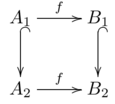
\includegraphics[scale=0.6]{master_master-1.png}
  \end{center}
  
  Then for $\Gamma$ closed conic in $B_2$ such that $N_f \cap \Gamma =
  \varnothing$ we have the following diagram commuting
  \begin{center}
    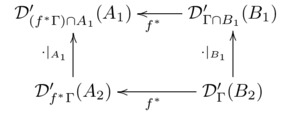
\includegraphics[scale=0.6]{master_master-2.png}
    
    
  \end{center}
  (here expressions like $X \cap \Gamma$ mean $\assign \{ ( x, \xi) \in \Gamma
  | x \in X \}$)
\end{lemma}

\begin{proof}
  First of all, we need to show that all maps in the second diagram make
  sense. The lowest horizontal is definitely so, as implied directly by
  hypothesis and fact \ref{holomorphicity-preserving:fact-pullback}. The
  vertical arrows also make sense by fact
  \ref{holomorphicity-preserving:fact-pullback}, as we note that for inclusion
  $\iota : X \longhookrightarrow Y$ the restriction $\mathcal{D}' ( Y)
  \rightarrow \mathcal{D}' ( X)$ can be seen as a pullback $\iota^{\ast}$.
  Moreover, for conic $\Gamma$ in $Y$ we have $\iota^{\ast} \Gamma = \Gamma
  \cap X$ just from the definition. Finally, the top horizontal arrow makes
  sense, as $f^{\ast} ( \Gamma \cap B_1) = ( f^{\ast} \Gamma) \cap A_1$ (by
  the slight abuse of notation, in the latter expression $f$ really stands for
  $f |_{A_1} : A_1 \rightarrow B_1$).
  
  Finally, the whole diagram commutes as it definitely does so when we start
  with an element of $C^{\infty} ( B_2) \subset \mathcal{D}'_{\Gamma} ( B_2)$,
  and then we can extend by continuity of pullback (fact
  \ref{holomorphicity-preserving:fact-pullback}) and approximation by smooth
  elements (fact \ref{holomorphicity-preserving:fact-p3}).
\end{proof}

\begin{lemma}
  \label{KR-normalization-recur:lem-pull-distrib-tensor}(``pullback and
  tensor's distributive law'') For $X_i, Y_i$ open subsets of Euclidian space
  for $i = 1, 2$ and $f_i : X_i \rightarrow Y_i$, $\Gamma_i$ conic closed in
  $Y_i$ such that $N_{f_i} \cap \Gamma_i = \varnothing$ and $u_i \in
  \mathcal{D}'_{\Gamma_i} ( Y_i)$, we have $N_{f_1 \times f_2} \cap ( \Gamma_1
  \otimes \Gamma_2) = \varnothing$ and $( f_1 \times f_2)^{\ast} ( u_1 \otimes
  u_2) = ( f_1^{\ast} u_1) \otimes ( f_2^{\ast} u_2)$.
\end{lemma}

\begin{proof}
  First of all, let us prove that $N_{f_1 \times f_2} \cap ( \Gamma_1 \otimes
  \Gamma_2) = \varnothing$. For this it suffices to show that $N_{f_1 \times
  f_2} = N_{f_1} \times N_{f_2}$. But the latter is clear from the definition
  of $N_f$ given in fact \ref{holomorphicity-preserving:fact-pullback}.
  
  Now, as the result is true for $u_i \in C^{\infty} ( Y_i)$, it holds in
  general by continuity of the pullback and tensor given by facts
  \ref{holomorphicity-preserving:fact-pullback} and
  \ref{holomorphicity-preserving:fact-p1} respectively, using approximation
  provided by fact \ref{holomorphicity-preserving:fact-p3}.
\end{proof}

\begin{lemma}
  \label{KR-normalization-recur:lem-mult-distrib-tensor}(``tensor and
  multiplication distributive law'') Let $\{ X_j \}_{j = 1, 2}$ be open
  subsets of Euclidean space and $\Gamma_i^{_j}$ closed conics in $X_j$ for $i
  = 1, 2$, such that for $j = 1, 2$, we have $( \Gamma_1^j \otimes \Gamma_2^j)
  \cap N_{\Delta_j} = \varnothing$ where $\Delta_j : X_j \rightarrow X_j
  \times X_j$ is diagonal embedding. Then for $u_i^j \in
  \mathcal{D}'_{\Gamma^{_j}_i} ( X_j)$ we have $( u_1^1 \otimes u_1^2) \cdot (
  u_2^1 \otimes u_2^2) = ( u_1^1 \cdot u_2^1) \otimes ( u_1^2 \otimes u_2^2)$,
  where $u \cdot v \assign \Delta^{\ast} ( u \otimes v)$.
\end{lemma}

\begin{proof}
  As $\Delta_{X_1 \times X_2} = \Delta_1 \times \Delta_2$, we have the chain
  of equalities
  \begin{eqnarray}
    & ( u_1^1 \otimes u_1^2) \cdot ( u_2^1 \otimes u_2^2) \assign \Delta_{X_1
    \times X_2}^{\ast} ( \{ u_1^1 \otimes u_1^2 \} \otimes \{ u_2^1 \otimes
    u_2^2 \}) = ( \Delta_1^{} \times \Delta_2)^{\ast} ( \{ u_1^1 \otimes u_1^2
    \} \otimes \{ u_2^1 \otimes u_2^2 \}) = &  \nonumber\\
    & = \Delta_1^{\ast} ( u_1^1 \otimes u_1^2) \otimes \Delta_2^{\ast} (
    u_2^1 \otimes u_2^2) = ( u_1^1 \cdot u_2^1) \otimes ( u_1^2 \otimes
    u_2^2), &  \nonumber
  \end{eqnarray}
  the third following from the lemma
  \ref{KR-normalization-recur:lem-pull-distrib-tensor}, and these end the
  proof.
\end{proof}

\begin{lemma}
  \label{KR-normalization-recur:lem-mult-smth}Assume for $U \subset
  \mathbbm{R}^n$ open that $f_i \in \mathcal{D}'_{\Gamma_i} ( U)$ for $i = 1,
  2$, such that $( \Gamma_1 \otimes \Gamma_2) \cap N_{\Delta} = \varnothing$
  (where $\Delta : U \rightarrow U \times U$ is a diganal embedding;
  $N_{\Delta}$ and $\Gamma_1 \otimes \Gamma_2$ are as in fact
  \ref{holomorphicity-preserving:fact-pullback} prop.
  \ref{holomorphicity-preserving:prop-tensor-holo} respectively). Let
  $\mathcal{D}' ( U) \ni h \assign \Delta^{\ast} ( f \otimes g)$ with pullback
  $\Delta^{\ast}$ being well-defined by facts
  \ref{holomorphicity-preserving:fact-p1} and
  \ref{holomorphicity-preserving:fact-pullback}. Then, if for $V \subset
  U$:open $f |_V \in C^{\infty} ( V)$, we have $h |_V = f |_V \cdot g |_V$ (in
  the sense of product of smooth function and distribution).
\end{lemma}

\begin{proof}
  As both tensor product and pullback commute with restriction (former follows
  by uniqueness part of fact \ref{holomorphicity-preserving:fact-tensor}; for
  latter, more precisely, we apply lemma
  \ref{KR-normalization-recur:lem-pull-comm-restr} with $( A_1, A_2) : = ( V,
  U)$, $( B_1, B_2) \assign ( V^2, U^2)$, $f \assign \Delta$ and $\Gamma
  \assign \Gamma_1 \otimes \Gamma_2$), we can assume $f \in C^{\infty} ( U)$
  from the outset. Then, fact \ref{holomorphicity-preserving:fact-p3} allows
  us to pick $C^{\infty} ( U) \ni g_j \rightarrow g$ in
  $\mathcal{D}'_{\Gamma_2} ( U)$. Then fact
  \ref{holomorphicity-preserving:fact-p1} tells us that $C^{\infty} ( U \times
  U) \ni f \otimes g_j \rightarrow f \otimes g$ \ in $\mathcal{D}'_{\Gamma_1
  \otimes \Gamma_2} ( U \times U)$ and consequently by fact
  \ref{holomorphicity-preserving:fact-pullback} $f \cdot g_j = \Delta^{\ast} (
  f \otimes g_j) \rightarrow \Delta^{\ast} ( f \otimes g)$. But then as $g_j
  \rightarrow g$ in $\mathcal{D}'_{\Gamma_2} ( U)$, hence $g_j \rightarrow g$
  in $\mathcal{D}' ( U)$, we have $f \cdot g_j \rightarrow f \cdot g$ with
  both sides in sense of product of smooth function and distribution, and
  since the sequence in $\mathcal{D}' ( U)$ can have at most one limit, we are
  done.
\end{proof}

\begin{lemma}
  \label{KR-normalization-recur:lem-mult-comm-pull}Let $U \subset
  \mathbbm{R}^n$ open, and for $i = 1, 2$ $\Gamma_i \subset U \times (
  \mathbbm{R}^n \backslash \{ 0 \})$ closed conic and $f_i \in
  \mathcal{D}'_{\Gamma_i} ( U)$, such that $N_{\Delta} \cap ( \Gamma_1 \otimes
  \Gamma_2) = \varnothing$. Suppose further that $\psi : V \rightarrow U$ is a
  diffeomorphism. Then $N_{\Delta} \cap ( \psi^{\ast} \Gamma_1 \otimes
  \psi^{\ast} \Gamma_2) = \varnothing$ and $\psi^{\ast} ( f_1 \cdot f_2) = (
  \psi^{\ast} f_1) \cdot ( \psi^{\ast} f_2)$ with product defined as in lemma
  \ref{KR-normalization-recur:lem-mult-distrib-tensor}.
\end{lemma}

\begin{proof}
  Let us first show that $N_{\Delta} \cap ( \psi^{\ast} \Gamma_1 \otimes
  \psi^{\ast} \Gamma_2) = \varnothing$. Indeed, suppose this happens, which
  implies that for some $U \times ( \mathbbm{R}^n \backslash \{ 0 \}) \ni ( x,
  \xi)$ we have $( x, \xi) \in \psi^{\ast} \Gamma_1$ and $( x, - \xi) \in
  \psi^{\ast} \Gamma_2$. This implies that $( f ( x), f' ( x)^{- T} \xi) \in
  \Gamma_1$ and $( f ( x), - f' ( x)^{- T} \xi) \in \Gamma_2$, hence
  $N_{\Delta} \cap ( \Gamma_1 \otimes \Gamma_2) \neq \varnothing$. This
  contradicts hypothesis and hence $N_{\Delta} \cap ( \psi^{\ast} \Gamma_1
  \otimes \psi^{\ast} \Gamma_2) = \varnothing$.
  
  The second statement follows by approximation by smooth functions (both
  pullback and tensor being continuous by facts
  \ref{holomorphicity-preserving:fact-pullback} and
  \ref{holomorphicity-preserving:fact-p1} respectively).
\end{proof}

\section{Setting and notations}\label{sec:def-n-nots}

\subsection{Groups $G \supset G'$ and their subgroups}

We fix $p, q \in \mathbbm{Z}_{\geq 1}$, $n \assign p + q$, $G \assign O (p +
1, q + 1)$ and $G' \assign O (p + 1, q + 1)_{e_{p + 1}} \assign \{g \in G|g
\cdot e_{p + 1} = e_{p + 1} \} \simeq O (p, q + 1)$. We shall also be
interested in the following
\begin{eqnarray}
  & M \assign \left\{ \left[ \begin{array}{ccc}
    \epsilon & 0 & 0\\
    0 & A & 0\\
    0 & 0 & \epsilon
  \end{array} \right] | A \in O (p, q), \hspace{0.75em} \epsilon = \pm 1
  \right\} \supset M^0 \assign \left\{ \left[ \begin{array}{ccc}
    1 & 0 & 0\\
    0 & A & 0\\
    0 & 0 & 1
  \end{array} \right] | A \in O (p, q), \hspace{0.75em} \epsilon = \pm 1
  \right\} &  \nonumber\\
  & N_+ \assign \left\{ n ( w) \assign n_+ ( w) \assign \left[
  \begin{array}{lll}
    1 - \frac{Q ( w)}{2} & - ( J w)^T & \frac{Q ( w)}{2}\\
    w & I_{p + q} & - w\\
    - \frac{Q ( w)}{2} & - ( J w)^T & 1 + \frac{Q ( w)}{2}
  \end{array} \right] | w \in \mathbbm{R}^{p, q} \right\} \simeq
  \mathbbm{R}^{p, q}  \label{def-n-nots:eq-N+} & \\
  & N_- \assign \left\{ n_- ( w) \assign \left[ \begin{array}{lll}
    1 - \frac{Q ( w)}{2} & - ( J w)^T & - \frac{Q ( w)}{2}\\
    w & I_{p + q} & w\\
    \frac{Q ( w)}{2} & ( J w)^T & 1 + \frac{Q ( w)}{2}
  \end{array} \right] | w \in \mathbbm{R}^{p, q} \right\} \simeq
  \mathbbm{R}^{p, q}  \label{def-n-nots:eq:N-} & \\
  & A \assign \{a (t) \assign \left[ \begin{array}{ccc}
    \cosh (t) & 0 & \sinh (t)\\
    0 & I_{p + q} & 0\\
    \sinh (t) & 0 & \cosh (t)
  \end{array} \right] |t \in \mathbbm{R}\} \simeq \mathbbm{R}. 
  \label{def-n-nots:eq-A} & 
\end{eqnarray}


Here $Q ( \cdot)$ denotes the \ $( p, q)$-quadratic form and $J$ is the
diagonal matrix with $p$ ``+1'' entries and $q$ ``-1'' entries. We also let
$M' \assign M \cap G'$, $N_{\pm}' \assign N_{\pm} \cap G' \simeq
\mathbbm{R}^{p - 1, q}$, $A' \assign A \cap G' = A$.

\begin{remark}
  $M, A, N_+ \subset G$ introduced above are closed subgroups of $G$ and
  similarly for $G'$. We will use $\mathfrak{a} \assign \tmop{Lie} ( A)$ and
  $\mathfrak{n}_{\pm} \assign \tmop{Lie} ( N_{\pm})$ notation for
  corresponding Lie algebras and similarly for $G'$.
\end{remark}

\begin{proposition}
  $G$ is a reductive group (of non-inner type) in the sense of
  {\cite{wallach1988real}} with $P \assign M A N_+ \subset G$ being a maximal
  parabolic subgroup of $G$ (here ``parabolic'' is in the sense of {\cite[sec.
  2.2]{wallach1988real}}). $P = M A N_+$ is a Langlands decomposition. In
  particular, multiplication $M \times A \times N_+ \rightarrow P$ is a
  diffeomorphism.
\end{proposition}

\begin{remark}
  Similar statement holds for $G' \supset P' \assign M' A' N_+' = P \cap G'$.
\end{remark}

\begin{proof}
  Follows by direct computations and the theory of reductive groups.
\end{proof}

\subsection{Degenerate principal series of $G$ and symmetry breaking
operators}

\begin{proposition}
  \label{def-n-nots:prop-degseries}For $\lambda \in
  \mathfrak{a}_{\mathbbm{C}}^{\ast} \simeq \mathbbm{C}$ and $\nu \simeq (
  \mathfrak{a}_{\mathbbm{C}}')^{\ast}$ fixed we have $G \times_P
  \mathbbm{C}_{\lambda} \assign ( G \times \mathbbm{C}) / \sim$ and $G'
  \times_{P'} \mathbbm{C}_{\nu} \assign ( G' \times \mathbbm{C}) / \sim'$
  being smooth vector bundles over $G / P$ and $G' / P'$ respectively. Here
  the equivalence relation is defined as $( g, x) \sim ( g_{\sim}, x_{\sim})$
  iff for some $p \in P$ we have $g_{\sim} = g p$ and $x_{\sim} = \lambda (
  p^{- 1}) x$ with $\lambda : G \rightarrow \mathbbm{C}^{\times}$ defined as a
  composition $G \simeq M \times A \times N_+ \rightarrow A \simeq
  \mathfrak{a} \ni H \mapsto \exp ( \lambda ( H)) \in \mathbbm{C}^{\times}$.
  Similarly, $\sim'$ is defined.
  
  We will let $I ( \lambda)$ and $J ( \nu)$ denote the space of smooth
  sections of $G \times_P \mathbbm{C}_{\lambda}$ and $G' \times_{P'}
  \mathbbm{C}_{\nu}$ respectively. Then $I ( \lambda)$ and $J ( \nu)$ have the
  structure of Frechet spaces and are Frechet representations of $G$ and $G'$
  respectively.
\end{proposition}

\begin{remark}
  Thesee $I ( \lambda)$ and $J ( \nu)$ are particular instances of
  \tmtextit{degenerate principal series}.
\end{remark}

\begin{proof}
  The fact that $G \times_P \mathbbm{C}_{\lambda}$ and $G' \times_{P'}
  \mathbbm{C}_{\nu}$ so defined are vector bundles is evident. The Frechet
  structure and continuity of $G$ (or $G'$) action are also evident.
\end{proof}

Having this setup, we can strictly formulate the main question we are trying
to solve:

{\noindent}\tmtextbf{Question. }\tmtextit{For given pair $( \lambda, \nu) \in
\mathfrak{a}_{\mathbbm{C}}^{\ast} \times (
\mathfrak{a}'_{\mathbbm{C}})^{\ast}$ explicitly describe the vector space of
$\tmop{Hom}_{G'} ( I ( \lambda), J ( \nu))$. In particular, find the explicit
form of a basis elements.}{\hspace*{\fill}}{\medskip}

\begin{remark}
  We will call the members of $\tmop{Hom}_{G'} ( I ( \lambda), J ( \nu))$ by
  the name \tmtextit{symmetry breaking operators} or SBOs for short.
\end{remark}

\subsection{Another model for degenerate principal series representations}

As the degenerate principal series we are interested in are smooth sections of
the vector bundle over $G / P$ (and $G' / P'$), it is naturally necessary to
learn a bit more about the geometry of these. For this we will need a
different model of $G \curvearrowright G / P$ action.

\begin{proposition}
  \label{def-n-nots:prop-ximodel}Set $\mathbbm{R}^{p + 1, q + 1} \supset \Xi
  \assign \{ (x, y) \in \mathbbm{R}^{p + 1, q + 1} \setminus \{ 0 \} | | x | =
  | y | \}$. $\Xi$ is invariant under left multiplication by an elements of
  $G$. The centralizer of $p_+ \assign ( 1, 0_{p + q}, 1) \in \Xi$ equals to
  $M_{}^0 N_+$.
  
  This induces action $G \curvearrowright \Xi /\mathbbm{R}^{\times} \simeq (
  \mathbbm{S}^p \times \mathbbm{S}^q) / \{ \pm 1 \}$. The centralizer of $p_+
  \mathbbm{R}^{\times} \in \Xi /\mathbbm{R}^{\times}$ is then equal to $P$.
\end{proposition}

\begin{remark}
  Here and in subsequent we will use notation $0_n$ or $1_n$ to denote $n$
  consecutive zeros or ones respectively.
\end{remark}

\begin{proof}
  Direct computations.
\end{proof}

\begin{lemma}
  \label{k-finite:lem-homocone}Let $\Xi \assign \{ ( x, y) \in \mathbbm{R}^{p
  + 1, q + 1} |  | x |_{p + 1} = | y |_{q + 1} \neq 0 \}$ and $\Gamma_{\Xi}
  \assign \{ ( x, \xi) \in T^{\nobracket \ast \nobracket}_{} ( \Xi) | x \perp
  \xi \}$ closed conic in $\Xi$. Then under a diffeomorphism $\Xi \simeq
  \mathbbm{S}^p \times \mathbbm{S}^q \times \mathbbm{R}_{> 0}$, $\Gamma_{\Xi}$
  is pulled back to $\Gamma_1 \otimes \varnothing$, where $\Gamma_1$ is full
  cone in $\mathbbm{S}^p \times \mathbbm{S}^q$. Moreover, for any $f \in
  \mathcal{D}' ( \Xi)$ homogeneous we have $f \in \mathcal{D}'_{\Gamma_{\Xi}}
  ( \Xi)$.
\end{lemma}

\begin{proof}
  The proof of the first assertion is purely computational and will be
  omitted. The second in turn follows from the fact that any homogeneous $f
  \in \mathcal{D}' ( \Xi)$ of degree $a$ when pulled back to $\mathbbm{S}^p
  \times \mathbbm{S}^q \times \mathbbm{R}_{> 0}$ will become $g \otimes s^a$
  with some $g \in \mathcal{D}' ( \mathbbm{S}^p \times \mathbbm{S}^q)$. Then,
  the desired conclusion is granted by fact
  \ref{holomorphicity-preserving:fact-p1}.
\end{proof}

\begin{lemma}
  \label{k-finite:lem-claim1-aux}Let $\psi : \mathfrak{n}_- \simeq
  \mathbbm{R}^{p, q} \ni v \mapsto ( 1 - Q ( v), 2 v, 1 + Q ( v)) \in \Xi$ be
  an embedding. Then we have that $\mathfrak{n}_- \times \mathbbm{R}^{\times}
  \ni ( x, t) \mapsto \psi ( x) t \in \Xi$ is a diffemorphism with an open
  image, that we will call $\mathfrak{n}_- \mathbbm{R}^{\times} \subseteq
  \Xi$.
\end{lemma}

\begin{proof}
  Again, this is computational and the proof will be omitted.
\end{proof}

\begin{lemma}
  \label{k-finite:lem-restriction-to-N}For $\psi : \mathbbm{R}^{p, q}
  \rightarrow \Xi$ and $\Gamma_{\Xi}$ as in lemmas
  \ref{k-finite:lem-claim1-aux} and \ref{k-finite:lem-homocone} respectively,
  we have $N_{\psi} \cap \Gamma_{\Xi} = \varnothing .$
\end{lemma}

\begin{proof}
  So let's take arbitrary $w \in \mathbbm{R}^{p, q}$ fixed and unfolding
  definitions, what we need to show, is that if nonzero $\xi \in T_{\psi (
  w)}^{\ast} \Xi$ is perpendicular to $\psi ( w)$, then $D \psi ( w)^T \xi
  \neq 0$. Now, writing $\xi = : ( \alpha, u, \beta) \in \mathbbm{R} \times
  \mathbbm{R}^{p, q} \times \mathbbm{R}$ the conditions $\xi \in T_{\psi ( w)}
  \Xi$ and $\xi \perp \psi ( w)$ are written as (note that the perpendicular
  to $\Xi$ at $x$ is given by $\tilde{J} x$, where $\tilde{J}$ is diagonal
  matrix of $p + 1$ -1's followed by $q + 1$ 1's): $( 1 - Q ( w)) \alpha + 2
  \langle J w, u \rangle - \beta ( 1 + Q ( w)) = 0$ and $( 1 - Q ( w)) \alpha
  + 2 \langle w, u \rangle + \beta ( 1 + Q ( w)) = 0$ respectively (here
  $\langle \cdot, \cdot \rangle$ denotes inner product on $\mathbbm{R}^{p +
  q}$).
  
  Now, assuming that $D \psi ( w)^T \xi = 0$, in order to show that $\xi = 0$
  and thus reach a contradiction, this additionally gives us $J w ( \beta -
  \alpha) + u = 0$ (here $J$ is diagonal matrix with first $p$ items +1 and
  then $q$ items -1) and substituting this into
  \begin{eqnarray}
    & \left\{ \begin{array}{l}
      ( 1 - Q ( w)) \alpha + 2 \langle J w, u \rangle - \beta ( 1 + Q ( w)) =
      0\\
      ( 1 - Q ( w)) \alpha + 2 \langle w, u \rangle + \beta ( 1 + Q ( w)) = 0
    \end{array} \right. &  \nonumber
  \end{eqnarray}
  gives us
  \[ \left\{ \begin{array}{l}
       ( 1 - Q ( w)) \alpha + 2 ( \alpha - \beta) \langle J w, J w \rangle -
       \beta ( 1 + Q ( w)) = 0\\
       ( 1 - Q ( w)) \alpha + ( \alpha - \beta) 2 \langle w, J w \rangle +
       \beta ( 1 + Q ( w)) = 0
     \end{array} \right. \]
  or equivalently (note that $\langle J w, w \rangle = Q ( w)$)
  \[ \left\{ \begin{array}{l}
       ( \alpha - \beta) ( 1 + 2 \langle w, w \rangle) - Q ( w) ( \alpha +
       \beta) = 0\\
       ( \alpha + \beta) + Q ( w) ( \alpha - \beta) = 0
     \end{array} \right. \]
  and seeing this as linear system in $\{ \alpha - \beta, \alpha + \beta \}$,
  we see that the determinant is $1 + 2 | w |^2 + Q^2 > 0$, hence $\alpha -
  \beta = \alpha + \beta = 0 \Rightarrow \alpha = \beta = 0 \Rightarrow u = 0$
  and thus $\xi = 0$.
\end{proof}

\begin{lemma}
  \label{k-finite:lem-claim1-aux-2} For $U \subset \mathbbm{R}^{p, q}$ open we
  let $U\mathbbm{R}^{\times}$ be the image of $U$ under $U \times
  \mathbbm{R}^{\times} \ni ( x, t) \mapsto \psi ( x) \cdot t \in \Xi$.With a
  diffeomorphism $U \times \mathbbm{R}^{\times} \simeq U\mathbbm{R}^{\times}$
  induced by that of lemma \ref{k-finite:lem-claim1-aux}, $f \in
  \mathcal{D}'_a ( U\mathbbm{R}^{\times})$ is pulled back to an element $f
  |_{\psi ( U)} \otimes | s |^a \in \mathcal{D}' ( \mathfrak{n}_- \times
  \mathbbm{R}^{\times})$ and conversely every element of this form is pulled
  back to an element of $\mathcal{D}'_a ( U\mathbbm{R}^{\times}) .$
\end{lemma}

\begin{remark}
  Note that restriction is well-defined in the light of lemmas
  \ref{k-finite:lem-homocone} and \ref{k-finite:lem-restriction-to-N}.
\end{remark}

\begin{proof}
  We assume $U =\mathfrak{n}_-$, the general statement being proven by the
  same technique. The converse statement is clear, so we just need to prove
  the direct one. Note that the commutative diagram
  
  \begin{center}
    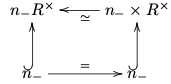
\includegraphics[scale=0.6]{master_master-3.png}
  \end{center}
  
  (with right inclusion being $x \mapsto x \times \{ 1 \}$) implies the
  commutative diagram
  
  \begin{center}
    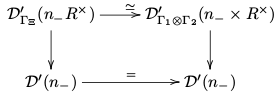
\includegraphics[scale=0.6]{master_master-4.png}
  \end{center}
  
  with restrictions well-defined by lemmas \ref{k-finite:lem-restriction-to-N}
  and \ref{k-finite:lem-homocone} (with $\Gamma_{1, 2}$ as in lemma
  \ref{k-finite:lem-homocone}).
  
  Now, given $f \in \mathcal{D}'_a ( \mathfrak{n}_- \mathbbm{R}^{\times})$ one
  sees (multiplying it by smooth function of degree $- a$ and using the fact
  \ref{fact:sing-q-4}) that $f$ is pulled back to $g \otimes | s |^a$ with $g
  \in \mathcal{D}' ( \mathfrak{n}_-)$. Now, approximating $g$ by smooth and
  using continuity of pullback and tensor, one sees that $g$ equals to the
  restriction of the $g \otimes | s |^a$, and hence $g$ equals to the
  resctriction of $f$ due to the commutativity of the latter diagram.
\end{proof}

\begin{lemma}
  \label{k-finite:lem-claim1}For $f \in \mathcal{D}' ( U)$ (with $U \subset
  \mathbbm{R}^{p, q}$:open) and $a \in \mathbbm{C}$ there is unique $f^a \in
  \mathcal{D}'_a ( U\mathbbm{R}^{\times})$ such that $f^a |_{\psi ( U)} = f$.
  Map $f \mapsto f^a$ is continuous for fixed $a \in \mathbbm{C}$. Moreover,
  if for $\Omega \subset \mathbbm{C}^n$ open, $a ( \cdot)$ holomorphic on
  $\Omega$ and $f_{\mu} \in \mathcal{D}' ( U)$ holomorphic in $\mu \in
  \Omega$, we have $( f_{\mu})^{a ( \mu)}$ being holomorphic in
  $\mathcal{D}'_{\Gamma_{\Xi}}$ (as in definition
  \ref{holomorphicity-preserving:def-holo-in-DG}).
\end{lemma}

\begin{proof}
  Again, we assume $U =\mathfrak{n}_-$, the general statement being handled in
  the same way. Lemma \ref{k-finite:lem-claim1-aux-2} immediately implies the
  uniqueness part. The existence follows by taking $f \otimes | s |^a \in
  \mathcal{D}' ( \mathfrak{n}_- \times \mathbbm{R}^{\times})$ for $f \in
  \mathcal{D}' ( \mathfrak{n}_-)$ and then pulling back to some $f^a \in
  \mathcal{D}' ( \mathfrak{n}_- \mathbbm{R}^{\times})$. It will then follow
  that $f^a |_{\psi ( \mathfrak{n}_-)} = f$ by continuity of pullback and
  tensor product (facts \ref{holomorphicity-preserving:fact-pullback} and
  \ref{holomorphicity-preserving:fact-p1} respectively) and approximation of
  $f \in \mathcal{D}' ( \mathfrak{n}_-)$ by smooth elements.
  
  The continuity of $f \mapsto f^a$ follows by continuity of pullback and
  tensor. Holomorphicity follows by propositions
  \ref{holomorphicity-preserving:prop-pullback-holo} and
  \ref{holomorphicity-preserving:prop-tensor-holo} (in particular
  holomorphicity of $| s |^{a ( \mu)}$ in $\mathcal{D}'_{\varnothing} (
  \mathbbm{R}\backslash \{ 0 \})$ is given by lemma
  \ref{k-finite:lem-abs-is-holo} and note that multiplication $m :
  \mathfrak{n}_- \times \mathbbm{R}^{^{} \times} \ni ( v, t) \mapsto t \cdot
  \psi ( v) \in \Xi$ pulls $\Gamma_{\Xi}$ to $\Gamma \otimes \varnothing$ with
  $\Gamma$ being the full cone in $\mathfrak{n}_-$).
\end{proof}

\begin{lemma}
  \label{k-finite:lem-restriction-to-S}For $\psi_S : \mathbbm{S}^p \times
  \mathbbm{S}^q \hookrightarrow \Xi$ embedding we have $\Gamma_{\Xi} \cap
  N_{\psi_S} = \varnothing$. Moreover, under $\Xi \simeq \mathbbm{S}^p \times
  \mathbbm{S}^q \times \mathbbm{R}_{> 0}$ every homogeneous $f \in
  \mathcal{D}'_a ( \Xi)$ is pulled back to $f |_{\mathbbm{S}^p \times
  \mathbbm{S}^q} \otimes | u |^a$ with $f |_{\mathbbm{S}^p \times
  \mathbbm{S}^q} \in \mathcal{D}' ( \mathbbm{S}^p \times \mathbbm{S}^q)$:even
  and conversely every function of this kind is homogeneous in $\Xi$ of degree
  $a$.
\end{lemma}

\begin{proof}
  $\Gamma_{\Xi} \cap N_{\psi_S} = \varnothing$ is seen immediately, as
  $N_{\psi_S}$ is the normal bundle of $\mathbbm{S}^p \times \mathbbm{S}^q
  \subset \Xi$. The ``conversely'' part is also seen in the light of $\Xi
  \simeq \mathbbm{S}^p \times \mathbbm{S}^q \times \mathbbm{R}_{> 0}$
  diffeomorphism, so it remains to show that every homogeneous $f \in
  \mathcal{D}'_a ( \Xi)$ is pulled back to $f |_{\mathbbm{S}^p \times
  \mathbbm{S}^q} \otimes | u |^a$ with $f |_{\mathbbm{S}^p \times
  \mathbbm{S}^q} \in \mathcal{D}' ( \mathbbm{S}^p \times \mathbbm{S}^q)$:even
  under $\Xi \simeq \mathbbm{S}^p \times \mathbbm{S}^q \times \mathbbm{R}_{>
  0}$. As diffeomorphisms and inclusions induce the commutative diagram
  \begin{center}
    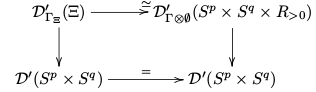
\includegraphics[scale=0.6]{master_master-5.png}
  \end{center}
  and we see (multiplying $f \in \mathcal{D}'_a ( \Xi)$ by smooth homogeneous
  function of order $- a$ and using fact \ref{fact:sing-q-4}, one sees that
  $f$ is pulled back to $g \otimes | u |^a$ with $g \in \mathcal{D}' (
  \mathbbm{S}^p \times \mathbbm{S}^q)$ even. Finally, aprroximating $g$ with
  even smooth elements of $C^{\infty} ( \mathbbm{S}^p \times \mathbbm{S}^q)$,
  we see that commutativity of above diagram and continuity of pullback and
  tensor imply that $g = f |_{\mathbbm{S}^p \times \mathbbm{S}^q}$.
\end{proof}

\begin{lemma}
  \label{k-finite:lem-holo-easy}Suppose $K_{\mu} \in \mathcal{D}'_{\lambda (
  \mu)} ( \Xi)$ is holomorphic in $\mu \in \Omega \subset \mathbbm{C}^n$ with
  $\lambda ( \cdot)$ holomorphic on $\Omega$. Then $K_{\mu}$ is holomorphic in
  $\mathcal{D}'_{\Gamma_{\Xi}} ( \Xi)$.
\end{lemma}

\begin{proof}
  Mulitplication induces the diffeomorphism $( \mathbbm{S}^p \times
  \mathbbm{S}^q) \times \mathbbm{R}_{> 0} \simeq U$. Lemma
  \ref{k-finite:lem-restriction-to-S} implies that under this diffeomorphism
  $K_{\mu}$ is pulled back to $F_{\mu} \otimes s^{\lambda ( \mu)}$. As lemma
  \ref{k-finite:lem-abs-is-holo} implies that $s^{- \lambda ( \mu)} \in
  \mathcal{D}' ( \mathbbm{R}_{> 0})$ is holomorphic in
  $\mathcal{D}'_{\varnothing}$, holomorphicity of distribution product implies
  that $F_{\mu} \otimes 1$ is holomorphic. Hence, so is $F_{\mu} \in
  \mathcal{D}' ( \mathbbm{S}^p \times \mathbbm{S}^q)$ and then holomorphicity
  of tensor product implies the desired conclusion.
\end{proof}

\begin{lemma}
  \label{k-finite:lem-compat-N-aux}The following holds:
  \begin{enumerate}
    \item For $\xi \in \Xi$ we have $\xi \in \mathfrak{n}_-
    \mathbbm{R}^{\times}\prime \Leftrightarrow \xi_1 + \xi_{p + q + 2} \neq 0$
    
    \item For $b, x \in \mathbbm{R}^{p, q}$ with $b_p = 0$ we have $n_+ ( b)
    \psi ( x) \in \mathfrak{n}_- \mathbbm{R}^{\times} \Leftrightarrow c_b ( x)
    \assign 1 - 2 Q ( b, x) + Q ( b) Q ( x) \neq 0.$ And if these hold, then
    $n_+ ( b) \psi ( x) = c_b ( x) \psi ( ( x - Q ( x) b) / c_b ( x))$.
  \end{enumerate}
\end{lemma}

\begin{proof}
  We first prove the first item. As ``$\Rightarrow$'' direction is clear, we
  only need to show the converse. \ Assuming that $\xi_1 + \xi_{p + q + 2}
  \neq 0$, we let $t \assign ( \xi_{p + q + 2} + \xi_1) / 2$ and
  $\mathbbm{R}^{p, q} \ni b \assign ( \xi_2, \xi_3, \ldots, \xi_{p + q + 1}) /
  2 t$. It is then a matter of direct calculations to see that $\xi = t \cdot
  \psi ( b)$. This proves the first item.
  
  Now it remains to show the second. If $c_b ( x) \neq 0$, then $n_+ ( b) \psi
  ( x) = c_b ( x) \psi ( ( x - Q ( x) b) / c_b ( x))$ by direct computations
  (with $n ( \cdot)$ as in $( \ref{def-n-nots:eq-N+})$), so it suffices to
  show that $n_+ ( b) \psi ( x) \in \mathfrak{n}_- \mathbbm{R}^{\times}$
  implies that $c_b ( x) \neq 0$. But this is again matter of direct
  calculations to see that for $\xi \assign n_+ ( b) \psi ( x)$ we have $\xi_1
  + \xi_{p + q + 2} = c_b ( x)$ and then the conclusion is implied by the
  first item.
\end{proof}

\begin{lemma}
  \label{k-finite:lem-restr-opendense}Consider an embedding $\psi_{N
  \rightarrow S} : \mathfrak{n}_- \simeq \mathbbm{R}^{p, q} \ni x \mapsto \pi
  ( 1 - Q ( x), 2 x, 1 + Q ( x)) / \sqrt{R} \in \mathbbm{S}^p \times
  \mathbbm{S}^q$ (here $C^{\infty} ( \mathbbm{R}^{p, q}) \ni R$ is given in
  bipolar coordinates as $R ( r, s) \assign ( 1 - r^2 + s^2)^2 + 4 r^2$)). We
  let $\psi'_{N \rightarrow S}$ denote restriction of $\psi_{N \rightarrow S}$
  to $\{ x \in \mathbbm{R}^{p, q} \backslash \{ 0 \} | Q ( x) = 0 \}$. Then
  $\psi'_{N \rightarrow S} : \{ x \in \mathbbm{R}^{p, q} \backslash \{ 0 \} |
  Q ( x) = 0 \} \rightarrow \{ ( \xi, \eta) \in \mathbbm{S}^p \times
  \mathbbm{S}^q | \xi_1 = \eta_{q + 1} \}$ is an embedding. Moreover, $\pm
  \psi'_{N \rightarrow S} ( \{ x \in \mathbbm{R}^{p, q} \backslash \{ 0 \} | Q
  ( x) = 0 \}) \subset \{ ( \xi, \eta) \in \mathbbm{S}^p \times \mathbbm{S}^q
  | \xi_1 = \eta_{q + 1} \}$ is dense.
\end{lemma}

\begin{proof}
  It is clear that for every $x \in \mathbbm{R}^{p, q}$ with $Q ( x) = 0$ we
  have $\psi_{N \rightarrow S} ( x) \in \{ ( \xi, \eta) \in \mathbbm{S}^p
  \times \mathbbm{S}^q | \xi_1 = \eta_{q + 1} \}$. Then, smoothness of
  $\psi_{N \rightarrow S}'$ is readily given by {\cite[thm.
  1.32]{warner1971foundations}}. The fact that $\psi_{N \rightarrow S}'$ is an
  embedding follows from the fact that $\psi_{N \rightarrow S}'$ is an
  embedding when seen as $\{ x \in \mathbbm{R}^{p, q} \backslash \{ 0 \} | Q (
  x) = 0 \} \rightarrow \mathbbm{S}^p \times \mathbbm{S}^q$ map (hence,
  $\psi_{N \rightarrow S}'$ is an injective immersion) and that both domain
  and target of $\psi_{N \rightarrow S}'$ are $p + q - 1$-dimensional
  manifolds (hence, $\psi_{N \rightarrow S}'$ is an open map, hence
  homeomorphism into).
  
  Finally, we show that $\pm \psi'_{N \rightarrow S} ( \{ x \in
  \mathbbm{R}^{p, q} \backslash \{ 0 \} | Q ( x) = 0 \}) \subset \{ ( \xi,
  \eta) \in \mathbbm{S}^p \times \mathbbm{S}^q | \xi_1 = \eta_{q + 1} \}$ is
  dense. For this it suffices to show that image of $\psi : \{ x \in
  \mathbbm{R}^{p, q} \backslash \{ 0 \} | Q ( x) = 0 \} \ni x \mapsto ( 1 - Q
  ( x), 2 x, 1 + Q ( x)) \mathbbm{R}^{\times} \in \Xi /\mathbbm{R}^{\times}$
  equals to $\{ ( \xi_1, \xi', \xi_{p + q + 2}) \mathbbm{R}^{\times} \in \Xi
  /\mathbbm{R}^{\times} | \xi_1 + \xi_{p + q + 2} \neq 0, \xi_1 - \xi_{p + q +
  2} = 0, \xi' \neq 0 \}$. The $\subseteq$ is obvious. $\supseteq$ is seen by
  direct computations, as we just take $x \assign \xi' / 2 \xi_1$.
\end{proof}

\section{Double coset decomposition $P' \backslash G /
P$}\label{sec:doublePGP}

The purpose of this section is to explicitly describe double coset
decomposition $P' \backslash G / P$ and to show that $P N_- P' = G$ equality
holds.

\subsection{Main results}

\begin{proposition}
  \label{doublePGP:prop-orbitdeco}For $p, q \geqslant 1$ the action $P'
  \curvearrowright G / P \simeq \Xi /\mathbbm{R}^{\times} \simeq (
  \mathbbm{S}^p \times \mathbbm{S}^q) / \{ \pm \}$ has the following orbit
  decomposition:
  \begin{eqnarray}
    & \left\{ \begin{array}{ll}
      \{ x_{p + 1} \neq 0, x_1 \neq y_{q + 1} \} \sqcup \{ x_{p + 1} = 0, x_1
      \neq y_{q + 1} \} \sqcup \{ x_{p + 1} \neq 0, x_1 = y_{q + 1} \} \sqcup
      \{ \pm ( 1, 0_{p + q}, 1) \}, & p = 1\\
      \{ x_{p + 1} \neq 0, x_1 \neq y_{q + 1} \} \sqcup \{ x_{p + 1} = 0, x_1
      \neq y_{q + 1} \} \sqcup \{ x_{p + 1} \neq 0, x_1 = y_{q + 1} \} \sqcup
      & \\
      \sqcup \{ ( 1, 0_{p + q}, 1) \} \sqcup \{ x_{p + 1} = 0, x_1 = y_{q + 1}
      \} \backslash \{ \pm ( 1, 0_{p + q}, 1) \}, & p > 1
    \end{array} \right. = &  \nonumber\\
    & = \left\{ \begin{array}{ll}
      P' ( 0_p, 1, 0_q, 1) \sqcup P' ( 1, 0_{p + q}, - 1) \sqcup P' ( 0_p, 1,
      1, 0_q) \sqcup P' ( 1, 0_{p + q}, 1), & p = 1\\
      P' ( 0_p, 1, 0_q, 1) \sqcup P' ( 1, 0_{p + q}, - 1) \sqcup P' ( 0_p, 1,
      1, 0_q) \sqcup P' ( 1, 0_{p + q}, 1) \sqcup P' ( 0_{p - 1}, 1, 0, 1,
      0_q), & p > 1
    \end{array} \right. &  \nonumber
  \end{eqnarray}
  here, for example $\{ x_{p + 1} \neq 0, x_1 \neq y_{q + 1} \} \assign \{ (
  x, y) \in \mathbbm{S}^p \times \mathbbm{S}^q | x_{p + 1} \neq 0, x_1 \neq
  y_{q + 1} \} / \{ \pm \}$.
\end{proposition}

\begin{proposition}
  \label{doublePGP:prop-pullback-of-orbits}For $\psi : \mathbbm{R}^{p, q} \ni
  x \mapsto n_- ( w) ( 1, 0_{p + q}, 1) \mathbbm{R}^{\times} \in \Xi
  /\mathbbm{R}^{\times}$ with $n_- ( \cdot)$ as in (\ref{def-n-nots:eq:N-}) we
  have:
  \begin{eqnarray}
    & \psi ( w) \in \{ x_{p + 1} \neq 0, x_1 \neq y_{q + 1} \}
    \Leftrightarrow Q ( w) \neq 0 \hspace{1em} \tmop{and} \hspace{1em} w_p
    \neq 0 &  \nonumber\\
    & \psi ( w) \in \{ x_{p + 1} = 0, x_1 \neq y_{q + 1} \} \Leftrightarrow Q
    ( w) \neq 0 \hspace{1em} \tmop{and} \hspace{1em} w_p = 0 &  \nonumber\\
    & \psi ( w) \in \{ x_{p + 1} \neq 0, x_1 = y_{q + 1} \} \Leftrightarrow Q
    ( w) = 0 \hspace{1em} \tmop{and} \hspace{1em} w_p \neq 0 &  \nonumber\\
    & \psi ( w) \in \{ ( 1, 0_{p + q}, 1) \} \Leftrightarrow w = 0 & 
    \nonumber\\
    & \psi ( w) \in \{ x_{p + 1} = 0, x_1 = y_{q + 1} \} \backslash \{ \pm (
    1, 0_{p + q}, 1) \} \Leftrightarrow Q ( w) = 0 \nocomma, w_p \neq 0
    \hspace{1em} \tmop{and} \hspace{1em} w \neq 0 &  \nonumber
  \end{eqnarray}
  here, for example $\{ x_{p + 1} \neq 0, x_1 \neq y_{q + 1} \} \assign \{ (
  x, y) \in \mathbbm{S}^p \times \mathbbm{S}^q | x_{p + 1} \neq 0, x_1 \neq
  y_{q + 1} \} / \{ \pm \}$ and $Q$ denotes the quadratic $( p, q)$-form.
\end{proposition}

\begin{remark}
  It is easy to see that $\psi : \mathbbm{R}^{p, q} \rightarrow \Xi
  /\mathbbm{R}^{\times}$ is in fact an embedding.
\end{remark}

\begin{proposition}
  \label{doublePGP:prop-pnp}$P' N_- P = G$.
\end{proposition}

\subsection{Auxiliary lemmas}

\begin{lemma}
  \label{doublePGP:lem-comput}For $( v, w) \in \mathbbm{R}^{p, q}$ with $v_p =
  0$ and $t \in \mathbbm{R}$ let
  \begin{eqnarray}
    & n ( w) \assign \left[ \begin{array}{cccc}
      1 - \frac{| v |^2 - | w |^2}{2} & - v^T & w^T & \frac{| v |^2 - | w
      |^2}{2}\\
      v & I_p & 0 & - v\\
      w & 0 & I_q & - w\\
      - \frac{| v |^2 - | w |^2}{2} & - v^T & w^T & 1 + \frac{| v |^2 - | w
      |^2}{2}
    \end{array} \right] \in N_+' &  \nonumber\\
    & a ( t) \assign \left[ \begin{array}{ccc}
      \cosh (t) & 0 & \sinh (t)\\
      0 & I_{p + q} & 0\\
      \sinh (t) & 0 & \cosh (t)
    \end{array} \right] \in A' &  \nonumber\\
    &  &  \nonumber
  \end{eqnarray}
  be arbitrary elements of $N_+'$ and $A'$ respectively. And let $l_1 : (
  \mathbbm{S}^p \times \mathbbm{S}^q) / \{ \pm \} \ni \pm ( x, y) \mapsto \pm
  ( x_1 - y_{q + 1}) \in \mathbbm{R}/ \{ \pm \}$ and $l_2 : ( \mathbbm{S}^p
  \times \mathbbm{S}^q) / \{ \pm \} \ni \pm ( x, y) \mapsto \pm x_{p + 1} \in
  \mathbbm{R}/ \{ \pm \}$.
  
  Then for $p \in ( \mathbbm{S}^p \times \mathbbm{S}^q) / \{ \pm \}$ we have
  $l_i ( n ( w) \cdot p) = l_i ( a ( t) \cdot p) = l_i ( p)$ for $i = 1, 2$.
\end{lemma}

\begin{proof}
  This is directly seen, as one observes that for $( x, y) \in \mathbbm{S}^p
  \times \mathbbm{S}^q$ and $n ( w) ( x, y) = : ( x', y')$, $a ( t) ( x, y) =
  : ( x'', y'')$ we have $x_{p + 1}' = x_{p + 1}'' = x_{p + 1}$, $x'_1 - y_{q
  + 1}' = x_1 - y_{q + 1}$ and $x_1'' - y_{q + 1}'' = ( \cosh ( t) - \sinh (
  t)) ( x_1 - y_{q + 1}) = e^{- t} ( x_1 - y_{q + 1})$.
\end{proof}

\begin{lemma}
  \label{doublePGP:lem-zerocolumn}Let $a, b \in \mathbbm{Z}_{\geqslant 1}$ $H
  \assign O ( a, b)$ and $H' \assign \{g \in H|g \cdot e_a = e_a \}$. Then
  every element of $H'$ has its $a$-th row and column equal to $e_a$.
\end{lemma}

\begin{proof}
  For this we simply note that for elements of $x \in O ( a, b)$ we have $x^{-
  T} = \tmop{Ad} ( I_{a, b}) x$ (where $I_{a, b}$ is diagonal matrix with
  first $a$ +1's and then $b$ -1's). Hence, $H'$ is closed under
  transposition. Therefore, not only every element of $H'$ has it's $a$-th row
  equal to $e_a$ (as implied by $g \cdot e_a = e_a$ condition), but also
  $a$-th column equal to $e_a$.
\end{proof}

\begin{lemma}
  \label{doublePGP:lem-Gp-act-Xi}Let $a, b \in \mathbbm{Z}_{\geqslant 0}$ with
  $b \geqslant 1$ and $a \geqslant 2$. Let further $H \assign O ( a, b)$ and
  $H' \assign \{g \in H|g \cdot e_a = e_a \}$. Then $H' \curvearrowright
  \Xi^{a, b} \cap \{ x_a = 0 \}$ is transitive, where $\mathbbm{R}^{a, b}
  \supset \Xi^{a, b} \assign \{ ( x, y) \in \mathbbm{R}^{a, b} \backslash \{ 0
  \} |  | x | = | y | \}$.
\end{lemma}

\begin{proof}
  We first show that this action is well-defined. The lemma
  \ref{doublePGP:lem-zerocolumn} implies that $\{ x_a = 0 \}$ is
  $H'$-invariant and that the action is well-defined. We then show the
  transitiveness.
  
  As was shown above, every element of $H'$ has its $a$-th row and column
  equal to $e_a$. From this one directly sees (using blockwise matrix
  multiplication) that if we let $\pi ( g)$ denote the $g \in H$ with $a$-th
  row and column crossed out, then it induces $\pi : H' \rightarrow O ( a - 1,
  b)$ is a group isomorphism (fact that $\pi ( H') = O ( a - 1, b)$ is seen
  directly from the definition $X I_{s, t} = I_{s, t} X$ for an element $X$ of
  $O ( s, t)$ for $s, t \geqslant 1$).
  
  It is then clearly seen that for a diffeomorphism $\pi : \Xi^{a, b} \cap \{
  x_a = 0 \} \rightarrow \Xi^{a - 1, b}$ given by removal of $a$-th coordint
  we have $\pi ( g \cdot x) = \pi ( g) \cdot \pi ( x)$ for $( g, x) \in H'
  \times ( \Xi^{a, b} \cap \{ x_a = 0 \})$. Hence, it suffices to show that $O
  ( a - 1, b) \curvearrowright \Xi^{a - 1, b}$ is transitive. But this is
  true, as for arbitrary $( x, y) \in \Xi^{a - 1, b}$ we can use elements of
  $O ( a - 1) \times O ( b)$ to bring it to the form $( \alpha, 0_{a + b - 3},
  \alpha)$ with $\alpha > 1$ and then as we have for $t \in \mathbbm{R}$
  \[ \left[ \begin{array}{lll}
       \cosh ( t) & 0 & \sinh ( t)\\
       0 & I_{a + b - 3} & 0\\
       \sinh ( t) & 0 & \cosh ( t)
     \end{array} \right] \in O ( a - 1, b) \]
  element when applied to $( \alpha, 0_{a + b - 3}, \alpha)$ gives $e^t (
  \alpha, 0_{a + b - 3}, \alpha)$ and it can be brought to $( 1, 0_{a + b -
  3}, 1)$ form.
\end{proof}

\begin{lemma}
  \label{doublePGP:lem-ee}Suppose $p \geqslant 2$. Consider action $P'
  \curvearrowright \mathbbm{R}^{p + 1, q + 1}$. We have $P' ( 0_{p - 1}, 1, 0,
  1, 0_q) = \{ ( a, x, a) \in \mathbbm{R} \times \mathbbm{R}^{p, q} \times
  \mathbbm{R} | x_p = 0, x \neq 0, Q ( x) = 0 \}$, where $Q$ denotes the $( p,
  q)$-quadratic form.
\end{lemma}

\begin{proof}
  Lemma \ref{doublePGP:lem-Gp-act-Xi} tells us that $S_M \assign M' \cdot (
  0_{p - 1}, 1, 0, 1, 0_q) = \{ ( 0, x, 0) \in \mathbbm{R} \times
  \mathbbm{R}^{p, q} \times \mathbbm{R} | x_p = 0, x \neq 0, Q ( x) = 0 \}$.
  Then direct computations show that $S_{M, A} \assign A' \cdot S_M = S_M$.
  Finally, $S_{M, A, N} \assign N_+' \cdot S_{M, A} = \{ ( - Q ( x, y), x, - Q
  ( x, y)) \in \mathbbm{R} \times \mathbbm{R}^{p, q} \times \mathbbm{R} | y_p
  = x_p = 0, x \neq 0, Q ( x) = 0, y \in \mathbbm{R}^{p, q}_{} \}$ and this
  clearly gives the desired.
\end{proof}

\begin{lemma}
  \label{doublePGP:lem-en-aux}Let $a, b \in \mathbbm{Z}_{\geqslant 1}$, $H
  \assign O ( a, b)$ and $H' \assign \{g \in H|g \cdot e_a = e_a \}$. Then for
  action $H' \curvearrowright \Xi^{a, b} /\mathbbm{R}^{\times}$ we have $H' (
  0_{a - 1}, 1, 1, 0_{b - 1}) \mathbbm{R}^{\times} \supseteq \Xi^{a, b} \cap
  \{ x_a \neq 0 \}$.
\end{lemma}

\begin{proof}
  We note that for $a = 1$ we can use elements of $\{ 1 \} \times O ( b)
  \subset H'$ to bring element $( 0_{a - 1}, 1, 1, 0_{b - 1}) = ( 1, 1, 0_{b -
  1})$ to the form $( 1, \alpha)$ with $\alpha \in \mathbbm{S}^{b - 1}$
  arbitrary and as we have $\Xi^{a, b} \cap \{ x_a \neq 0 \} = \{ ( 1, \alpha)
  \mathbbm{R}^{\times} | \alpha \in \mathbbm{S}^{b - 1} \}$, the proof for $a
  = 1$ is done, so we assume $a \geqslant 2$ in subsequent.
  
  First of all, by applying elements of $O ( a - 1) \times O ( b) \subset H'$
  we can assume that we need to show that $H' ( 0_{a - 1}, 1, 0_{b - 1}, 1)
  \mathbbm{R}^{\times} \supseteq \Xi^{a, b} \cap \{ x_a \neq 0 \}$. Now, for
  $( x, y) \in \Xi^{a, b}$. We write $x = ( \tilde{x}, x_a)$ for $\tilde{x}
  \in \mathbbm{R}^{a - 1}$. We can consider the factor $\alpha \assign |
  \tilde{x} |_{a - 1} / | x_a |_{}$. Now, for
  \[ a ( t) \assign \left[ \begin{array}{lll}
       \cosh ( t) & 0 & \sinh ( t)\\
       0 & I_{a + b - 2} & 0\\
       \sinh ( t) & 0 & \cosh ( t)
     \end{array} \right] \in H' \]
  we have $a ( t) ( 0_{a - 1}, 1, 0_{b - 1}, 1) = ( \sinh ( t), 0_{a - 2}, 1,
  0_{b - 1}, \cosh ( t))$. By adjusting $t$ we can ensure that $| \sinh ( t) |
  = \alpha$.
  
  We then (by adjusting original $( x, y)$ by $\mathbbm{R}^{\times}$ multiple
  if necessary) assume that $x_a = 1$. Hence, we have $| ( \sinh ( t), 0_{a -
  2}) |_{a - 1} = | \tilde{x} |_{a - 1}$ and hence (as $( x, y)$ and $( \sinh
  ( t), 0_{a - 2}, 1, 0_{b - 1}, \cosh ( t))$ are both in $\Xi^{a, b}$) we
  should have $| y |_b = | ( 0_{b - 1}, \cosh ( t)) |_b$. Thus, we can use
  elements of $O ( a - 1) \times O ( b) \subset H'$ to bring $( \sinh ( t),
  0_{a - 2}, 1, 0_{b - 1}, \cosh ( t))$ to the $\mathbbm{R}^{\times}$ multiple
  of $( x, y)$ and this ends the proof.
\end{proof}

\begin{lemma}
  \label{doublePGP:lem-en}For $p, q \geqslant 1$ and $P' \curvearrowright (
  \mathbbm{S}^p \times \mathbbm{S}^q) / \{ \pm \}$ we have $P' ( 0_p, 1, 1,
  0_q) \supseteq \{ x_{p + 1} \neq 0, x_1 = y_{q + 1} \}$.
\end{lemma}

\begin{proof}
  For convenience, we will treat $( \mathbbm{S}^p \times \mathbbm{S}^q) / \{
  \pm \}$ as $\Xi /\mathbbm{R}^{\times}$. As for $w, v \in \mathbbm{R}^{p, q}$
  with $w_p = 0$ we have (for $n ( \cdot)$ as in lemma
  \ref{doublePGP:lem-comput}) $n ( w) \cdot ( 0, v, 0) = ( - Q ( v, w), v, - Q
  ( v, w))$, it suffices to show that $M' ( 0_p, 1, 1, 0_q)
  \mathbbm{R}^{\times} \supseteq \{ ( 0, x, 0) \mathbbm{R}^{\times} | x_p \neq
  0 \}$. But this is implied by lemma \ref{doublePGP:lem-en-aux}.
\end{proof}

\begin{lemma}
  \label{doublePGP:lem-ne}For $p, q \geqslant 1$ and $P' \curvearrowright (
  \mathbbm{S}^p \times \mathbbm{S}^q) / \{ \pm \}$ we have $P' ( 1, 0_{p + q},
  - 1) \supseteq \{ x_{p + 1} = 0, x_1 \neq y_{q + 1} \}$.
\end{lemma}

\begin{proof}
  For convenience, we will treat $( \mathbbm{S}^p \times \mathbbm{S}^q) / \{
  \pm \}$ as $\Xi /\mathbbm{R}^{\times}$. With $n : \{ v \in \mathbbm{R}^{p,
  q} | v_p = 0 \} \tilde{\rightarrow} N_+'$ as in lemma
  \ref{doublePGP:lem-comput}, we have $n ( x) ( 1, 0_{p + q}, - 1) = ( 1 - Q (
  v), 2 v, - 1 - Q ( v))$ with $Q ( \cdot)$ quadratic $( p, q)$-form. We note
  that $( 1 - Q ( v), 2 v, - 1 - Q ( v)) \in \Xi^{} \cap \{ x_{p + 1} = 0 \}$
  Now, if $( x, y) \in \Xi$ with $x_{p + 1} = 0$ and $x_1 \neq y_{q + 1}$ we
  may (adjusting it by $\mathbbm{R}^{\times}$ multiple if necessary) assume
  that $x_1 - y_{q + 1} = 2$. Then we write $x = : ( x_1, \tilde{x})$ and $y =
  : ( \tilde{y}, y_{q + 1})$ for $( \tilde{x}, \tilde{y}) \in \mathbbm{R}^{p,
  q}$ with $\widetilde{x_{}}_p = 0$. Then, we have $( x', y') \assign n (
  \tilde{x} / 2, \tilde{y} / 2) ( 1, 0_{p + q}, - 1)$ having its $2, 3,
  \ldots, p + q + 1$-th entries the same as $( x, y)$ and as they both belong
  to $\Xi$, we have $x_1^2 - y_{q + 1}^2 = ( x_1')^2 - ( y'_{q + 1})^2$. As we
  also have $x_1 - y_{q + 1} = x_1' - y_{q + 1}' = 2$, we should have $x_1 +
  y_{q + 1} = x_1' + y_{q + 1}'$ and this implies that we should have
  equalities $x_1 = x_1'$ and $y_{q + 1} = y'_{q + 1}$, which in turn ends the
  proof.
\end{proof}

\begin{lemma}
  \label{doublePGP:lem-nn}\label{doublePGP:lem-nn}For $p, q \geqslant 1$ and
  $P' \curvearrowright ( \mathbbm{S}^p \times \mathbbm{S}^q) / \{ \pm \}$ we
  have $P' ( 0_p, 1, 0_q, 1) \supseteq \{ x_{p + 1} \neq 0, x_1 \neq y_{q + 1}
  \}$.
\end{lemma}

\begin{proof}
  For convenience, we will treat $( \mathbbm{S}^p \times \mathbbm{S}^q) / \{
  \pm \}$ as $\Xi /\mathbbm{R}^{\times}$. For $( t, w) \in \mathbbm{R} \times
  \mathbbm{R}^{p, q}$ with $w_p = 0$ and elements $a ( t) \in A'$, $n ( w) \in
  N_+'$ as in lemma \ref{doublePGP:lem-comput} we have $n ( w) a ( t) ( 0_p,
  1, 0_q, 1) = ( \sinh ( t) + e^{- t} Q ( w), - e^{- t} w + e_p, \cosh ( t) +
  e^{- t} Q ( w))$. Now, assume $( x, y) \in \Xi$ is given with $x_{p + 1}
  \neq 0$ and $x_1 - y_{q + 1} = 0$. We let $( x_1, \tilde{x}) \assign x$ and
  $( \tilde{y}, y_{q + 1}) \assign y$ for $( \tilde{x}, \tilde{y}) \in
  \mathbbm{R}^{p, q}$. By adjusting $( x, y) \in \Xi$ by
  $\mathbbm{R}^{\times}$-multiple if necessary, we may assume that $x_{p + 1}
  = 1$. We now take $t$ such that $e^t = y_{q + 1} - x_1$ and $w$ such that $-
  e^{- t} w + e_p = ( \tilde{x}, \tilde{y})$. As we should have $\tilde{x}_p =
  1$, we should have $w_p = 0$ and hence we may let $( x', y') \assign n ( w)
  a ( t) ( 0_p, 1, 0_q, 1)$. We have $2, 3, \ldots, p + q + 1$-th entries of
  $( x, y)$ and $( x', y')$ being the same. Then, reasoning similar to that of
  lemma \ref{doublePGP:lem-ne} ends the proof.
\end{proof}

\subsection{Proofs}

\begin{proof}
  (of prop. \ref{doublePGP:prop-orbitdeco}) It suffices to show that the first
  row of the equality in the statement forms an orbit decomposition. Now, they
  clearly form a decomposition, as they are mutually disjoint and together
  exhaust $( \mathbbm{S}^p \times \mathbbm{S}^q) / \{ \pm \}$. The thing to
  notice here is that for $p = 1$ we have $\{ x_{p + 1} = 0, x_1 = y_q \} = \{
  \pm ( 1, 0_{p + q}, 1) \}$.
  
  Next, the fact that $P' = M' A' N_+'$ and the formulae in lemma
  \ref{doublePGP:lem-comput} show that every member in the disjoint union in
  the first row is $N_+'$- and $A'$-invariant, while lemma
  \ref{doublePGP:lem-zerocolumn} shows $M'$-invariance, so we just need to
  show that the actions are transitive.
  
  The fact that for $p \geqslant 2$ we have $( \mathbbm{S}^p \times
  \mathbbm{S}^q) / \{ \pm \} \supset \{ x_p = 0, x_1 = y_q \} \backslash \{
  \pm ( 1, 0_{p + q}, 1) \} = P' ( 0_{p - 1}, 1, 0, 1, 0_q)$ is essentially
  given by lemma \ref{doublePGP:lem-ee}. Similarly, lemmas
  \ref{doublePGP:lem-en}, \ref{doublePGP:lem-ne} and \ref{doublePGP:lem-nn}
  end the proof.
\end{proof}

\begin{proof}
  (of prop. \ref{doublePGP:prop-pullback-of-orbits}) Direct computations show
  that we have $\psi ( w) = ( 1 - Q ( w), 2 w, 1 + Q ( w))
  \mathbbm{R}^{\times} \in \Xi /\mathbbm{R}^{\times}$. Hence, for $l_{1, 2}$
  as in lemma \ref{doublePGP:lem-comput} (here we take them as functions on
  $\Xi /\mathbbm{R}^{\times} \simeq ( \mathbbm{S}^p \times \mathbbm{S}^q) / \{
  \pm \}$) we have $l_1 ( \psi ( w)) = Q ( w) \mathbbm{R}^{\times}$ and $l_2 (
  \psi ( w)) = w_p \mathbbm{R}^{\times}$ and hence we have $l_1 ( \psi ( w)) =
  0 \Leftrightarrow Q ( w) = 0$ and $l_2 ( \psi ( w)) = 0 \Leftrightarrow w_p
  = 0$. From this formulae given in the statement become clear.
\end{proof}

\begin{proof}
  (of prop. \ref{doublePGP:prop-pnp}) In the light of proposition
  \ref{def-n-nots:prop-ximodel} and decomposition of proposition
  \ref{doublePGP:prop-orbitdeco}, it suffices to show that $N_- \cdot ( 1,
  0_{p + q}, 1) \mathbbm{R}^{\times}$ covers all the orbits of $\Xi
  /\mathbbm{R}^{\times}$ described in proposition
  \ref{doublePGP:prop-orbitdeco}. But this is immediately implied by
  proposition \ref{doublePGP:prop-pullback-of-orbits}, as we have subsets $\{
  Q ( w) \neq 0 \} \cap \{ w_p \neq 0 \}$, $\{ 0 \}$, $\{ Q ( w) = 0 \} \cap
  \{ w_p \neq 0 \}$ and $\{ Q ( w) = 0 \} \cap \{ w_p = 0 \}$ of
  $\mathbbm{R}^{p, q}$ being non-empty for $p, q \geqslant 1$. Moreover, for
  $p \geqslant 2$ the subset $\{ w_p = 0 \} \cap \{ Q ( w) = 0 \} \backslash
  \{ 0 \}$ is non-empty as well.
\end{proof}

\section{$\mathcal{S} \tmop{ol}_{} ( U ; \lambda, \nu)$ and related
notions}\label{sec:sol}

\subsection{Main results}

\begin{definition}
  \label{def-n-nots:def-n+invar}For $F \in \D' (U)$, where $U \subset
  \mathbbm{R}^{p, q}$ is an open set, we say that $F$ is
  \tmtextbf{$N_+'$-invariant on $U$} if $\forall b \in \mathbbm{R}^{p, q}$
  with $b_p = 0$ and $x_0 \in U$ such that $\frac{x_0 - Q (x_0) b}{1 - 2 Q
  (x_0, b) + Q (x_0) Q (b)} \in U$ and the expression makes sense (i.e. the
  denominator is non-zero) we have
  \begin{equation}
    \label{eq-Nequiv} | 1 - 2 Q (b, x) + Q (x) Q (b) |^{\lambda - n} F \left(
    \frac{x - Q (x) b}{1 - 2 Q (x, b) + Q (x) Q (b)} \right) = F (x)
  \end{equation}
  equality holding for $x$ near $x_0$.
\end{definition}

\begin{definition}
  \label{sol:def-sol}For $F \in \D' (U)$, where $U \subset \mathbbm{R}^{p, q}$
  is the open set, we say that $F \in \mathcal{S} \tmop{ol} (U ; \lambda,
  \nu)$ if the following holds:
  \begin{enumerate}
    \item if $x_0 \in U$ and $- x_0 \in U$, then $F (x) = F (- x)$ for $x$
    near $x_0$;
    
    \item if $(m, x_0, m \cdot x_0) \in O (p, q)_{e_p} \times U \times U$,
    then $F (x) = F (m \cdot x)$ for $x$ near $x_0$, where $O (p, q)_{e_p}
    \assign \{g \in O (p, q) |g \cdot e_p = e_p \}$;
    
    \item if $(\alpha, x_0, \alpha x_0) \in \mathbbm{R}_{> 0} \times U \times
    U$, then $\alpha^{\lambda - \nu - n} F (x) = F (\alpha x)$ for $x$ near
    $x_0$;
    
    \item $F$ is $N_+'$-invariant on $U$.{
    
    }{
    
    }For a closed set $S \subset U$ we will also use the notation $\mathcal{S}
    \tmop{ol}_S ( U ; \lambda, \nu) \assign \{ u \in \mathcal{S} \tmop{ol} ( U
    ; \lambda, \nu) | \tmop{supp} ( u) \subset S \}$
  \end{enumerate}
\end{definition}

\begin{remark}
  It is easy to observe the following:
  \begin{enumerate}
    \item more precisely, item 1. means that for $( x_0, - x_0) \in U^2$ there
    is an open sets $U \supset V \ni x_0$ such that for $\psi : x \mapsto - x$
    a difeomorphism of $\mathbbm{R}^{p, q}$ we have $u |_V = \psi^{\ast} ( u
    |_{\psi ( V)})$. Similarly, items 2, 3 and $N_+'$-invariance are
    explained. Note that all condinitions of definition \ref{sol:def-sol} are
    particular instances of situation in lemma \ref{sol:lem-holodep} (say, for
    item 4 one takes $\psi = \psi_b$ and $f = | c_b |$);
    
    \item that if $U = \bigcup_{i \in \Lambda} U_i$ is an open cover, then for
    $u \in \mathcal{D}' ( U)$ and $( \lambda, \nu) \in \mathbbm{C}^2$ we have
    $u \in \mathcal{S} \tmop{ol} ( U ; \lambda, \nu) \Leftrightarrow \forall i
    \in \Lambda, \; u |_{U_i} \in \mathcal{S} \tmop{ol} ( U_i ; \lambda,
    \nu)$;
    
    \item When $U$ is an open cone, item 3 is equivalent to the usual
    definition of homogeneity of order $\lambda - \nu - n$;
  \end{enumerate}
\end{remark}

\begin{proposition}
  \label{sol:prop-sol}For every $( \lambda, \nu) \in \mathbbm{C}^2$ we have
  $\mathcal{S} \tmop{ol} ( \mathbbm{R}^{p, q} ; \lambda, \nu) \simeq
  \tmop{Hom}_{G'} ( I ( \lambda), J ( \nu))$.
\end{proposition}

\begin{proposition}
  \label{sol:prop-holocont}Suppose that $\Omega' \subseteq \Omega \subset
  \mathbbm{C}^k$ are open sets and $\Omega \ni \mu \mapsto ( \lambda ( \mu),
  \nu ( \mu)) \in \mathbbm{C}^2$ is holomorphic open map. Suppose further that
  $K_{\mu} \in \mathcal{D}' ( U)$ with ($U \subset \mathbbm{R}^{p, q}$:open)
  holomorphically depends on $\mu \in \Omega$ and for $\mu \in \Omega'$ we
  have $K_{\mu} \in \mathcal{S} \tmop{ol} ( U ; \lambda ( \mu), \nu ( \mu))$.
  Then $K_{\mu} \in \mathcal{S} \tmop{ol} ( U ; \lambda ( \mu), \nu ( \mu))$
  for $\mu \in \Omega$ as well.
\end{proposition}

\begin{remark}
  The last two propositions are \tmtextbf{not} new. The statement and proof
  below are just rephrasing and somehow elaboration of those given in
  {\cite[thm 3.16]{kobayashi2015symmetry}} and {\cite[prop.
  3.18]{kobayashi2015symmetry}} respectively.
\end{remark}

\subsection{Auxiliary lemmas}

\begin{lemma}
  \label{sol:lem-unfold}For $G \assign O ( p + 1, q + 1)$ and $\lambda \in
  \mathfrak{a}_{\mathbbm{C}}^{\ast}$ let $\lambda : P \rightarrow
  \mathbbm{C}^{\times}$ be a homomorphism defined as in proposition
  \ref{def-n-nots:prop-degseries}. Then for $C^{\infty} ( G)_{\lambda} \assign
  \left\{ f \in C^{\infty} ( G) | \forall p \in P, \; f ( \cdot p) = \lambda (
  p^{- 1}) f ( \cdot) \right\}$ we have the map $C^{\infty} \ni f ( \cdot)
  \mapsto [ g P \mapsto [ g, f ( g)]] \in C^{\infty} ( G \times_P
  \mathbbm{C}_{\lambda})$ being an isomorphism of vector spaces.
\end{lemma}

\begin{proof}
  The well-definedness of this map is straightforward to verify. Conversely,
  given $f' \in C^{\infty} ( G \times_P \mathbbm{C}_{\lambda})$, we can
  construct the corresponding element of $C^{\infty} ( G)_{\lambda}$ as
  follows: for $g \in G$ we let $f ( g) \assign x \in \mathbbm{C}$ such that
  $( g, x) \in f' ( g H)$. It is easy to see that such $x$ exists and is
  unique. The obtained mapping $g \mapsto f ( g)$ forms a smooth map of
  $C^{\infty} ( G)$, which is in fact an element of $C^{\infty} (
  G)_{\lambda}$, as we should have $g p$ for $p \in P$ being mapped to
  $\lambda ( p^{- 1}) f ( g)$, since $[ g, x] = [ g p, \lambda ( p^{- 1}) x]$.
\end{proof}

\begin{lemma}
  \label{sol:lem-commdiag}Recall the $G \assign O ( p + 1, q + 1)
  \curvearrowright \Xi$ action. Fix $U \subset N_- \simeq \mathfrak{n}_-
  \simeq \mathbbm{R}^{p, q}$ an open set. The following diagram then commutes:
  
  \begin{center}
    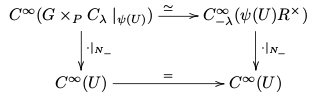
\includegraphics[scale=0.6]{master_master-6.png}
  \end{center}
  
  Here for $\lambda \in \mathbbm{C}$, and $V \subset \Xi$ invariant under
  multiplication by $\mathbbm{R}^{\times}$ we let $C^{\infty}_{- \lambda} ( V)
  \assign \left\{ f \in C^{\infty} ( V) | \forall \alpha \in
  \mathbbm{R}^{\times}, \; f ( \alpha \cdot) = | \alpha |^{- \lambda} f (
  \cdot) \right\}$. $G \times_P \mathbbm{C}_{\lambda} |_{\psi ( U)}$ denotes
  the portion of vector bundle $G \times_P \mathbbm{C}_{\lambda}$ above $\psi
  ( U)$. $\psi ( \cdot)$ denotes embedding of $N_- \simeq \mathfrak{n}_-
  \simeq \mathbbm{R}^{p, q}$ into $G / P$ (on the left) or into $\Xi$ (on
  right) The top map is a continuous $G$-equivariant isomorphism, defined for
  $f ( \cdot) \in C^{\infty} ( G \times_P \mathbbm{C}_{\lambda}) \simeq
  C^{\infty} ( G)_{\lambda}$ as $\tilde{f} \in C^{\infty}_{- \lambda} ( \Xi)$,
  $\tilde{f} ( g p_+) \assign f ( g)$ (here $p_+ \assign ( 1, 0_{p + q}, 1)
  \in \Xi$). The left vertical arrow is a restriction to an open subset $\psi
  ( U) P \subset G / P$. The right-vertical arrow is restriction to a
  submanifold $U \cdot ( 1, 0_{p + q}, 1) \subset \Xi$.
\end{lemma}

\begin{proof}
  We assume $U =\mathfrak{n}_-$ for simplicity, the proof for general $U$
  proceeds in precisely the same manner. First, we show that for smooth
  functions the top map is well-defined. Indeed, let $f \in C^{\infty} (
  G)_{\lambda} $ as in lemma \ref{sol:lem-unfold}. Then the map $\tilde{f} : g
  ( 1, 0_{p + q}, 1) \mapsto f ( g)$ on $G p_+$ is well-defined, as
  centralizer of $p_+$ equals to $M^0 N_+$ by proposition
  \ref{def-n-nots:prop-ximodel}, and for $\lambda : P \rightarrow
  \mathbbm{C}^{\times}$ is in lemma \ref{sol:lem-unfold}, we have $\lambda (
  M^0 N_+)$. Moreover, as action $G \curvearrowright \Xi$ is transitive by an
  argument similar to that of lemma \ref{doublePGP:lem-Gp-act-Xi}, we have $g
  p_+ \mapsto f ( g)$ being well-defined map $\tilde{f} \in C^{\infty} (
  \Xi)$.
  
  We next show that $\tilde{f}$ is also homogeneous of degree $- \lambda$, as
  we have for $\tilde{f} ( - g p_+) = \tilde{f} ( g m_0 p_+)$, for $m_0
  \assign \tmop{diag} ( - 1, 1_{p + q}, 1) \in M$ and hence $\tilde{f} ( g m_0
  p_+) \assign f ( g m_0) = f ( g_{}) = \tilde{f} ( g p_+)$, since $f \in
  C^{\infty} ( G)_{\lambda}$. Similarly, for $\alpha \in \mathbbm{R}_{> 0}$ we
  have $\tilde{f} ( \alpha g p_+) = \tilde{f} ( g a ( t) p_+)$ with $a ( t)$
  is in (\ref{def-n-nots:eq-A}) for $t = \ln ( \alpha)$, and hence the chain
  of equalities continues as $= \tilde{f} ( g a ( t) p_+) \assign f ( g a (
  t)) = e^{- \lambda t} f ( g) = \alpha^{- \lambda} f ( g p_+)$. This shows
  homogeneity.
  
  The fact that top map is isomorphic is implied by the fact that we can
  construct inverse map $C^{\infty}_{- \lambda} ( \Xi) \rightarrow C^{\infty}
  ( G)_{\lambda}$ by $\tilde{f} \mapsto f$, where we set $f ( g) \assign
  \tilde{f} ( g p_+)$. It can be similarly to above shown that this map is
  well-defined.
  
  Finally, the diagram commutes by direct inspection and proposition
  \ref{def-n-nots:prop-ximodel}.
\end{proof}

\begin{lemma}
  \label{sol:lem-holodep}Suppose $\Omega' \subset \Omega \subset
  \mathbbm{C}^m$ are an open set and $\kappa : \Omega \rightarrow \mathbbm{C}$
  is holomorphic. Suppose also that $U, V \subset \mathbbm{R}^k$ are open with
  $\psi : U \rightarrow V$ diffeomorphism, and $K_{\mu}^U \in \mathcal{D}' (
  U), K^V_{\mu} \in \mathcal{D}' ( V)$ are holomorphic in $\mu \in \Omega$.
  Then if for $f \in C^{\infty} ( U \rightarrow \mathbbm{R}_{> 0})$ we have
  $\forall \mu \in \Omega', \; f^{\kappa ( \mu)} K^U_{\mu} = \psi^{\ast}
  K^V_{\mu}$, then this also holds for every $\mu \in \Omega$.
\end{lemma}

\begin{proof}
  In the light of holomorphic rigidity, it suffices to show that $\psi^{\ast}
  K^V_{\mu}, f^{\kappa ( \mu)} K^U_{\mu} \in \mathcal{D}' ( U)$ are
  holomorphic in $\mu \in \Omega$. For $\psi^{\ast} K_{\mu}^V$ this is readily
  given by proposition \ref{holomorphicity-preserving:prop-pullback-holo}.
  Regarding $f^{\kappa ( \mu)} K^U_{\mu}$, lemma
  \ref{KR-normalization-recur:lem-mult-smth} implies that the latter can be
  seen as product of distributions and hence in the light of propositions
  \ref{holomorphicity-preserving:prop-tensor-holo} and
  \ref{holomorphicity-preserving:prop-pullback-holo}, it suffices to show that
  $f^{\kappa ( \mu)}$ is holomorphic when seen as an element of $\mathcal{D}'
  ( U)$. This can be proven directly.
\end{proof}

\subsection{Proofs}

\begin{definition}
  \label{sol:def-localaciton}For $\lambda \in \mathbbm{C}$ let $P'
  \curvearrowright G / P$ by left multiplication. Introduce also an embedding
  $\mathbbm{R}^{p, q} \ni w \mapsto \psi ( w) \assign n_- ( w) P \in G / P$.
  Suppose now that $( U, V)$ is a pair of open subsets of $\mathbbm{R}^{p, q}$
  and $p' \in P$ such that $\psi ( U) = p' \psi ( V)$. Then straightforward
  generalization of lemma \ref{KR-normalization-recur:lem-pull-comm-restr}
  tells us that the following diagram commutes
  \begin{center}
    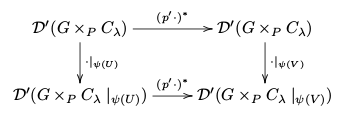
\includegraphics[scale=0.6]{master_master-7.png}
  \end{center}
  here $G \times_P \mathbbm{C}_{\lambda} |_{\psi ( U)}$ denotes portion of the
  bundle above $\psi ( U)$ and similarly for $\psi ( V)$. The top and bottom
  maps are isomorphisms. Now, pullback by $\psi ( \cdot)$ induces the
  isomorphism $\mathcal{D}' ( U) \rightarrow \mathcal{D}' ( V)$ so that the
  following map commutes:
  
  \begin{center}
    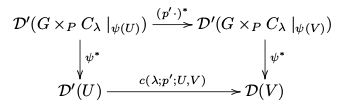
\includegraphics[scale=0.6]{master_master-8.png}
  \end{center}
  
  all maps of it are isomorphisms and we will call the one at the bottom by $c
  ( \lambda ; p' ; U, V) : \mathcal{D}' ( U) \rightarrow \mathcal{D}' ( V)$.
\end{definition}

\begin{definition}
  \label{sol:def-D'n}For $( \lambda, \nu) \in \mathbbm{C}^2$ we let
  $\mathcal{D}' ( \mathfrak{n}_-, \mathbbm{C}_{n - \lambda} \otimes
  \mathbbm{C}_{\nu})^{M' A', \mathfrak{n}'_+}$ to denote the space of $u \in
  \mathcal{D}' ( \mathbbm{R}^{p, q})$ such that for all $U, V, p'$ as in
  definition \ref{sol:def-localaciton} we have $u |_V = \nu^{} ( ( p')^{- 1})
  c ( n - \lambda ; p' ; U, V) u |_V$ with homomorphism $\nu : P' \rightarrow
  \mathbbm{C}^{\times}$ defined as in proposition
  \ref{def-n-nots:prop-degseries}.
\end{definition}

\begin{proof}
  (of prop. \ref{sol:prop-sol}) Proposition \ref{doublePGP:prop-pnp} implies
  that we can apply {\cite[thm. 3.16]{kobayashi2015symmetry}} and it
  immediately gives
  \[ \tmop{Hom}_{G'} ( I ( \lambda), J ( \nu)) \simeq \mathcal{D}' (
     \mathfrak{n}_-, \mathbbm{C}_{n - \lambda} \otimes \mathbbm{C}_{\nu})^{M'
     A', \mathfrak{n}'_+} \]
  Hence it suffices to show that $\mathcal{D}' ( \mathfrak{n}_-,
  \mathbbm{C}_{n - \lambda} \otimes \mathbbm{C}_{\nu})^{M' A',
  \mathfrak{n}'_+} =\mathcal{S} \tmop{ol} ( \mathbbm{R}^{p, q} ; \lambda,
  \nu)$ as in definition \ref{sol:def-sol}. Hence, we just need to concretely
  write down the $c ( \lambda ; p' ; U, V)$ map of \ref{sol:def-localaciton}.
  Moreover, as we have all arrows in commutative diagrams of definitions
  \ref{sol:def-localaciton} being continuous and mapping smooth to smooth,
  using approximation by smooth sections, we can assume that we have
  $\mathcal{D}'$ replaced by $C^{\infty}$ in all diagrams of definitions
  \ref{sol:def-localaciton}. Now, lemma \ref{sol:lem-commdiag} allows us to
  rewrite second commutative diagram of definition \ref{sol:def-localaciton}
  (with $\lambda$ replaced by $n - \lambda$, according to definition
  \ref{sol:def-D'n})
  
  \begin{center}
    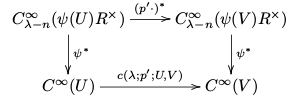
\includegraphics[scale=0.6]{master_master-9.png}
  \end{center}
  
  with an embedding $\psi : \mathbbm{R}^{p, q} \ni w \mapsto n_- ( w) \cdot (
  1, 0_{p + q}, 1) = ( 1 - Q ( w), 2 w, 1 + Q ( w)) \in \Xi$.
  
  Now, let $( p, U, V)$ be as in definition \ref{sol:def-localaciton}. If $p$
  is of the form
  \[ p \assign \left[ \begin{array}{ccc}
       1 & 0 & 0\\
       0 & m & 0\\
       0 & 0 & 1
     \end{array} \right] \in M' \]
  with $m \in O ( p, q)$ such that $m \cdot e_p = e_p$, then for $w \in
  \mathbbm{R}^{p, q}$ we have $p \cdot \psi ( w) = \psi ( m \cdot w)$.
  
  This implies that for $p, U, V$ as in definition \ref{sol:def-localaciton}
  with $p$ as above we should have $U = w V$ (and conversely all such triples
  satisfy definition \ref{sol:def-localaciton}) and $c ( p ; \lambda ; U, V) (
  F) ( \cdot) = F ( w \cdot)$.
  
  Next ,for an element $p \assign \tmop{diag} ( - 1, 1_{p + q}, - 1) \in M'$
  we have $p \cdot \psi ( w) = \psi ( - w)$. This implies that for $p, U, V$
  as in definition \ref{sol:def-localaciton} with $p$ as above we should have
  $U = - V$ (and conversely all such triples satisfy definition
  \ref{sol:def-localaciton}) and $c ( p ; \lambda ; U, V) ( F) ( \cdot) = F (
  ( - 1) \cdot)$.
  
  Next, for an element $a ( t) \in A'$ as in (\ref{def-n-nots:eq-A}), direct
  calculations show that we have we have $a ( t) \cdot \psi ( w) = e^t \psi (
  e^{- t} w)$ and hence for an element $f \in C^{\infty}_{\lambda - n}$ we
  would have $f ( a ( t) \psi ( w)) = e^{( \lambda - n) t} f ( \psi ( e^{- t}
  w))$, which implies that for $p, U, V$ as in definition
  \ref{sol:def-localaciton} with $p = a ( t)$ as above we should have $U =
  e^{- t} V$ (and conversely all such triples satisfy definition
  \ref{sol:def-localaciton}) and $c ( a ( t) ; \lambda ; U, V) ( F) ( \cdot) =
  e^{( \lambda - n) t} F ( e^{- t} \cdot)$.
  
  Finally, for $w \in \mathbbm{R}^{p, q}$ with $w_p = 0$ and an element $n_+ (
  w) \in N'_+$ as in (\ref{def-n-nots:eq-N+}), we observe that for $v \in
  \mathbbm{R}^{p, q}$ we have for $\psi_w ( \cdot)$ and $c_w ( \cdot)$ as in
  definition \ref{def-n-nots:def-n+invar}
  \[ n_+ ( w) n_- ( v) = c_w ( v) \cdot n_- ( \psi_w ( v)) \]
  whenever both sides make sense. Hence, for $p, U, V$ as in definition
  \ref{sol:def-localaciton} with $p = n_+ ( w)$ as above we should have $U =
  \psi_w ( V)$ (and conversely all such triples satisfy definition
  \ref{sol:def-localaciton}) and $c ( n_+ ( w) ; \lambda ; U, V) ( F) ( \cdot)
  = | c_w ( \cdot) |^{\lambda - n} F ( \psi_w ( \cdot))$.
  
  As the reasoning above tells us how $c ( \lambda ; p' ; U, V)$ are written
  for $p' \in M', A', N_+'$, we see that these are precisely equivalent to
  items of definition \ref{sol:def-sol} and thus Langlands decomposition of
  $P'$ tells us now that $\mathcal{D}' ( \mathfrak{n}_-, \mathbbm{C}_{n -
  \lambda} \otimes \mathbbm{C}_{\nu})^{M' A', \mathfrak{n}'_+} =\mathcal{S}
  \tmop{ol} ( \mathbbm{R}^{p, q} ; U, V)$.
\end{proof}

\begin{proof}
  (of prop. \ref{sol:prop-holocont}) In the light of the first item of remark
  after the definition \ref{sol:def-sol}, the conclusion is implied by lemma
  \ref{sol:lem-holodep}.
\end{proof}

\section{Non-equivalence of $N_+'$-invariance and
$\mathfrak{n}'_+$-invariance}\label{sec:n-nonequiv}

One might wonder whether it is possible to replace the item 4 of definition
\ref{sol:def-sol} with the differential of that (local) action of $N_+'$ on
$\mathbbm{R}^{p, q}$. We will call the latter $\mathfrak{n}_+'$-invariance.
Explicitly written, it becomes the system of differential equations
\begin{equation}
  \left[ (\lambda - n) \varepsilon_j x_j - \varepsilon_j x_j E + \frac{1}{2} Q
  (x) \frac{\partial}{\partial x_j} \right] F = 0, \hspace{1em} j = \{ 1, 2,
  \ldots, n \} \backslash \{ p \} \label{Ndiff}
\end{equation}
with $E \assign \sum_j x_j  \frac{\partial}{\partial x_j}$ and $\varepsilon_j
= + 1$ for $1 \leq j \leq p$ and $= - 1$ otherwise.

The purpose of this section is to show that this in general will not be
equivalent to the original definition. To this end we introduce

\begin{definition}
  \label{n-nonequiv:def-solprime}For $( \lambda, \nu) \in \mathbbm{C}^2$ and
  $U \subset \mathbbm{R}^{p, q}$ open, we let $\mathcal{S} \tmop{ol}'_{} ( U ;
  \lambda, \nu)$ to denote set of distributions $u \in \mathcal{D}' ( U)$,
  satisfying first three items of definition \ref{sol:def-sol} and equations
  (\ref{Ndiff}).
  
  We will also use the notation $\mathcal{S} \tmop{ol}_S' ( U ; \lambda, \nu)
  \assign \{ u \in \mathcal{S} \tmop{ol} ( U ; \lambda, \nu) | \tmop{supp} (
  u) \subset S \}$ for $S \subset U$ closed. We note that $\mathcal{S}
  \tmop{ol}'_S ( U ; \lambda, \nu) \supset \mathcal{S} \tmop{ol}_S ( U ;
  \lambda, \nu)$.
\end{definition}

\begin{proposition}
  $\mathcal{S} \tmop{ol}'_{} ( \mathbbm{R}^{p, q} ; \lambda, \nu)$ is strictly
  bigger than $\mathcal{S} \tmop{ol}_{} ( \mathbbm{R}^{p, q} ; \lambda, \nu)$
  for $\tmop{Re} (- \nu) > 0$ and $\tmop{Re} (\lambda + \nu - n) > 0$
\end{proposition}

\subsection{Auxiliary lemmas}

\begin{lemma}
  \label{lem67:lem-flip}For $p, q \in \mathbbm{Z}_{\geqslant 1}$ let $Q$:
  quadratic form on $\mathbbm{R}^{p, q}$. For $x, b \in \mathbbm{R}^{p, q}$ we
  let $c_b ( x) \assign 1 - 2 Q ( x, b) + Q ( x) Q ( b)$ and $\psi_b ( x)
  \assign ( x - Q ( x) b) / c_b ( x)$.
  
  We then have the following:
  \begin{enumerate}
    \item For $p \geqslant 1$ there exist $x^{( 0)}, b^{( 0)} \in
    \mathbbm{R}^{p, q}$ with $b^{( 0)}_p = 0$, such that $Q ( \psi_{b^{( 0)}}
    ( x^{( 0)})) > 0$ and $Q ( x^{( 0)}) < 0$;
    
    \item For $p \geqslant 2$ we can in addition make $\psi_{b^{( 0)}} ( x^{(
    0)})$ having it's $p$-th coordinate vanish.
  \end{enumerate}
\end{lemma}

\begin{proof}
  For the first item, it suffices to find $x^{( 0)}$ and $b^{( 0)}$ such that
  $Q ( x^{( 0)}) < 0$ and $Q ( x^{( 0)} - Q ( x^{( 0)}) b^{( 0)}) > 0$ (note
  that this will automatically grant $c_{b^{( 0)}} ( x^{( 0)}) \neq 0$, as $Q
  ( x - Q ( x) b) = Q ( x) ( 1 - 2 Q ( x, b) + Q ( x) Q ( b))$). Now, by
  assuming $x_i^{( 0)} = b^{( 0)}_i = 0$ for $i \neq p, p + 1$ (while still
  requiring $b_p^{( 0)} = 0$), and thus we have $Q ( x^{( 0)}) = ( x_p^{(
  0)})^2 - ( x_{p + 1}^{( 0)})^2$ and $Q ( x^{( 0)} - Q ( x^{( 0)}) b^{( 0)})
  = ( x_p^{( 0)})^2 - ( x_{p + 1}^{( 0)} - ( ( x_p^{( 0)})^2 - ( x_{p + 1}^{(
  0)})^2) b^{( 0)}_{p + 1})^2$. Hence, by taking arbitrary $x^{( 0)}$ with $Q
  ( x^{( 0)}) < 0$ and $b_{p + 1}^{( 0)} \assign x_{p + 1}^{( 0)} / ( ( x_p^{(
  0)})^2 - ( x_{p + 1}^{( 0)})^2)$, we get the required pair of elements of
  $\mathbbm{R}^{p, q}$. This shows the first item.
  
  Regarding the second item, we proceed similarly, except that this time we
  require $x_i^{( 0)} = 0$ for $i \neq p - 1, p + 1$, $b^{( 0)}_i = 0$ for $i
  \neq p$ and replace $x_p^{( 0)}$ by $x_{p - 1}^{( 0)}$ everywhere in
  computations of previous paragraph. As $\psi_{b^{( 0)}} ( x^{( 0)})$ and
  $x^{( 0)}$ have their $p$-th component being the same, this construction
  suffices.
\end{proof}

\subsection{Proofs}

\begin{proof}
  Having fixed $(\lambda, \nu) \in \C^2$ such that $\tmop{Re} (- \nu) > 0$ and
  $\tmop{Re} (\lambda + \nu - n) > 0$ consider the distribution
  \[ K_+ (x) \assign | x_p |^{\lambda + \nu - n} Q_+^{- \nu} (x) . \]
  It is directly verified that it belongs to $\mathcal{S} \tmop{ol}' (
  \mathbbm{R}^{p, q} ; \lambda, \nu)$. Suppose now that $K_+ \in \mathcal{S}
  \tmop{ol} ( \mathbbm{R}^{p, q} ; \lambda, \nu)$. As we have $K_+$ vanishing
  outside $\{ Q \geqslant 0 \} \subset \mathbbm{R}^{p, q}$, $N_+'$-invariance
  and lemma \ref{lem67:lem-flip} imply that $K_+$ vanishes at some open subset
  of $\{ Q > 0 \}$. But this clearly contradicts the way we defined $K_+$.
\end{proof}

\begin{thebibliography}{CK{\O}P11}
  \bibitem[CK{\O}P11]{clerc2011generalized}J.-L. Clerc, T.~Kobayashi,
  B.~{\O}rsted, and M.~Pevzner. {\newblock}Generalized bernstein--reznikov
  integrals. {\newblock}\tmtextit{Mathematische Annalen}, 349(2):395--431,
  2011.
  
  \bibitem[CP82]{chazarain2011introduction}J.~Chazarain and A.~Piriou.
  {\newblock}\tmtextit{Introduction to the theory of linear partial
  differential equations}. {\newblock}North-Holland Publishing Company, 1982.
  
  \bibitem[Del98]{delorme1998plancherel}P.~Delorme. {\newblock}Plancherel
  formula for reductive symmetric spaces. {\newblock}147(2):417--452, 1998.
  
  \bibitem[Far79]{faraut1979distributions}J.~Faraut. {\newblock}Distributions
  sph{\'e}riques sur les espaces hyperboliques. {\newblock}\tmtextit{J. Math.
  Pures Appl.}, 58:369--444, 1979.
  
  \bibitem[GGP12]{gan2011symplectic}W.~T. Gan, B.~H. Gross, and D.~Prasad.
  {\newblock}Sur les conjectures de Gross et Prasad.
  {\newblock}\tmtextit{Ast{\'e}risque}, 2012.
  
  \bibitem[GGV66]{gelfand1966generalized}I.~M. Gelfand, M.~I. Graev, and N.~Y.
  Vilenkin. {\newblock}\tmtextit{Generalized functions. Vol. 5, Integral
  geometry and representation theory}. {\newblock}Academic Press, 1966.
  
  \bibitem[GS69]{gelfand1980distribution}I.~M. Gelfand and G.~E. Shilov.
  {\newblock}\tmtextit{Generalized functions. Vol. 1, Properties and
  operations}. {\newblock}Academic Press, 1969.
  
  \bibitem[HC76]{harishchandra1978harmonic}Harish-Chandra. {\newblock}Harmonic
  analysis on real reductive groups III. The Maass-Selberg relations and the
  Plancherel formula. {\newblock}\tmtextit{Annals of Mathematics},
  104(1):117--201, 1976.
  
  \bibitem[H{\"o}r83]{hormander1983analysis}L.~H{\"o}rmander.
  {\newblock}\tmtextit{The Analysis of Linear Partial Differential Operators:
  Vol.: 1.: Distribution Theory and Fourier Analysis}.
  {\newblock}Springer-Verlag, 1983.
  
  \bibitem[HT93]{howe1993homogeneous}R.~E. Howe and E.-C. Tan.
  {\newblock}Homogeneous functions on light cones: the infinitesimal structure
  of some degenerate principal series representations.
  {\newblock}\tmtextit{Bulletin of the American Mathematical Society},
  28(1):1--74, 1993.
  
  \bibitem[Juh09]{juhl2009families}A.~Juhl. {\newblock}\tmtextit{Families of
  conformally covariant differential operators, Q-curvature and holography},
  volume 275. {\newblock}Springer Science \& Business Media, 2009.
  
  \bibitem[KM14]{kobayashi2014classification}T.~Kobayashi and T.~Matsuki.
  {\newblock}Classification of finite-multiplicity symmetric pairs.
  {\newblock}\tmtextit{Transformation Groups}, 19(2):457--493, 2014.
  
  \bibitem[K{\O}03]{KO1}T.~Kobayashi and B.~{\O}rsted. {\newblock}Analysis on
  the minimal representation of \tmtextrm{O}$(p, q)$.\tmtextrm{I}. Realization
  via conformal geometry. {\newblock}\tmtextit{Adv. Math.}, 180:486--512,
  2003.
  
  \bibitem[Kob94]{kobayashi1994discrete1}T.~Kobayashi. {\newblock}Discrete
  decomposability of the restriction of $A_q (\lambda)$ with respect to
  reductive subgroups and its applications. {\newblock}\tmtextit{Inventiones
  mathematicae}, 117(1):181--205, 1994.
  
  \bibitem[Kob98a]{kobayashi1998discrete2}T.~Kobayashi. {\newblock}Discrete
  decomposability of the restriction of $A_q (\lambda)$ with respect to
  reductive subgroups II: Micro-local analysis and asymptotic K-support.
  {\newblock}\tmtextit{Annals of mathematics}, pages 709--729, 1998.
  
  \bibitem[Kob98b]{kobayashi1998discrete3}T.~Kobayashi. {\newblock}Discrete
  decomposability of the restriction of $A_q (\lambda)$ with respect to
  reductive subgroups III. restriction of Harish-Chandra modules and
  associated varieties. {\newblock}\tmtextit{Inventiones mathematicae},
  131(2):229--256, 1998.
  
  \bibitem[Kob15]{kobayashi2015program}T.~Kobayashi. {\newblock}A program for
  branching problems in the representation theory of real reductive groups.
  {\newblock}In \tmtextit{Representations of Reductive Groups}, pages
  277--322. Springer, 2015.
  
  \bibitem[KP15a]{kobayashi2015differential1}Toshiyuki Kobayashi and Michael
  Pevzner. {\newblock}Differential symmetry breaking operators: I. General
  theory and F-method. {\newblock}\tmtextit{Selecta Mathematica}, pages 1--45,
  2015.
  
  \bibitem[KP15b]{kobayashi2015differential2}Toshiyuki Kobayashi and Michael
  Pevzner. {\newblock}Differential symmetry breaking operators: II.
  Rankin--Cohen operators for symmetric pairs. {\newblock}\tmtextit{Selecta
  Mathematica}, pages 1--65, 2015.
  
  \bibitem[Kra82]{krantz1982function}S.~G. Krantz.
  {\newblock}\tmtextit{Function theory of several complex variables}.
  {\newblock}Pure and applied mathematics. Wiley, 1982.
  
  \bibitem[KS15]{kobayashi2015symmetry}T.~Kobayashi and B.~Speh.
  {\newblock}Symmetry breaking for representations of rank one orthogonal
  groups. {\newblock}\tmtextit{Memoirs of the American Mathematical Society},
  238(1126), 2015.
  
  \bibitem[OM84]{oshima1984description}T.~Oshima and T.~Matsuki. {\newblock}A
  description of discrete series for semisimple symmetric spaces.
  {\newblock}\tmtextit{Adv. Stud. Pure Math}, 4:331--390, 1984.
  
  \bibitem[Wal88]{wallach1988real}N.~Wallach. {\newblock}\tmtextit{Real
  Reductive Groups I}, volume 132 of \tmtextit{Pure and Applied Mathematics}.
  {\newblock}Academic press, 1988.
  
  \bibitem[War71]{warner1971foundations}F~Warner. {\newblock}Foundations of
  differential geometry and Lie groups. {\newblock}\tmtextit{Scott Foresman
  and Company, Glenview}, 1971.
\end{thebibliography}

\end{document}
